\documentclass[12pt,oneside]{report}
\usepackage[a4paper,width=150mm,top=25mm,bottom=25mm]{geometry}
\usepackage{amsmath,amsthm,amssymb}
\usepackage[utf8]{vietnam}
\usepackage{pdfpages}   %Cover page with pdf
\usepackage{listings}
\usepackage[numbers]{natbib}
\usepackage{enumitem}
\usepackage{graphicx}
\usepackage{subcaption}
\usepackage[nottoc]{tocbibind}
\usepackage{url}
\usepackage{hyperref}
\usepackage{algorithm}
\usepackage{algpseudocode}
\usepackage{pifont}
\usepackage{subcaption} %subfigure
\usepackage{cases} 
\usepackage{scrextend}
\usepackage{marginnote}
\addtokomafont{labelinglabel}{\sffamily}
\usepackage{fancyhdr} %Header
\pagestyle{fancy}
\fancyhead[RO,LE]{}
\usepackage{afterpage}

\newcommand\blankpage{%
    \null
    \thispagestyle{empty}%
    \newpage}
    
\raggedbottom




%--------------Define list of some thing ---------%
\usepackage{tocloft} %define some thing your own
\newcommand{\listexamplename}{Bảng tham chiếu từ chuyên nghành}
\newlistof{word}{wor}{\listexamplename}
\newcommand{\word}[2]{%Số 2 ở đây biểu thị cho số biến truyền vào
    \refstepcounter{word}%
    \textit{#1 (#2)}%
    \addcontentsline{wor}{word}
    {\protect
    \begin{tabular}{p{7.2cm}p{5.9cm}}
        #1 & #2\\
    \end{tabular}
    }
}


\DeclareMathOperator*{\argmaxA}{arg\,max} % Jan Hlavacek
\usepackage{lipsum} %split subfigure

\captionsetup{compatibility=false}
\renewcommand{\baselinestretch}{1.5}
\begin{document}

\begin{titlepage} 
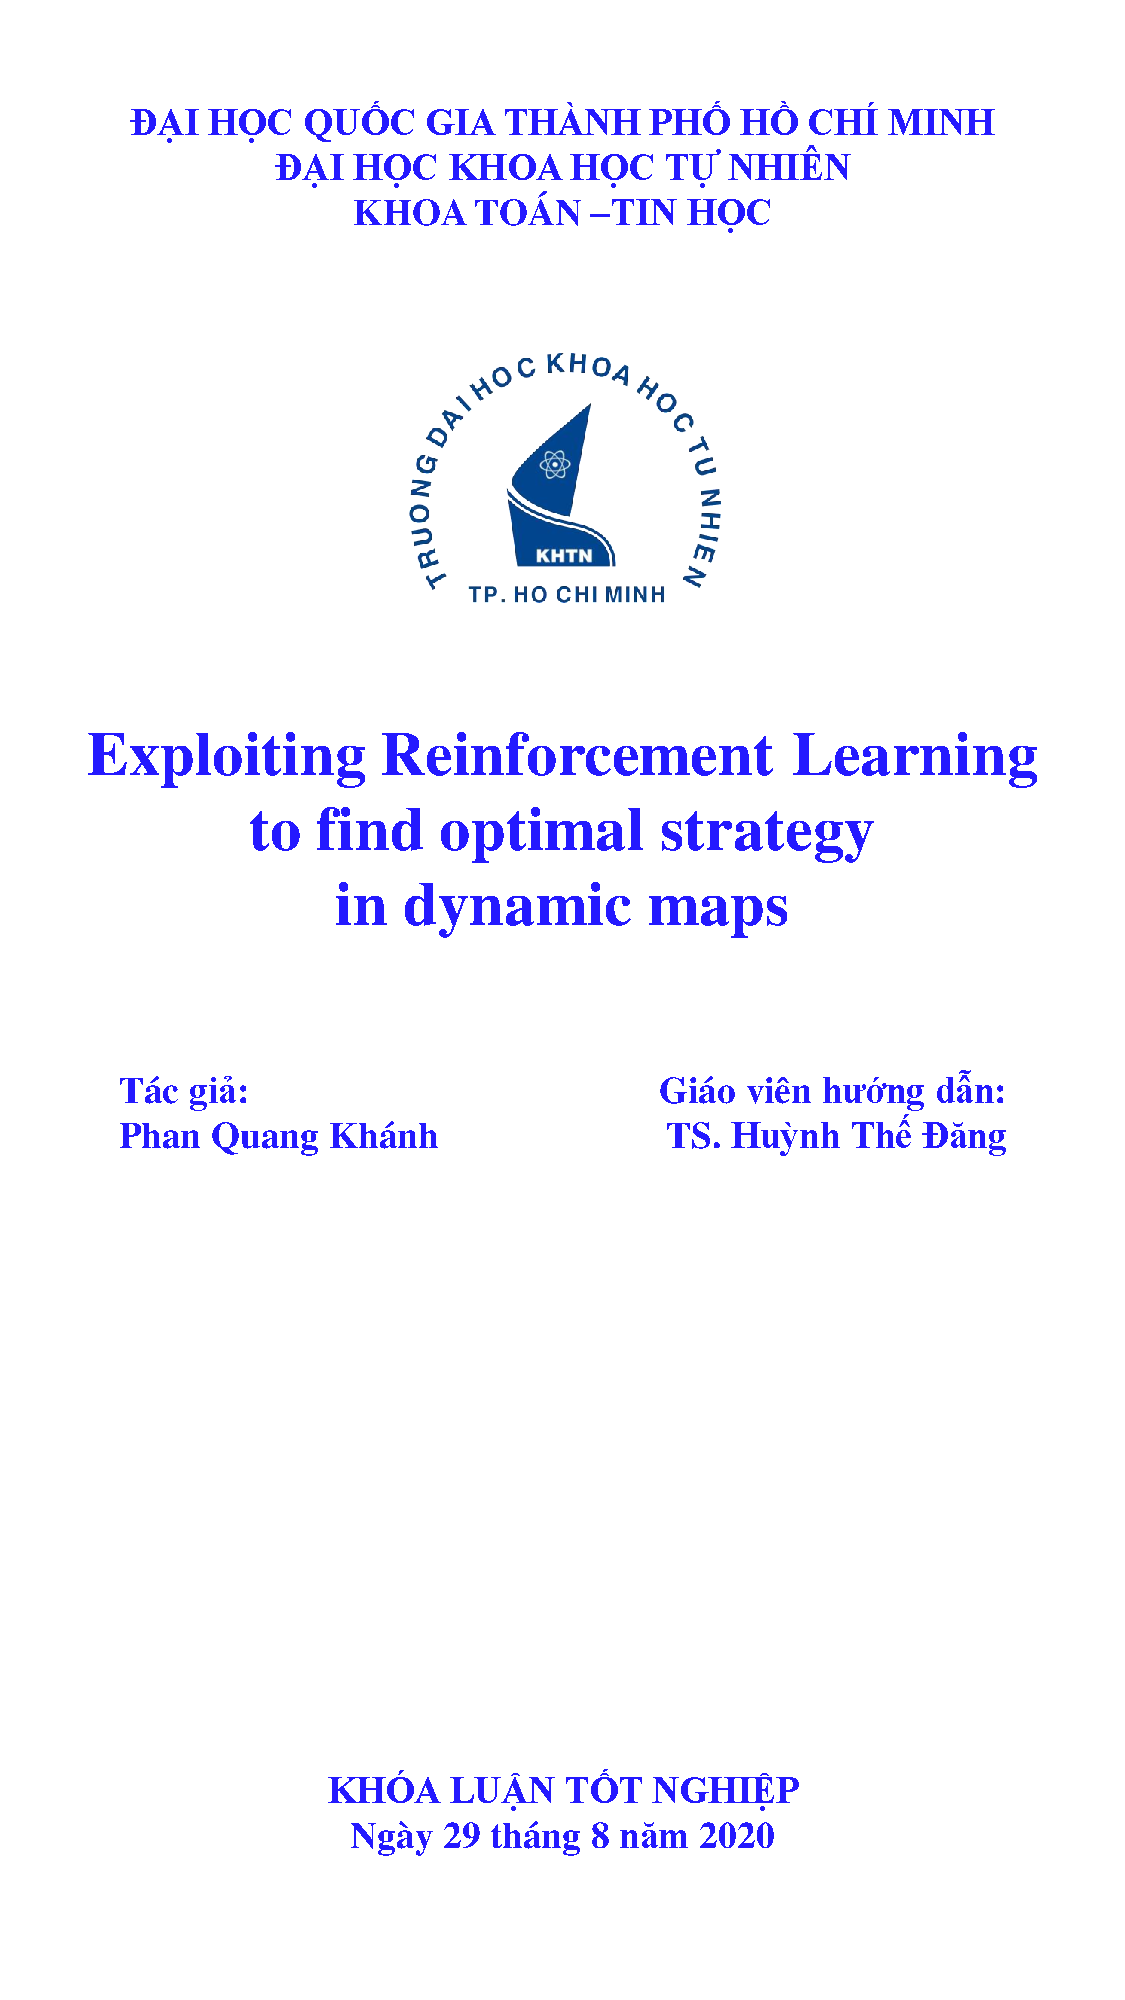
\includepdf{Pic/cover.pdf}
\end{titlepage}
\clearpage
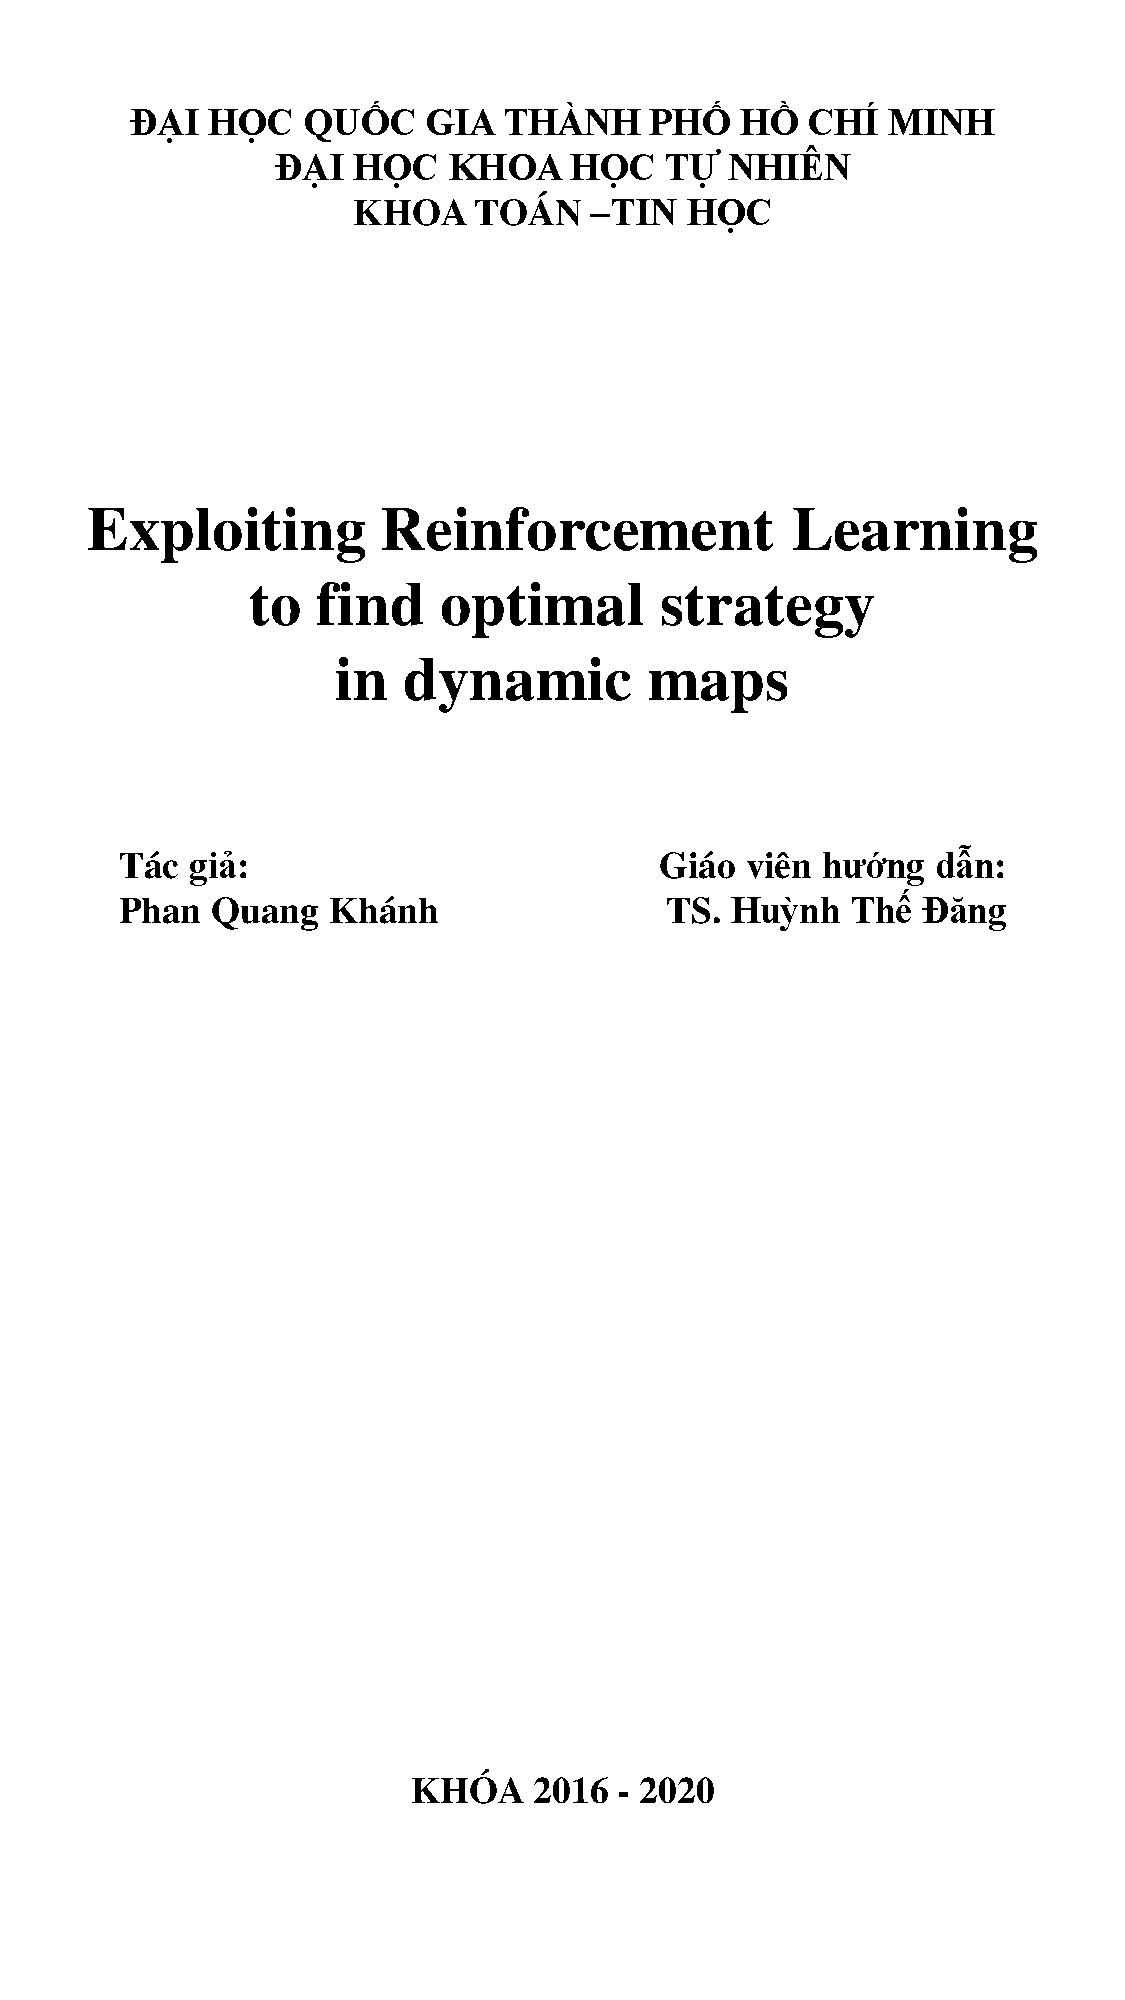
\includepdf[page=-]{Pic/cover_BACKUP.pdf}
\clearpage
%---------------------------------------------------------------------------------
\chapter*{Lời cảm ơn}
Trong quá trình thực hiện khóa luận, tôi gặp rất nhiều khó khăn từ ý tưởng đến việc thực hiện. Để vượt qua các khó khăn không chỉ nhờ sự nỗ lực tìm hiểu và học tập của bản thân, mà còn có sự giúp đỡ rất lớn từ quý Thầy Cô, bạn bè và gia đình:
\begin{itemize}
\item Đầu tiên, tôi rất biết ơn về tận tình từ Thầy hướng dẫn của tôi, Tiến sĩ Huỳnh Thế Đăng. Với nhiều kinh nghiệm trong lĩnh vực máy học, cũng như giảng dạy, Thầy đã mang đến cho tôi nhiều ý tưởng cũng như động lực trong việc thực hiện khóa luận. Tôi thực sự biết ơn khi là một sinh viên của Thầy.
\item Tiếp theo, khóa luận này không thể thực hiện được khi không có sự hỗ trợ tích cực từ các Thầy cô trong phòng Bộ môn Ứng dụng Tin học khi cung cấp một môi trường học tập với đầy đủ các công cụ cần thiết cho khóa luận.
\item Cuối cùng, tôi muốn gửi lời cảm ơn đến quý Thầy Cô trong khoa Toán-Tin học, trường Đại học Khoa học Tự nhiên đã tận tình dạy dỗ trong suốt bốn (04) năm học đã truyền đạt những kiến thức hữu ích nhất giúp tôi tích lũy nền tảng cơ bản.
\end{itemize}
Trong quá trình thực hiện và hoàn thành khóa luận này, mặc dù có sự cố gắng tối đa nhưng có thể không tránh khỏi sai sót. Vì thế kính mong nhận được sự đóng góp ý kiến từ quý Thầy Cô và các bạn để hoàn thiện hơn.

\begin{flushright}
{\it Tp.HCM, ngày 29 tháng 08 năm 2020}

Người thực hiện\hskip 2cm\quad

{\bf PHAN QUANG KHÁNH} \hskip 0.5cm \quad\
 \end{flushright}
\clearpage
\tableofcontents
\clearpage
\listoffigures 
\clearpage
\phantomsection
\listofword\label{listofword}
\addcontentsline{toc}{chapter}{Bảng tham chiếu từ chuyên ngành}
\clearpage
\chapter{Giới thiệu}
\section{Đặt vấn đề}
Sau sự thành công của DeepMind năm 2013 với bộ máy chơi game đình đám một thời Atari\cite{DBLP:journals/corr/MnihKSGAWR13}, \word{Học Tăng cường}{Reinforcement Learning}đã bước vào các ngành công nghiệp trò chơi điện tử nhằm đạt giải quyết được những bài toán phức tạp và tạo nên những thử thách mới cho con người. Đây là bước ngoặt quan trọng cho sự trở lại mãnh liệt sau khoảng thời gian lặng tiếng của phương pháp học tăng cường khi AlphaGo\cite{44806} đánh bại kỳ thủ xuất xắc nhất lúc bấy giờ trong bộ môn cờ vây năm 2017. Tiếp sau đó là sự thành công của OpenAI trong trò chơi Dota2\cite{openai2019dota} , những người chơi được đánh giá mạnh nhất của trò chơi vào thời điểm này "ngả mũ" trước những nhân vật được máy điều khiển . Với bảng thành tích như vậy, học tăng cường thực sự giải quyết được những vấn đề mà con người khó có thể đạt được tuy nhiên việc áp dụng học tăng cường vào thực tế rất khó khăn theo như\cite{DBLP:journals/corr/abs-1904-12901}.\\
\\
The World’s Hardest Game\cite{WHGwebsite} (WHG) là một trò chơi trực tuyến nổi tiếng trong năm 2015 với vòng chơi khó nhưng đủ khiến kích thích người chơi cố gắng vượt qua bởi tưởng “dễ nhưng không dễ” của nó. Trong trò chơi, người chơi có thể di chuyển bằng 5 hướng (trên, dưới, trái, phải, đứng yên) với mục đích hoàn thành cách thức chơi của mỗi vòng. Để hoàn thành một vòng chơi, người chơi phải thu thập hết các đồng xu, tránh va phải các vật cản và di chuyển đến vùng qua màn. Vì các yếu tố của trò chơi thảo mãn \cite{MarkovProperty} và độ khó của trò chơi nên WHG là ứng cử viên tốt cho học tăng cường.\\
\begin{figure}[h]
    \centering
    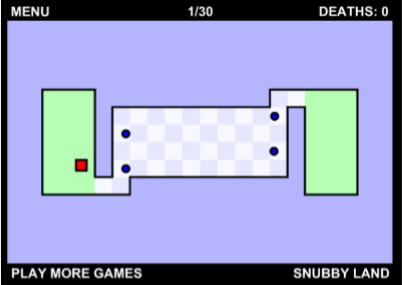
\includegraphics[height=0.3\textheight]{Pic/lv1game.png}
    \caption[Vòng đầu tiên của WHG]{\textit{Hình ảnh vòng đầu tiên của WHG}, trò chơi chia làm 3 phần: phần xanh lá cây trái cùng là vùng an toàn, phần xanh phải cùng là vùng đích chiến thắng và còn lại là vùng hoạt động của các vật cản. Trên hình, biểu tượng ô vuông màu đỏ biểu thị cho robot và biểu tượng tròn màu xanh biểu thị cho các vật cản chuyển động.}
    \label{fig:lv1game}
\end{figure}
\section{Mục tiêu}
Một vài các tiếp cận của học tăng cường vào WHG như sử dụng \word{Giải thuật Di truyền}{Genetic Algorithm}của \cite{WHG_codebullet} hay đưa ra các trò chơi nhỏ của \cite{WHG_yasyf}, cả hai cách tiếp cận trên đều không đưa ra được lời giải cho WHG nhưng đã để lại nhiều kinh nghiệm cho nhóm tác giả trong việc chinh phục WHG.\\
Mục tiêu chính của khóa luận này là thực hiện huấn luyện một \word{robot}{agent}\footnote{Nghĩa của agent ở đây nhóm tác giả chọn đại diện cho sự vật này là robot để thể hiện cho sự vật cần học các tri giác vì "tác tử" được dùng để gọi agent có thể khiến người đọc nhầm lẫn.} đủ thông minh để chinh phục WHG và đường đi tìm được phải tối ưu. Ngoài ra sau các thử nghiệm của \cite{WHG_yasyf} khi sử dụng \word{Học Tăng cường Chuyên sâu}{Deep Q-learning}vào WHG nhưng chưa kết quả không khả quan, vì vậy chúng tôi sẽ đưa ra các giải pháp để áp dụng học tăng cường vào WHG cùng với các tùy chỉnh sẽ đưa ra trong xuyên suốt khóa luận.\\
Kết quả và thực nghiệm sau cùng của nhóm sẽ được cập nhật tại:\\
\textbf{\href{https://github.com/pqkhanh561/thesis}{https://github.com/pqkhanh561/thesis}}

\section{Cấu trúc khóa luận}
Theo sau chương giới thiệu này, khóa luận sẽ bao quát lý thuyết học tăng cường và các thực nghiệm trên các môi trường đề xuất.
\begin{labeling}{alligator}
\item [\textbf{Chương 1:}] Phần giới thiệu đưa ra tổng quan về khóa luận, bao gồm các tiếp cận tới bài toán hiện tại, động lực để nhóm thực hiện và cuối cùng là mục tiêu của của nhóm tác giả hướng đến.
\item [\textbf{Chương 2:}] Đưa ra lý thuyết cơ bản của học tăng cường và sự hình thành Q-learning.
\item [\textbf{Chương 3:}] Bao quát các bước thực hiện khóa luận, bao gồm các cài đặt để có thể thực hiện huấn luyện và đưa ra một số giả thiết cùng các giải pháp cải thiện.
\item [\textbf{Chương 4:}] Trình bày các kết quả huấn luyện của các mô hình được đề xuất, thảo luận các bước đi tiếp theo sau những thay đổi trong quá trình.
\item [\textbf{Chương 5:}] Kết luận từ các kết quả của nhóm.
\item [\textbf{Chương 6:}] Nhóm tác giả đưa ra các hướng đi trong tương lai cho đề tài.
\end{labeling}


\chapter{Phương pháp Học Tăng cường}
\section{Vấn đề của học tăng cường}
Học tăng cường được miêu tả trong \cite{RLSuttonBook}, là tổng hợp các thuật toán giúp cho robot học được qua môi trường bằng phương pháp thử. Khác với những thuật toán máy học khác, robot không được biết trước hành động chính xác tiếp theo để thực hiện. Thay vào đó, robot phải tự khám phá môi trường và tối ưu hóa lượng phần thưởng tương lai có thể nhận, thường mục tiêu là tìm kiếm điểm đích và được thưởng một lượng lớn sau cùng.
\subsection{Môi trường}
\word{Môi trường}{Environment}được cấu tạo từ thế giới cho robot tương tác và học. Trong thực tế, môi trường có thể là điều khiển cánh tay robot, thăng bằng một thanh gậy, hình ảnh 2D và 3D trích xuất từ camera. Nó có thể bao gồm toàn bộ thế giới ảo, những bài đăng (twitter/ facebook) hay là máy chơi ảo (Atari, OpenAI Gym). Những môi trường từ đơn giản đến phức tạp xung quanh cuộc sống ta đều có thể là ứng cử viên cho robot để học. Để xác định một cách rõ ràng toàn bộ môi trường là điều rất khó, trong bài khóa luận này nhóm tác giả sẽ dùng một vector để thể hiện
 \word{Trạng thái}{State}của môi trường. Một trạng thái trong môi trường được biểu diễn bởi không gian $N$ chiều chứa trạng thái của một môi trường $D$.
\begin{align*}
    s_t \in D,\quad\quad\quad s_t \in \mathbb{R}^N
\end{align*}
Trong đó $s_t$ là một trạng thái cụ thể tại thời điểm $t$ và $D$ bao gồm tất cả các trạng thái mà robot có thể gặp. Số chiều $N$ của $\mathbb{N}$ phụ thuộc vào vấn đề đang giải quyết. Một trạng thái phù hợp sẽ ảnh hưởng đến trực tiếp đến quá trình học của robot. Với mỗi vấn đề, có rất nhiều cách để biểu diễn trạng thái, việc xác định trạng thái có đặc trưng tốt sẽ giúp cho việc học của robot khả thi và tiết kiệm thời gian.
\subsection{Phần thưởng/Đích}
\word{Phần thưởng}{Reward}đóng vài trò chủ chốt trong việc quyết định học như thế nào của robot. Ví dụ với phần thưởng dương sẽ thúc đẩy robot làm việc đó nhiều hơn. Ngược lại, robot sẽ không thích làm những việc mà nó bị phạt bởi phần thưởng âm. Theo nghiên cứu của \cite{RLSuttonBook}, tối ưu tổng của các phần thưởng trong tương lai là mục tiêu của robot:\\
\begin{equation}\label{returnbegin}
    R_t = r_{t+1} + r_{t+2} + \dots +r_T\\
\end{equation}
Trong đó $R_t$ là tổng tích lũy các phần thưởng từ thời điểm cụ thể $t$ đến $T$ với $ T$ thường là thời điểm robot hết được tương tác với môi trường nữa. Tổng quát, trong những môi trường rời rạc, có thể viết lại công thức \ref{returnbegin} như sau:
\begin{equation}\label{returnStochastic}
    R_t = \sum^T_{k=0}r_{t+k+1}
\end{equation}
Tuy nhiên, không phải lúc nào các phần thưởng mà robot có thể nhận được trong tương lai với một trạng thái cụ thể là như nhau. Trong \cite{RLSuttonBook}, tham số $\gamma$ được biết là \word{Hệ số Chiết khấu}{Discount Factor} với vai trò khiến robot cân nhắc trước khi chọn một hành động bất kỳ. Ví dụ nếu $\gamma$ tiến gần đến không, robot sẽ xem xét các hành động gần trạng thái hiện tại nào giá trị nhất. Ngược lại, robot sẽ hoạt động một cách tham lam chọn những hành động mang lượng phần thưởng lớn. 
%xem lại định nghĩa gamma
\begin{equation}\label{finalReturn}
    R_T = \sum^T_{k=0}\gamma^kr_{t+k+1}
\end{equation}
\section{Quá trình Quyết định Markov}\label{MDP}
Để thực hiện việc ra quyết định, một hệ thống tổng hợp nhiều luật lệ có thể mô hình hóa thực tế dưới dạng toán học là điều cần thiết. Để đơn giản hóa, tính chất "không nhớ" trong thống kê được sử dụng bằng \textit{tính chất Markov}\cite{MarkovProperty}. Mở rộng của  \textit{chuỗi Markov}, việc thêm vào các hành động để cho ra những kết quả đầu ra khả thi và phần thưởng được xem là nhân tố giúp cho robot phân biệt được những trạng thái có giá trị quan trọng, chúng tôi nhắc lại định nghĩa của 
\word{Quá trình Quyết định Markov}{Markov Decision Processes}(MDP)\cite{AIbook}. Xuyên suốt khóa luận, các môi trường được sử dụng sẽ xây dựng  dựa trên MDP.\\
Một cấu trúc chuẩn của học tăng cường theo MDP, sẽ bao gồm:
\begin{itemize}
    \item \textbf{Một tập hợp hữu hạn trạng thái $D$}, sẽ bao gồm tất cả những biểu diễn của môi trường.
    \item \textbf{Một tập hợp hữu hạn các hành động}, bao gồm tất cả hành động của robot tại một thời điểm bất kỳ.
    \item \textbf{Một hàm phần thưởng} $r = \psi(s_t, a_t, s_{t+1})$, được xác định là phần thưởng khi robot thực hiện hành động $a_t$ từ trạng thái $s_t$, kết quả là $s_{t+1}$.
    \item \textbf{Một mô hình chuyển tiếp} $T(s_t,a_t,s_{t+1}) = p(s_{t+1}|s_t,a_t)$, là xác xuất xảy ra trạng thái $s_{t+1}$ khi thực hiện hành động $a_t$ tại trạng thái $s_t$.
\end{itemize}
\section{Các hàm cải thiện hành vi}
Về mặt toán học, hành vi của robot chưa được định nghĩa. Nhưng chúng ta luôn mong muốn robot sẽ dần dần đạt được nhiều phần thưởng qua mỗi \word{tập}{episode}, cách phản ứng này được xem là cách học tăng cường tức cứ thử nhiều lần cho đến khi học được. Vậy hành vi của robot trở thành một tiền đề đơn giản: "Hành động nào cần thực hiện tại mỗi trạng thái?"
\subsection{Chính sách}
Mỗi hành vi của robot được quyết định bởi \word{Chính sách}{Policy}, được định nghĩa là một ánh xạ xác định hành động thực hiện tại mỗi trạng thái. Một chính sách có thể xác định khi chắc chắn hành động được thực hiện với một trạng thái xác định, và có thể ngẫu nhiên khi hành động tại trạng thái có khả năng xảy ra. Do đó, một chính sách xác định có thể được biểu diễn như sau:
\begin{equation}\label{deterpolicy}
    \pi(s_t)=a_t\quad,\quad\quad s_t\subset D\quad a_t\subset A
\end{equation}
Nếu hành động là ngẫu nhiên thì chính sách có thể chuyển thành một phân phối xác suất của $a_t$ tại $s_t$ thì có thể biểu diễn như sau:
\begin{equation}\label{stochastic_policy}
\pi(a_t|s_t) = p_i\quad,\quad\quad s_t \subset D\quad a_t\subset A \quad 0\le p_i \le 1
\end{equation}
Về mặt lý thuyết, chính sách có được nhiều lượng phần thưởng nhất được xem là chính sách tối ưu, ký hiệu là $\pi^*$. Để đạt đến mức tối ưu cần áp dụng thuật toán kết hợp với một chiến thuật \word{Khám phá}{Exploration}cho đến khi hội tụ và một lượng đủ số tập cần học. 
\subsection{Hàm Giá trị}
Một \word{Hàm Giá trị}{Value Function} sẽ đánh giá độ hữu dụng của chính sách khi biết trước trạng thái. Theo \ref{finalReturn}:
\begin{equation}\label{Value_function}
    V:V^\pi \longleftarrow \mathbb{R}, \quad V^\pi(s)=\mathbb{E}_\pi\left[R_t|s_t=s\right]=\mathbb{E}_\pi\left[\sum^\infty_{i=0}\gamma^ir_{t+i+1}\Big|s_t=s\right]
\end{equation}
Hơn thế nữa, hàm giá trị có thể được ước lượng bằng phương pháp "thử", bởi vì giá trị kỳ vọng sẽ thu được từ kinh nghiệm của robot. Nhờ vào tính chất của quy hoạch động nên việc khai triển hàm giá trị hiển nhiên vì có thể tính hàm bằng phương pháp đệ quy. Theo \ref{Value_function}:
\begin{align}
    \nonumber
    V^\pi(s) = \mathbb{E}_\pi[R_t|s_t=s] &= \mathbb{E}_\pi\left[\sum^{\infty}_{i=0}\gamma^ir_{t+i+1}\Big|s_t=s\right]\\
    &=\mathbb{E}_\pi\left[r_{t+1}+\gamma\sum^{\infty}_{i=0}\gamma^i + r_{t+i+2}\Big|s_t=s\right]\label{unfoldValueFunction}
\end{align}
Nếu chính sách chúng ta đang xét là ngẫu nhiên thì biểu thức \ref{unfoldValueFunction} có thể được khai triển thành \textit{biểu thức Bellman} của $V^\pi$\cite{RLSuttonBook}:
\begin{equation}
    V^\pi(s) = \sum_a\pi(a|s)|\sum_{s_{t+1}}p(s_{t+1}|s_t,a)\left[r(s,a,s_{t+1}) + \gamma V^\pi(s_{t+1})\right]
\end{equation}
\subsection{Hàm chất lượng}
Có rất nhiều phương pháp có thể thu được chính sách "gần tối ưu", một trong những phương pháp đó là sử dụng một \word{Hàm Chất lượng}{Quality Function}\cite{RLSuttonBook} để đánh giá chất lượng của việc chọn một hành động để thực hiện tại một trạng thái xác định, sẽ được đề cập trong phần \ref{Qlearning}. Hàm chất lượng có định nghĩa tương tự như hàm giá trị khi biết trước hành động được thực thi. Nó bao gồm phần thưởng trong một khoảng thời gian dài khi áp dụng một hành động tại một trạng thái với chính sách xác định\cite{RLSuttonBook}:
\begin{align}
    \nonumber
    Q:S\times A \longrightarrow \mathbb{R}\quad Q^\pi(s,a)&=\mathbb{E}_\pi[R_t|s_t=s, a_t=a]\\
    &=\mathbb{E}_\pi\left[\sum^\infty_{i=0}\gamma^ir_{t+i+1}\Big| s_t=s, a_t=a\right]
\end{align}

Nếu một chính sách tối ưu $\pi^*$ đã được xác định thì giá trị của một trạng thái $V^{\pi^*}(s_t)$ bằng với hàm chất lượng $Q^{\pi^*}(s_t,a_t)$ khi thực một hành động tối ưu\cite{RLSuttonBook}:
\begin{equation}\label{Q-function}
    s_t\subset D \quad a_t \subset A \quad V^{\pi^*} (s_t)=Q^{\pi^*}(s_t,a_t) = \argmaxA_aQ^{\pi^*}(s_t,a_t)
\end{equation}
\vspace{1cm}
\section{Q-learning}\label{Qlearning}
Một trong những đột phá trong học tăng cường là sự phát triển của thuật toán \word{Thuật toán kiểm soát sự khác biệt theo thời gian không chính sách}{off-policy TD control algorithm} được biết là \textit{Q-learning} (Watkins, 1989). Sở dĩ Q-learning được xem là thuật toán không chính sách là vì việc ước lượng hàm chất lượng tối ưu độc lập với chính sách hiện thời. Thuật toán chọn một chính sách khác để có thể cập nhật hàm chất lượng tương tự ban đầu.
\begin{equation}
    Q:S\times A \longrightarrow \mathbb{R}
\end{equation}
\begin{equation}\label{Q-learning update}
    Q(s_t,a_t)\leftarrow Q(s_t,a_t) + \alpha(r_{t+1} + \gamma \max_aQ(s_{t+1},a_{t+1})-Q(s_t,a_t))
\end{equation}
Tham số $\alpha$ trong phương trình \ref{Q-learning update} là \word{Tỷ số học}{Learning rate} $(0<\alpha \le 1)$ và được xác định là tỷ lệ thông tin mới sẽ được ghi đè vào Q-value cũ. $\gamma$ là hệ số chiết khấu $(0<\gamma\le 1)$ sẽ giảm khi ước lượng hàm chất lượng cho các trạng thái về sau.
\clearpage
\begin{algorithm}
\caption{Q-learning}
\begin{algorithmic}[1]
\Procedure{Q-Learning}{}
\State Initialize Q(s,a)=0 for all $a\in A$ và $s \in S$
\State \textbf{Repeat until the end of the episode:}
\State {$s_t \longleftarrow$ \textit{Initial state}}
\For {\textbf{each tập step}}
\State {Select $a_t$ based on a exploration strategy from $s_t$}
\State {Take action $a_t$, observe $r_{t+1} , s_{t+1}$}
\State {$Q(s_t,a_t)\leftarrow Q(s_t,a_t) + \alpha(r_{t+1} + \gamma \max_aQ(s_{t+1},a_{t+1})-Q(s_t,a_t))$}
\State {$s_t\longleftarrow s_{t+1}$}
\If{s==terminal}
\State {\textbf{break}}
\EndIf
\EndFor
\EndProcedure
\end{algorithmic}
\end{algorithm}
\section{Chiến thuật Chọn lọc Tham lam $\epsilon$}\label{e-greedy}
\textit{Khám phá} với \word{Khai phá}{Exploitation}là chủ đề được lặp đi lặp lại trong học tăng cường nói riêng và AI nói chung. Liệu chúng ta nên khai phá để thu được kiến thức hay chúng ta nên khám phá để tìm kiếm đươc policy tốt hơn?\\
Một phương pháp khả thi, dễ thực hiện và hiệu quả là chọn một hành động theo thời gian được biết như là \word{Chiến thuật Chọn lọc Tham lam $\epsilon$}{$\epsilon$-greedy selection strategy}. Cho trước một hàm chất lượng $Q(s,a)$, hành động tốt được được chọn (hành động nào tối đa được hàm chất lượng tại trạng thái cho trước) với xác suất là $(1-\epsilon)$. Hơn thế nữa, $\epsilon$ nằm trong khoảng không và một $(0<\epsilon\le 1)$ để biểu diễn một xác suất $\epsilon$ chọn hành động ngẫu nhiên để thực hiện. Thuật toán được biếu diễu như sau\cite{RLSuttonBook}:
\begin{algorithm}[H]
\caption{$\epsilon$-Greedy Strategy}
\begin{algorithmic}[1]
\Procedure{Action = $\epsilon$-Greedy($\epsilon$, s= trạng thái)}{}
\State Initialize $a_{aux}\in A_s$
\If{$\epsilon\ge rand(0,1)$}
\State {Select a random action $a_i \in A_s$ from the action space}
\State {$a_{aux}=a_i$}
\Else
\State Initialize $Q_{aux}=0$
\For {\textbf{each action $a_i\in A_s$}}
\State {Compute Q(s,a) based on s=trạng thái}
\If{$Q(s,a)\ge Q_{aux}$}
\State $Q_{aux} = Q(s,a_i)$
\State $a_{aux}=a_i$
\State \textbf{break}
\EndIf
\EndFor
\EndIf
\State Return $a_{aux}$
\EndProcedure
\end{algorithmic}
\end{algorithm}


\chapter{Các phương pháp áp dụng} \label{Chap3}
Dựa trên những ý tưởng từ trước đến nay, nhiệm vụ của nhóm tác giả thực hiện học tăng cường để giải quyết bài toán tìm đường đi ngắn nhất cho môi trường môi trường nhất định. Mặc dù có rất nhiều cách tiếp cận, đặc biệt khi sự ra đời của nhiều thuật toán trong lĩnh vực AI, khóa luận thu hẹp lại khi giải quyết bài toán với \word{Q-learning Cơ bản}{Vanilla Q-learning}, có thể tiền đề cho các nghiên cứu trong tương lai.\\
\\
Một vài thử nghiệm được thực hiện bởi \cite{WHG_yasyf}  được nhóm lấy cảm hứng và thực hiện lại. Khi \citeauthor{WHG_yasyf} thử hiện trên môi trường flash rất khó khăn khi tốn nhiều thời gian tùy chỉnh môi trường trên trình duyệt. Nhóm tác giả đã tìm phương án thay thế tốt hơn để thực nghiệm.\\
\\
Một số các vấn đề liên quan bao gồm thực hiện  Q-learning từ các tương tác với môi trường. Các tùy chỉnh trên các mô hình giống nhau để đạt được sự hiểu biết "được gì và tại sao" là những kinh nghiệm tốt cho các nghiên cứu sau này.\\
\\
Để đạt được những điều trên, các tùy chỉnh về trạng thái, phần thưởng và một số tham số liên quan đến quá trình huấn luyện Q-learning được đề ra và thực hiện trên nhiều giả thuyết được đặt ra sau mỗi lần tùy chỉnh.
\section{Chuẩn bị môi trường}
\label{env_repair}
%need to continue
\subsection{Môi trường Java}
Mã nguồn của WHG được hoàn thiện rất tốt nên việc bỏ đi những phần dư thừa (âm thanh, phần mở đầu hay hướng dẫn và thread khiến cho trò chơi chậm lại) là cần thiết để giảm thiểu thời gian chạy của chương trình.\\
Nhóm tác giả sử dụng Python là "bộ não" của robot và Java để tạo môi trường cung cấp trạng thái để huấn luyện thì để trao đổi thông tin giữa ngôn ngữ Java và Python đơn giản nhất là ghi đè lên ổ đĩa, như hình \ref{fig:transfer_java_env}\\
\begin{figure}[h]
    \centering
    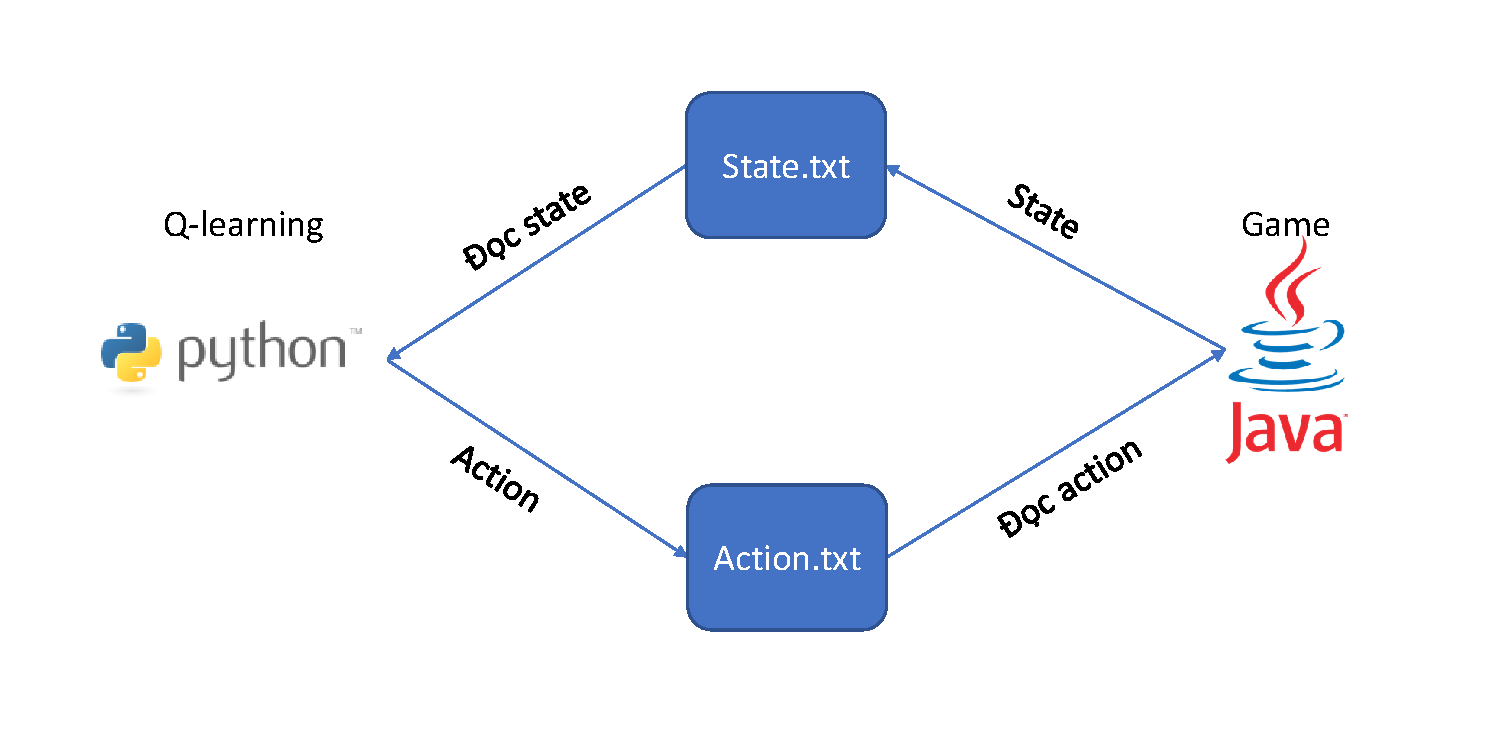
\includegraphics[width=130mm,scale=0.3]{Pic/transfer_java_env.pdf}
    \caption[Chuyển dữ liệu giữa Python và Java]{\textit{Chuyển dữ liệu giữa Python và Java}, mỗi bước thực hiện của robot được thực hiện theo thứ tự Python sẽ đọc trạng thái từ tập tin State.txt do Java cung cấp, sau đó trả về hành động được ghi vào tập tin Action.txt được Java đọc và tạo trạng thái tiếp theo.}
    \label{fig:transfer_java_env}
\end{figure}
Mô tả môi trường của World's Hardest Game (WHG) như sau:\label{begin_setting}
\begin{itemize}
    \item \textbf{Một tập trạng thái hữu hạn S}, mỗi trạng thái bao gồm vị trí của robot, vị trí của vật cản. Các vị trí này có nằm trên bản đồ kích thước 40x40.
    \item \textbf{Một tập hành động hữu hạn A},  có 5 hành động,  ($a_t=0$ : trái),  ($a_t=1$ : phải), ($a_t=2$ : lên), ($a_t=3$ : xuống), ($a_t=4$ : đứng yên).
    \item \textbf{Một hàm phần thưởng} $r = R(s_t, a_t, s_{t+1}$, đây là phần thưởng tức thời khi thực hiện hành động $a_t$: $r =1$ khi robot tới được đích, $r=-1$ khi robot đụng phải vật cản
\end{itemize}
Kiến trúc của mô hình khi chạy trên môi trường này giống giống như \cite{DBLP:journals/corr/MnihKSGAWR13} nhưng không dùng \word{Mạng nơ-ron tích chập}{Convolutional Neural Networks}.
\subsection{Môi trường Socket}
Sử dụng socket\cite{5232440} để trao đổi thông tin giữa ngôn ngữ Java và Python, với máy chủ sẽ là thuật toán Q-learning còn máy thành phần sẽ thực hiện chạy môi trường trò chơi trên Java. \\
\\
Đồng thời, nhóm tác giả đưa ra một bản đồ mới cho trò chơi, với các cài đặt đơn giản hơn, bé hơn, ít phức tạp hơn so với bản đồ gốc khi rút kinh nghiệm từ việc huấn luyện trên môi trường Java. Môi trường thay vì các bước đi của robot thay đổi theo từng pixel, chúng tôi đơn giản hóa bằng cách thay đổi mỗi bước đi sẽ theo từng ô, điều này được áp dụng cho cả vật cản. Việc cắt bớt phần vùng an toàn và vùng chiến thắng với mục đích robot sẽ "tình cờ" thắng nhiều hơn trong hình \ref{fig:1_step_new_env}
Tiến hành huấn luyện trên cả 2 môi trường trên và sử dụng kiến trúc ở môi trường Java
\begin{figure}[h]
    \centering
    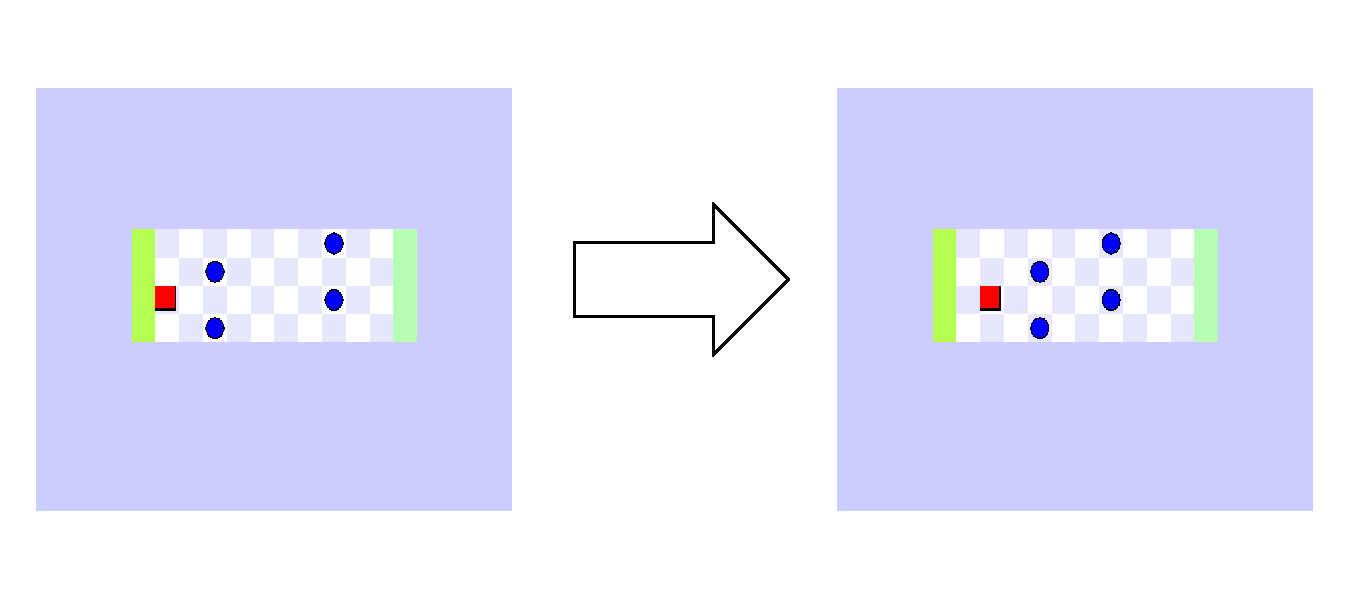
\includegraphics[width=150mm,scale=0.5]{Pic/1_step_new_env.pdf}
    \caption[Môi trường mới]{\textit{Môi trường mới}, robot thực hiện một bước (qua phải) trong môi trường mới theo từng ô thay vì từng pixel.}
    \label{fig:1_step_new_env}
\end{figure}
\subsection{Môi trường Python}
Khi môi trường lúc này của khóa luận lúc này trở nên đơn giản hơn so với môi trường gốc của WHG nên việc thực hiện lại  trò chơi trên ngôn ngữ Python không tốn nhiều thời gian. Với mục đích loại bỏ thời gian tạo hình ảnh và môi trường dễ tùy biến cho tính chất của khóa luận là điều cần thiết.\\
\section{Mô hình cơ sở}\label{baseline_model}
\subsection{Điều chỉnh trạng thái}
Khi thực hiện lại trên môi trường mới với các cài đặt như \ref{begin_setting}, nhóm tác giả thu được kết quả tệ do đó việc tìm hiểu môi trường là cần thiết. Khi xét đến vị trí hoạt động của vật cản, chúng tôi đặt ra giả thiết khi robot gặp phải trạng thái giống nhau nhưng hướng đi của các vật cản là khác nhau, sẽ khiến robot "bối rối"  được biểu thị như hình \ref{fig:conflict_enemy_position} . Do đó khi ra quyết định trên dữ kiện hiện thời sẽ phải xác định hướng đi của các vật cản mà do tính chất "không nhớ" được đề cập trong \ref{MDP} thì robot phải "đoán" khi thực hiện việc học. Để khắc phục, nhóm tác giả bổ sung hướng đi của vật cản vào các trạng thái, sẽ được mô tả cụ thể trong phần \ref{change_state}.\\
\begin{figure}[h]
    \centering
    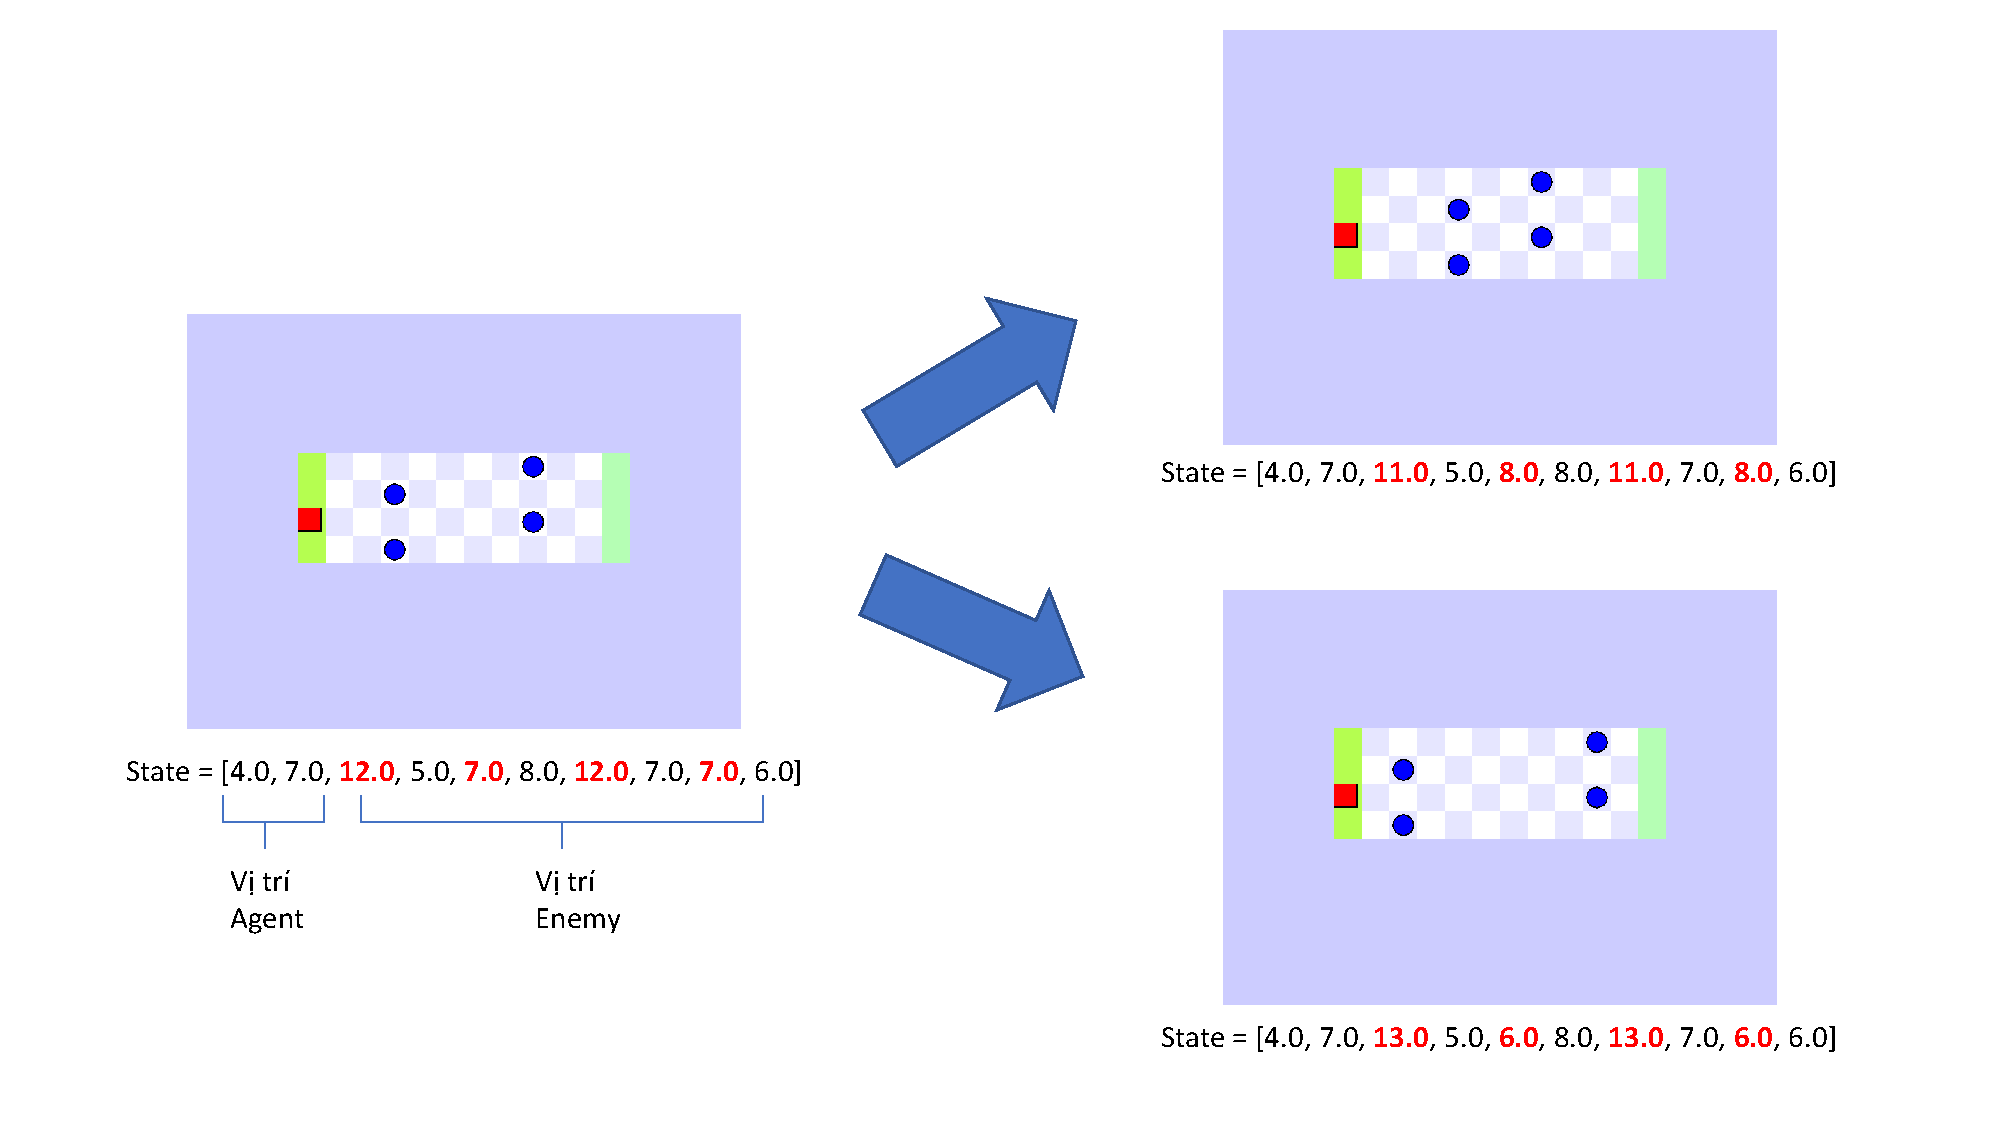
\includegraphics[width=150mm,scale=0.5]{./Pic/conflict_enemy_position.pdf}
    \caption[Đoán các trạng thái]{\textit{Đoán các trạng thái}, ví dụ của sự "rối bời" của robot khi chọn hành động giữa các sự biến đổi trạng thái. Khi gặp một trạng thái robot phải đoán bước tiếp theo của các vật cản, hình ở trên thể hiện vật cản ở vị trí hiện tại sang trái và ngược lại.}
    \label{fig:conflict_enemy_position}
\end{figure}
\subsection{Một số tùy biến tham khảo}\label{ref_app}
Sự thành công của \cite{DBLP:journals/corr/MnihKSGAWR13} là bước ngoặt trong lĩnh vực học tăng cường khi thực hiện thành công hai ý tưởng mà sau này được nghiên cứu và phát triển rất nhiều, đó là \word{Lịch sử kinh nghiệm}{Experience Replay}và \word{Mạng mục tiêu}{Target Network}.
\begin{itemize}
    \item \textbf{Lịch sử kinh nghiệm}, chứa kinh nghiệm của robot theo bộ $(s_t, a_t, s_{t+1}, r_{t+1})$. Những bộ kinh nghiệm này được lấy mẫu ngẫu nhiên trong quá trình huấn luyện nhằm cố gắng loại bỏ mối tương quan giữa các trạng thái.
    \item \textbf{Mạng Mục tiêu}, đây là bản sao của các \word{trọng số}{weights} và \word{độ nghiêng trọng số}{bias} của mô hình mỗi khi thực hiện $n$ bước. Đây sẽ là nhãn của mô hình khi thực hiện việc đánh giá quá trình hiện tại có chênh lệch quá nhiều hay không?
\end{itemize}
\subsection{Mô hình cơ sở đề xuất}
Mô hình lúc này được thiết kế vẫn như ban đầu nhưng thay thế hàm phần thưởng và trạng thái như đề cập ở trên nhằm mong muốn việc huấn luyện sẽ hội tụ nhanh hơn. Áp dụng cả phần \ref{ref_app} cùng với các cài đặt tham số được đề nghị bởi \cite{Human-level-control}.
\begin{itemize}\label{change_state}
    \item \textbf{Một tập trạng thái hữu hạn S}, trạng thái khi này được thay đổi như sau
    \begin{align}
        S_t = \left[ Pos_A(t),\quad Pos_E(t),\quad Vert(Pos_E(t))\right]
    \end{align}
    Trong đó $Pos_A(t)$ là vị trí của robot tại thời điểm t, $Pos_E(t)$ là vị trí của vật cản tại thời điểm t và $Vert(Pos_E(t))$ là hướng đi của vật cản đang xét tại thời điểm t (ở đây có 2 hướng là $True:$ trái, $False$: phải). Chú ý rằng vị trí của vật cản và hướng của vật cản là bộ ba được xếp lần lượt nhau.
    \item \textbf{Một tập hành động hữu hạn A},  có 5 hành động,  ($a_t=0$ : trái),  ($a_t=1$ : phải), ($a_t=2$ : lên), ($a_t=3$ : xuống), ($a_t=4$ : đứng yên).
    \item \textbf{Một hàm phần thưởng} $r = R(s_t, a_t, s_{t+1})$, đây là phần thưởng tức thời khi thực hiện hành động $a_t$: $r =50$ khi robot tới được đích, $r=-50$ khi robot đụng phải vật cản.
\end{itemize}
\begin{figure}[h]
    \centering
    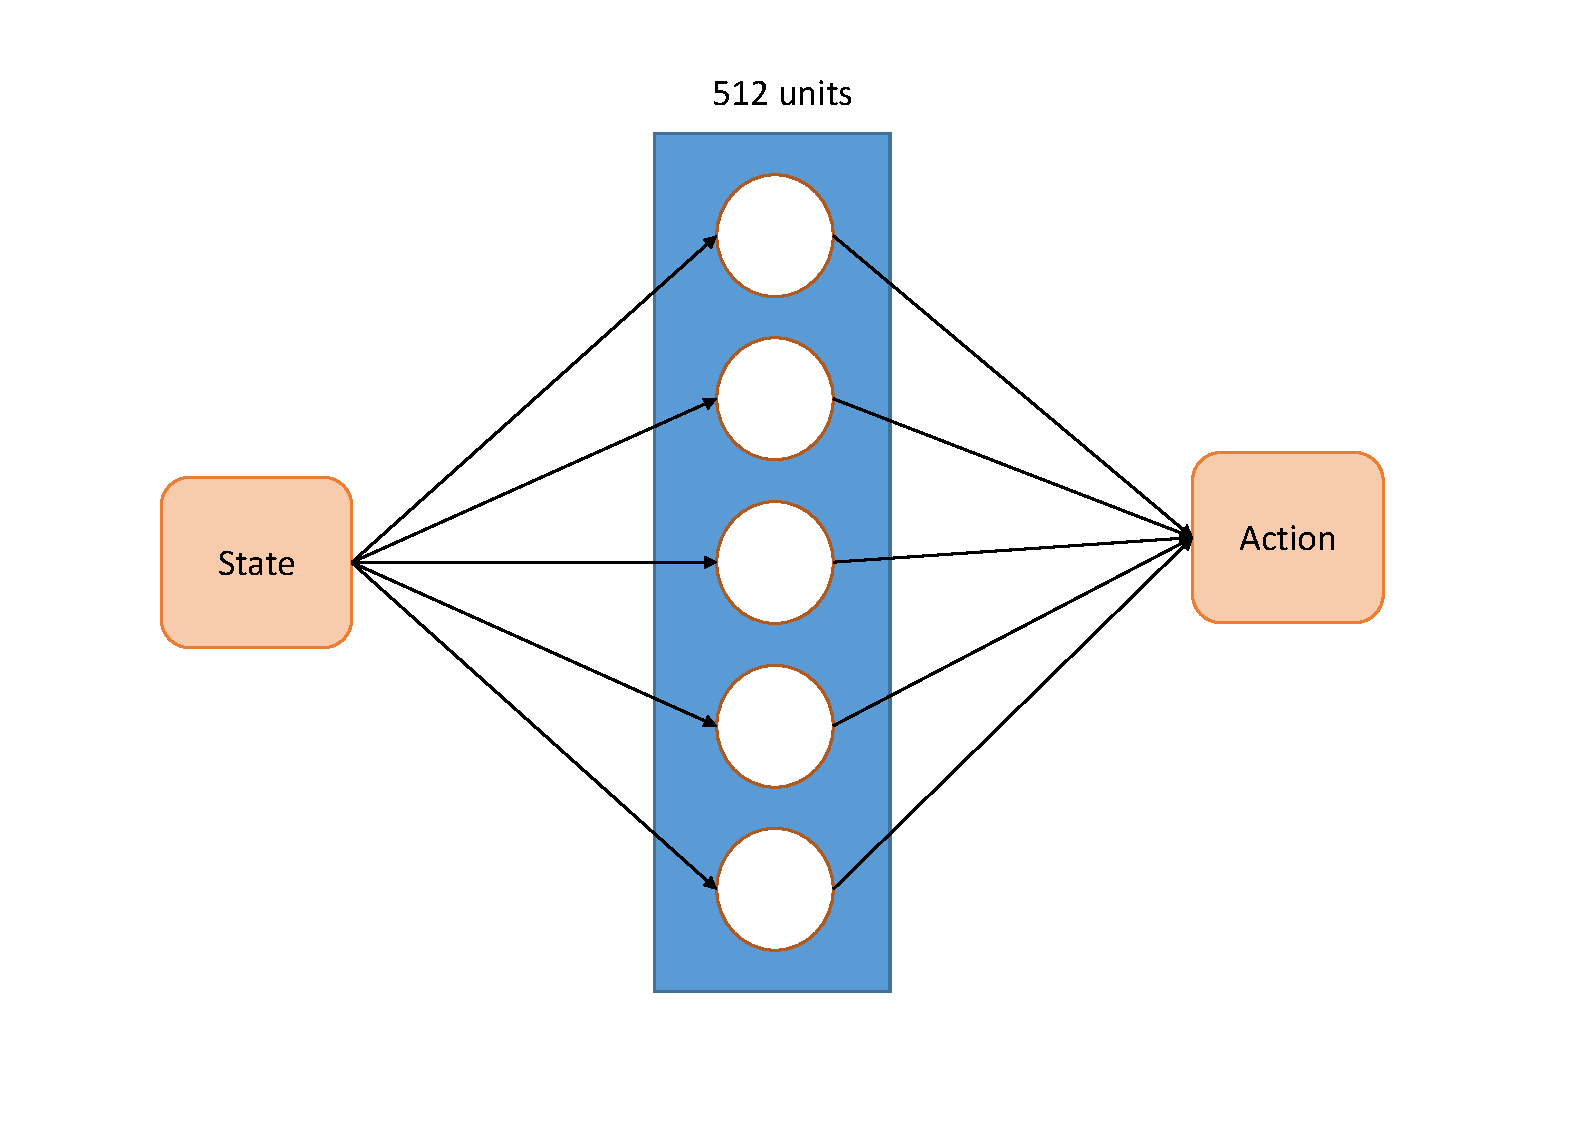
\includegraphics[height=80mm,width=140mm]{Pic/baseline/baseline_archetect.pdf}
    \caption[Cấu trúc mô hình cơ sở]{\textit{Cấu trúc mô hình cơ sở}, sử dụng một lớp ẩn để ước lượng hàm chất lượng sau khi lấy đặc trưng đã được phân tích trước đó.}
    \label{fig:baseline_archetect}
\end{figure}
Nhóm tác giả sử dụng cấu trúc như hình \ref{baseline_model} được lấy ý tưởng từ \cite{DBLP:journals/corr/MnihKSGAWR13} khi trực tiếp thực hiện \word{Phân tích đặc trưng}{Feature Extraction}thay vì sử dụng CNN.
\vspace{1cm}
\section{Một số thử nghiệm được thực hiện}
\noindentÝ tưởng đơn giản nhất cho việc tối ưu các bước thực hiện trong mỗi tập là thay đổi hàm phần thưởng thành một lượng âm. Khi đó, lượng phần thưởng âm này sẽ thúc đẩy robot mau chóng thắng nhưng nhóm tác giả có thể tiên lượng rằng robot sẽ không muốn tồn tại lâu trên bản đồ (thực hiện "kết liễu" càng nhanh càng tốt). Vì vậy giới hạn số bước có thể thực hiện trong một tập cũng là bước thử nghiệm trong phần này.\\
\\
Ngoài ra, khi hàm mất mát \ref{fig:baseline_loss} khá ổn định nhưng trung bình tích lũy \ref{fig:baseline_avg} không tăng tuyến tính như mong muốn. Chúng tôi giả thiết rằng bước khám phá chưa đủ đối với bài toán cụ thể này, do đó hai ý tưởng được đề xuất là tăng thêm số lượng bước thực hiện khám phá môi trường và tự tạo trạng thái tức ngẫu nhiên vị trí của robot và vị trí của vật cản.
\clearpage
\subsection{Mô hình đầu tiên}
\label{first_model}
Thực hiện các ý tưởng được nói ở trên, chúng tôi đề xuất các thay đổi cho mô hình mới như sau:
\begin{itemize}
    \item \textit{Thay đổi hàm phần thưởng:} Không chỉ sử dụng hai giá trị như mô hình cơ sở, chúng tôi xét môi trường robot hoạt động với mong muốn sẽ có một lượng phần thưởng âm khi robot đến càng gần điểm đích:
    \begin{subnumcases}{r(s_t,a_t,s_{t+1})=}
        +R_{0} & $s_{t+1}=\text{đích}$ \\
        -R_{1} & $s_{t+1}=\text{chết}$\\
        -d(s_{t+1}) & còn lại\label{first_subtract}
    \end{subnumcases}
    Với $R_0$ và $R_1$ là hằng số và hàm $d(s_{t+1})$ chỉ thị cho mối tương quan giữa trạng thái tiếp theo đến các vùng kết thúc, nhóm tác giả sử dụng ở đây là:
    \begin{equation}
        d(s_{t+1}) = \frac{\text{vị trí cột đích}-\text{vị trí cột trạng thái tiếp theo}}{\text{\text{vị trí cột đích} - \text{vị trí cột bắt đầu}}}
    \end{equation}
    Sở dĩ công thức \ref{first_subtract} phải trừ đi lượng\textit{ vị trí cột đích - vị trí cột bắt đầu} vì khi để giá trị cao quá sẽ khiến cho robot không còn muốn tồn tại trên bản đồ. Với cách định nghĩa như trên, nhóm tác giả mong muốn robot sẽ nhận biết được càng đến gần đích thì sẽ trừ càng ít và càng sử dụng nhiều số bước sẽ càng bị phạt.
    \item \textit{Thay đổi các khám phá môi trường:} Việc thử hiện hành động ngẫu nhiên theo chiến thuật \ref{e-greedy} dường như không đủ trường hợp thắng để robot có thể nhận biết được môi trường hiện tại có thể thắng hay không. Hình \ref{fig:agent_pos} đầu tiên cho thấy rằng rất khó để robot có thể vượt qua được các cột đầu tiên của môi trường và chiến thắng là điều trăn trở. Chứng tỏ đây là môi trường nhỏ rất dễ bước vào trạng thái kết liễu, do đó việc robot chỉ ngẫu nhiên thực hiện các bước có thể gói gọn trong vùng gần an toàn. Nhóm tác giả đề xuất thực hiện khởi tạo ngẫu nhiên vị trí của robot và vật cản để các trường hợp có thể gặp đa dạng hơn, từ đó có thể học được tốt hơn.
    \item \textit{Thay đổi cấu trúc của mô hình:} Thay vì sử dụng lớp ẩn 512 phần tử, mô hình mới chỉ sử dụng lớp ẩn 64 phần tử. Vì trạng thái hiện tại của môi trường rất nhỏ chỉ 14 giá trị do đó việc sử dụng lớp ẩn quá lớn là không cần thiết.
\end{itemize}
\begin{figure}[ht]
    \centering
    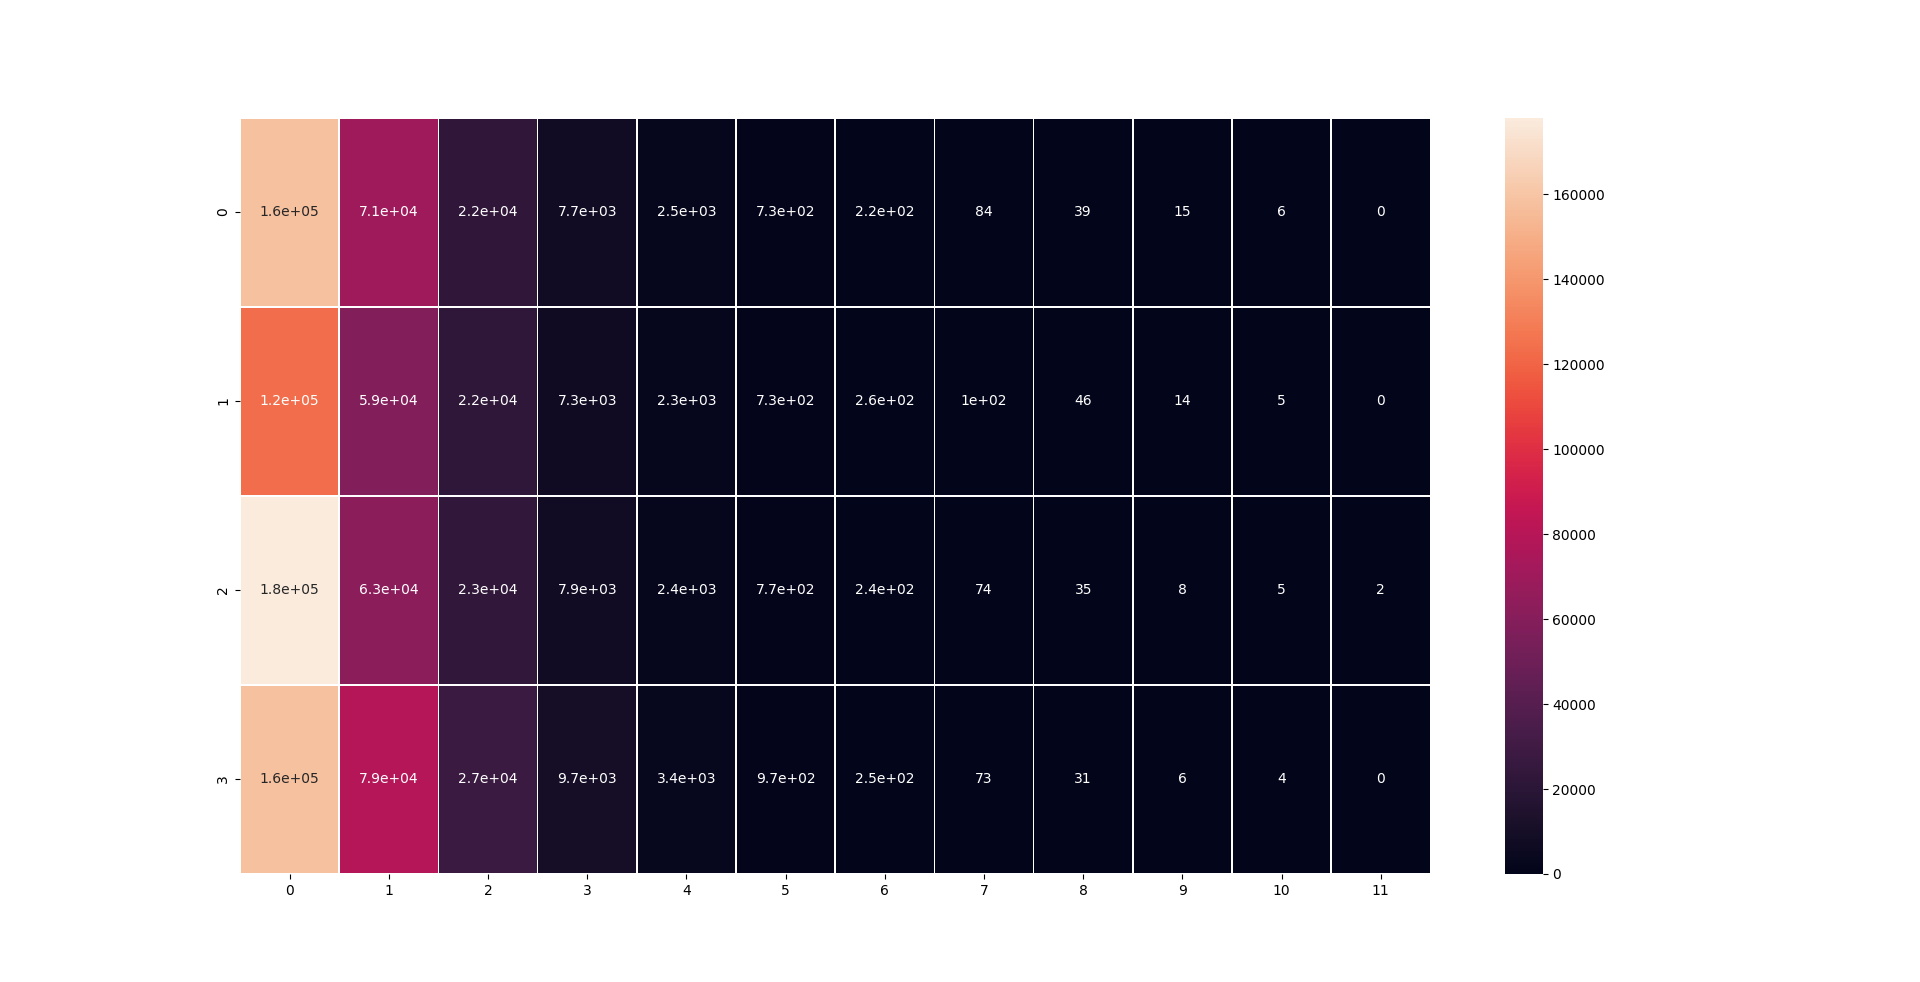
\includegraphics[width=1.2\linewidth]{Pic/First_model/agent_pos_before.png}
    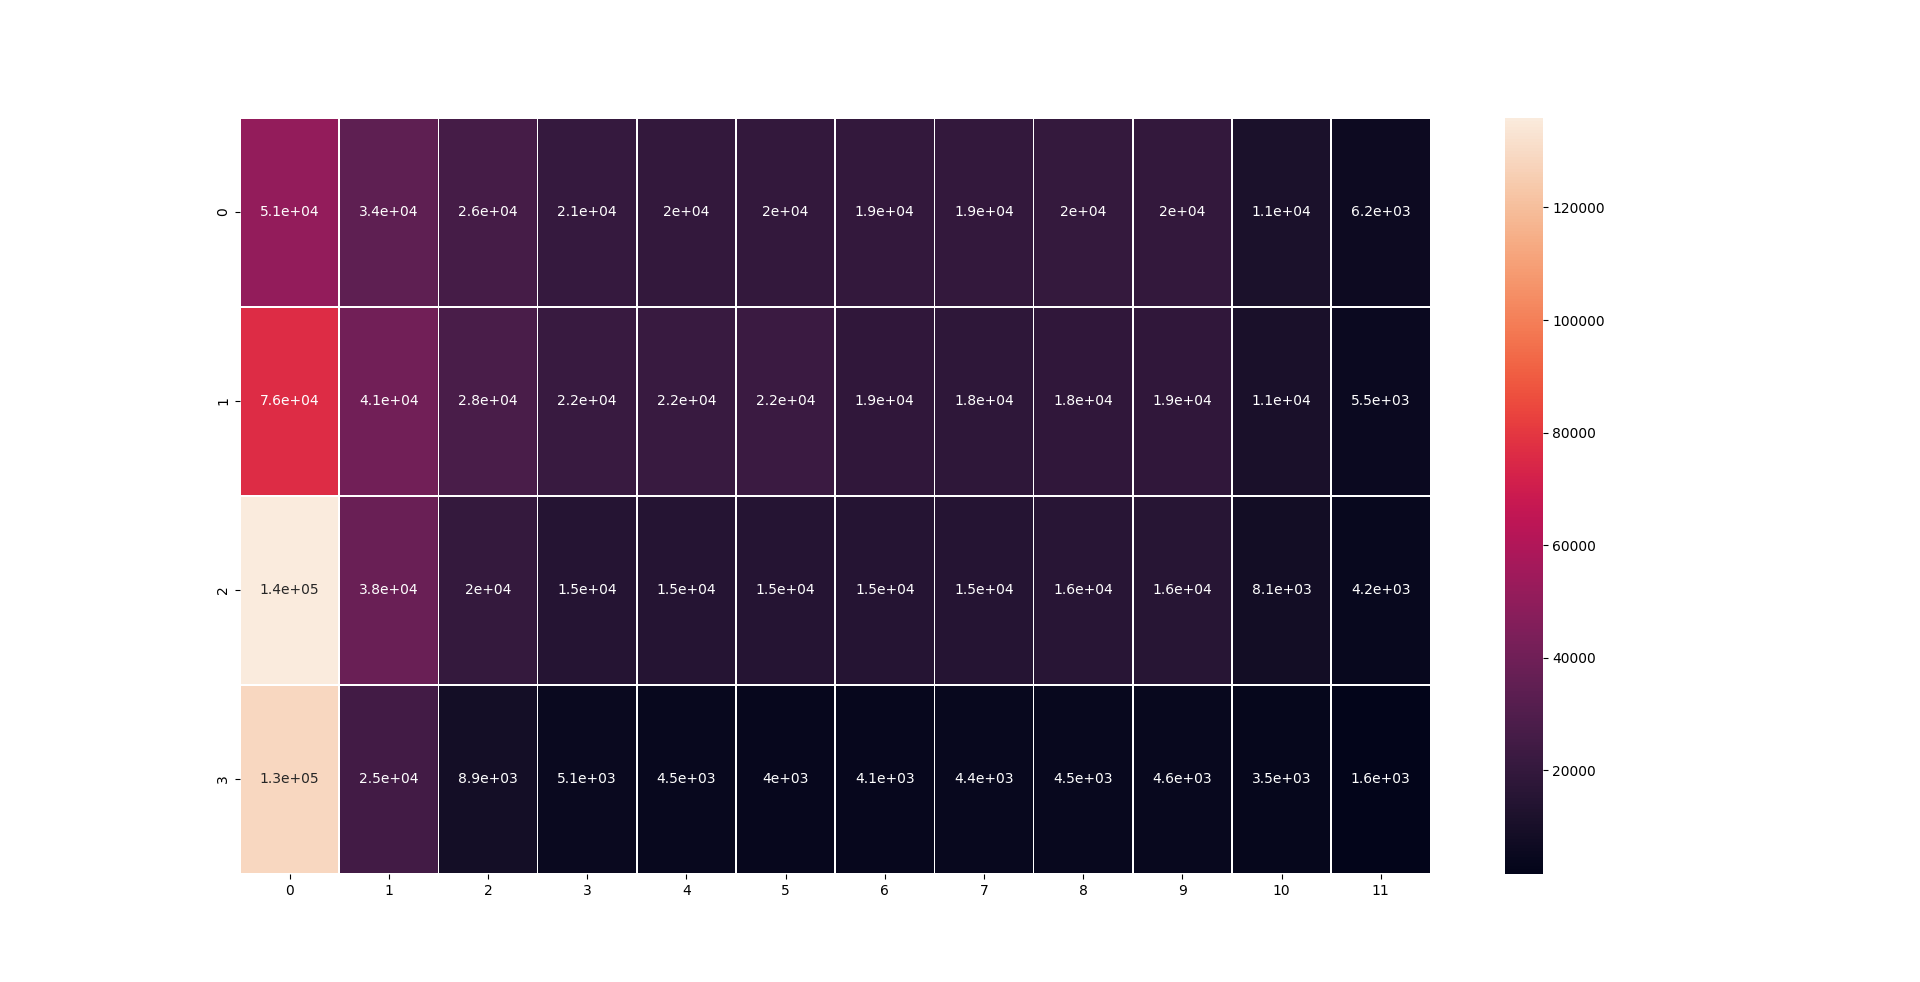
\includegraphics[width=1.2\linewidth]{Pic/First_model/agent_pos_after.png}
    \caption[Bản đồ nhiệt các vị trí robot thường xuất hiện]{Đây là kết quả của thử nghiệm chạy 1M bước ngẫu nhiên robot có thể đi được trong môi trường. Hình đầu tiên là kết quả không ngẫu nhiên vị trí robot, còn hình thứ hai là thực hiện khám phá môi trường khi ngẫu nhiên vị trí của các vật thể trong bản đồ. Có thể thấy được rằng các vị trí gần đích robot đã đi nhiều hơn từ đó tạo các dữ liệu thắng
    hơn cho mô hình.}
    \label{fig:agent_pos}
\end{figure}
\clearpage
\subsection{Mô hình thứ 2}\label{second_model}
Sau khi không có cải thiện trong mô hình \ref{first_model}, nhóm tác giả đưa ra giả thiết rằng các đặc trưng hiện tại khi đưa vào Q-learning chưa đủ liên quan với nhau để mô hình có thể nhận biết được tốt chúng. Ngoài ra các hàm mất mát của các kết quả \ref{first_model:first_try} và \ref{first_model:second_try} tuy có thể "hội tụ" nhưng đồ thị đồ thị phần thưởng tích lũy không tăng lên, có thể khẳng định rằng mô hình đã tìm đến điểm "cận cực đại" để khắc phục vấn đề này chúng tôi sử dụng \word{Công cụ tối ưu}{Optimizer}khác. 
\begin{itemize}
    \item \textit{Thay đổi cấu trúc của mô hình:} Từ 1 lớp ẩn 64 chúng tôi sử dụng 2 \word{Lớp ẩn}{Hidden layer} 64 nhằm giúp mô hình học được sự phức tạp của môi trường.
    \item \textit{Thay đổi công cụ tối ưu:} Nhóm tác giả thực hiện thay đổi từ RMSprop sang Adam.
    \item \textit{Thay đổi kích thước \word{cụm dữ liệu}{batch}:}  Theo  \cite{DBLP:journals/corr/abs-1803-02811}, sử dụng batch trong khoảng từ $32-2048$ là hợp lý đối với Q-learning. Do đó, chúng tôi lấy kết quả tốt nhất được thử nghiệm là 512 để thực hiện vào mô hình.
\end{itemize}
\begin{figure}[h]
    \centering
    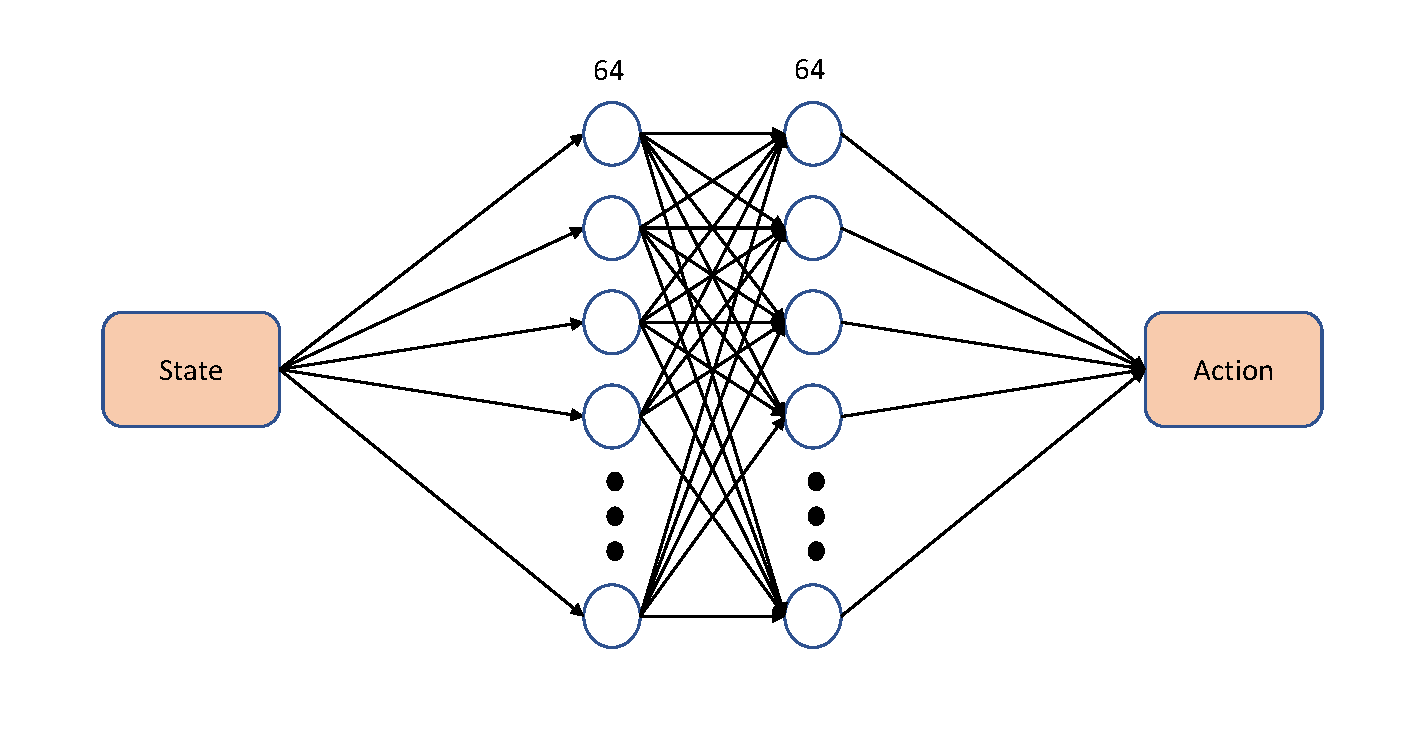
\includegraphics[width=\linewidth]{Pic/Second_model/second_arch.pdf}
    \caption[Cấu trúc của mô hình thứ hai]{\textit{Cấu trúc của mô hình thứ hai}, mô hình thêm một lớp ẩn nhằm thay đổi cách lớp ẩn thứ 2, tức Q-learning, nhìn vào trạng thái của môi trường.}
    \label{fig:second_arch}
\end{figure}


\chapter{Kết quả và thảo luận}\label{Chap4}
\section{Chuẩn bị môi trường}
\label{env_repair_result}
Trong phần này, nhóm tác giả sẽ thực hiện huấn luyện trên các môi trường trong phần \ref{env_repair} và đưa ra kết luận như sau:
\begin{enumerate}
    \item \textbf{Môi trường Java}\\
    Việc huấn luyện trên môi trường Java rất chậm chỉ khoảng 20 trạng thái được truyền đi trong 1 giây khi robot khám phá môi trường. Mặc dù đã dùng trạng thái khác so với hình ảnh trong \cite{WHG_yasyf} nhưng kết quả vẫn không khả quan. Robot không thể học được cách thoát ra khỏi vùng an toàn. Việc khám phá để thoát ra khỏi vùng an toàn chiếm khá nhiều bước nên để robot "tình cờ" thắng trong trò chơi là rất khó.
    \begin{itemize}
        \item \textit{Ưu điểm:} rất dễ thực hiện khi ở các bước ban đầu của khóa luận. Không cần can thiệp nhiều vào code nguồn.
        \item \textit{Khuyết điểm:} Vì đây là trò chơi được viết trên Java Swing nên khi huấn luyện việc tạo hình ảnh là điều không thể tránh khỏi. Việc lãng phí tài nguyên cho hình ảnh khiến cho chương trình chạy rất chậm mặc dù nhóm đã nghiên cứu về các phương pháp giúp không tạo hình ảnh khi chạy như \cite{ghostawt} hay \cite{headlessjavase} nhưng không thể thực hiện
        do mã nguồn không đáp ứng yêu cầu của các công cụ trên.
    \end{itemize}
    \textit{Kết luận:} Cần có sự cải thiện trong việc truyền dữ liệu giữa ngôn ngữ Java và Python. Nếu bước khám phá của robot chỉ có thoát ra khỏi vùng an toàn và bị hạ gục sẽ làm cho các bước khám phá chỉ làm cho robot "rụt rè" hơn. 
    \item \textbf{Môi trường Socket}\\
    Khả năng huấn luyện ảnh hưởng bởi việc truyền thông tin rất nhiều khi tốc độ được cải thiện, khoảng 100 trạng thái được truyền đi trong 1 giây khi robot khám phá môi trường với bản đồ gốc của WHG và 500 trạng thái đối với môi trường mới.\\
    Sau hơn 1 tuần huấn luyện trên môi trường gốc, chúng tôi không thu được kết quả khá quan nên không có kết quả để báo cáo nhưng với môi trường mới, kết quả mang lại nhiều hứa hẹn.\\
    \\
    \textit{Kết luận:} Đã có bước cải thiện tốc độ rõ rệt trong quá trình huấn luyện, điều này giúp nhanh nắm bắt được các robot phản ứng với môi trường hơn để dễ tùy biến hơn.\\
    Chương trình vẫn giữ môi trường Java của trò chơi nên các bước huấn luyện sẽ kèm thêm thời gian tạo hình ảnh của \word{Máy ảo Java}{JVM}\cite{stark2012java} do đó thời gian huấn luyện của trò chơi có thể được cải thiện  hơn nữa.\\
    Kết quả huấn luyện trên hai môi trường không thỏa mãn kỳ vọng cũng như mục tiêu của khóa luận này tuy nhiên nhóm tác giả chọn môi trường mới làm mục tiêu mới để nghiên cứu và phát triển trong tương lai vì có những chuyển biến tích cực.\\
\end{enumerate}
\section{Mô hình cơ sở}
Chúng tôi đưa ra kết quả sau khi huấn luyện xong mô hình cơ sở với 10M được thực hiện (khoảng gần 500,000 tập). Dựa trên hình \ref{fig:result_baseline}, ta có thể thấy robot có thể học được môi trường hiện tại khi có rất nhiều trường hợp thắng nhưng quan trọng là hàm tích lũy không tăng tuyến tính.\\
Tuy vậy đồ thị \ref{fig:baseline_avg} cho thấy rằng robot chưa tìm được chính sách để có thể thắng với mọi trường hợp có thể có bằng chứng có thể thấy hàm mất mát \ref{fig:baseline_loss} không hội tụ.\\
\clearpage
Ngoài ra, đồ thị \ref{fig:baseline_step} biểu thị các bước trong các bước robot thực hiện trong từng tập  có thể thấy rằng đa số đều rất nhiều, nhiều nhất lên đến hơn 3000 bước, điều này không đúng với mục tiêu của khóa luận.\\
Lưu ý rằng, đồ thị của giá trị Q tăng lên cực đại, sau đó lại giảm và giữ đều ở giá trị 30 trong một khoảng thời gian dài. Nhóm tác giả cho rằng khi sau khi đạt cực đại robot gặp rất nhiều trạng thái khác và chính sách tại đỉnh cao nhất không thỏa mãn được chúng.\\
Chúng tôi có thể khẳng định rằng mô hình hiện tại có thể tìm được đường đi giúp robot thắng được khi tỉ lệ thắng \footnote{Nhóm tác giả đã thực hiện 1000 vòng chơi với các trọng số đã được huấn luyện và môi trường ban đầu với 5 bước đầu tiên đi ngẫu nhiên} đạt \textbf{16.0\%}, tuy nhiên tối ưu số bước thực hiện và thắng được tất cả trạng thái là nhiệm vụ chính của các cải tiến tiếp theo trong khóa luận.
\begin{figure}[ht]
    \centering
    \begin{subfigure}{.5\textwidth}
      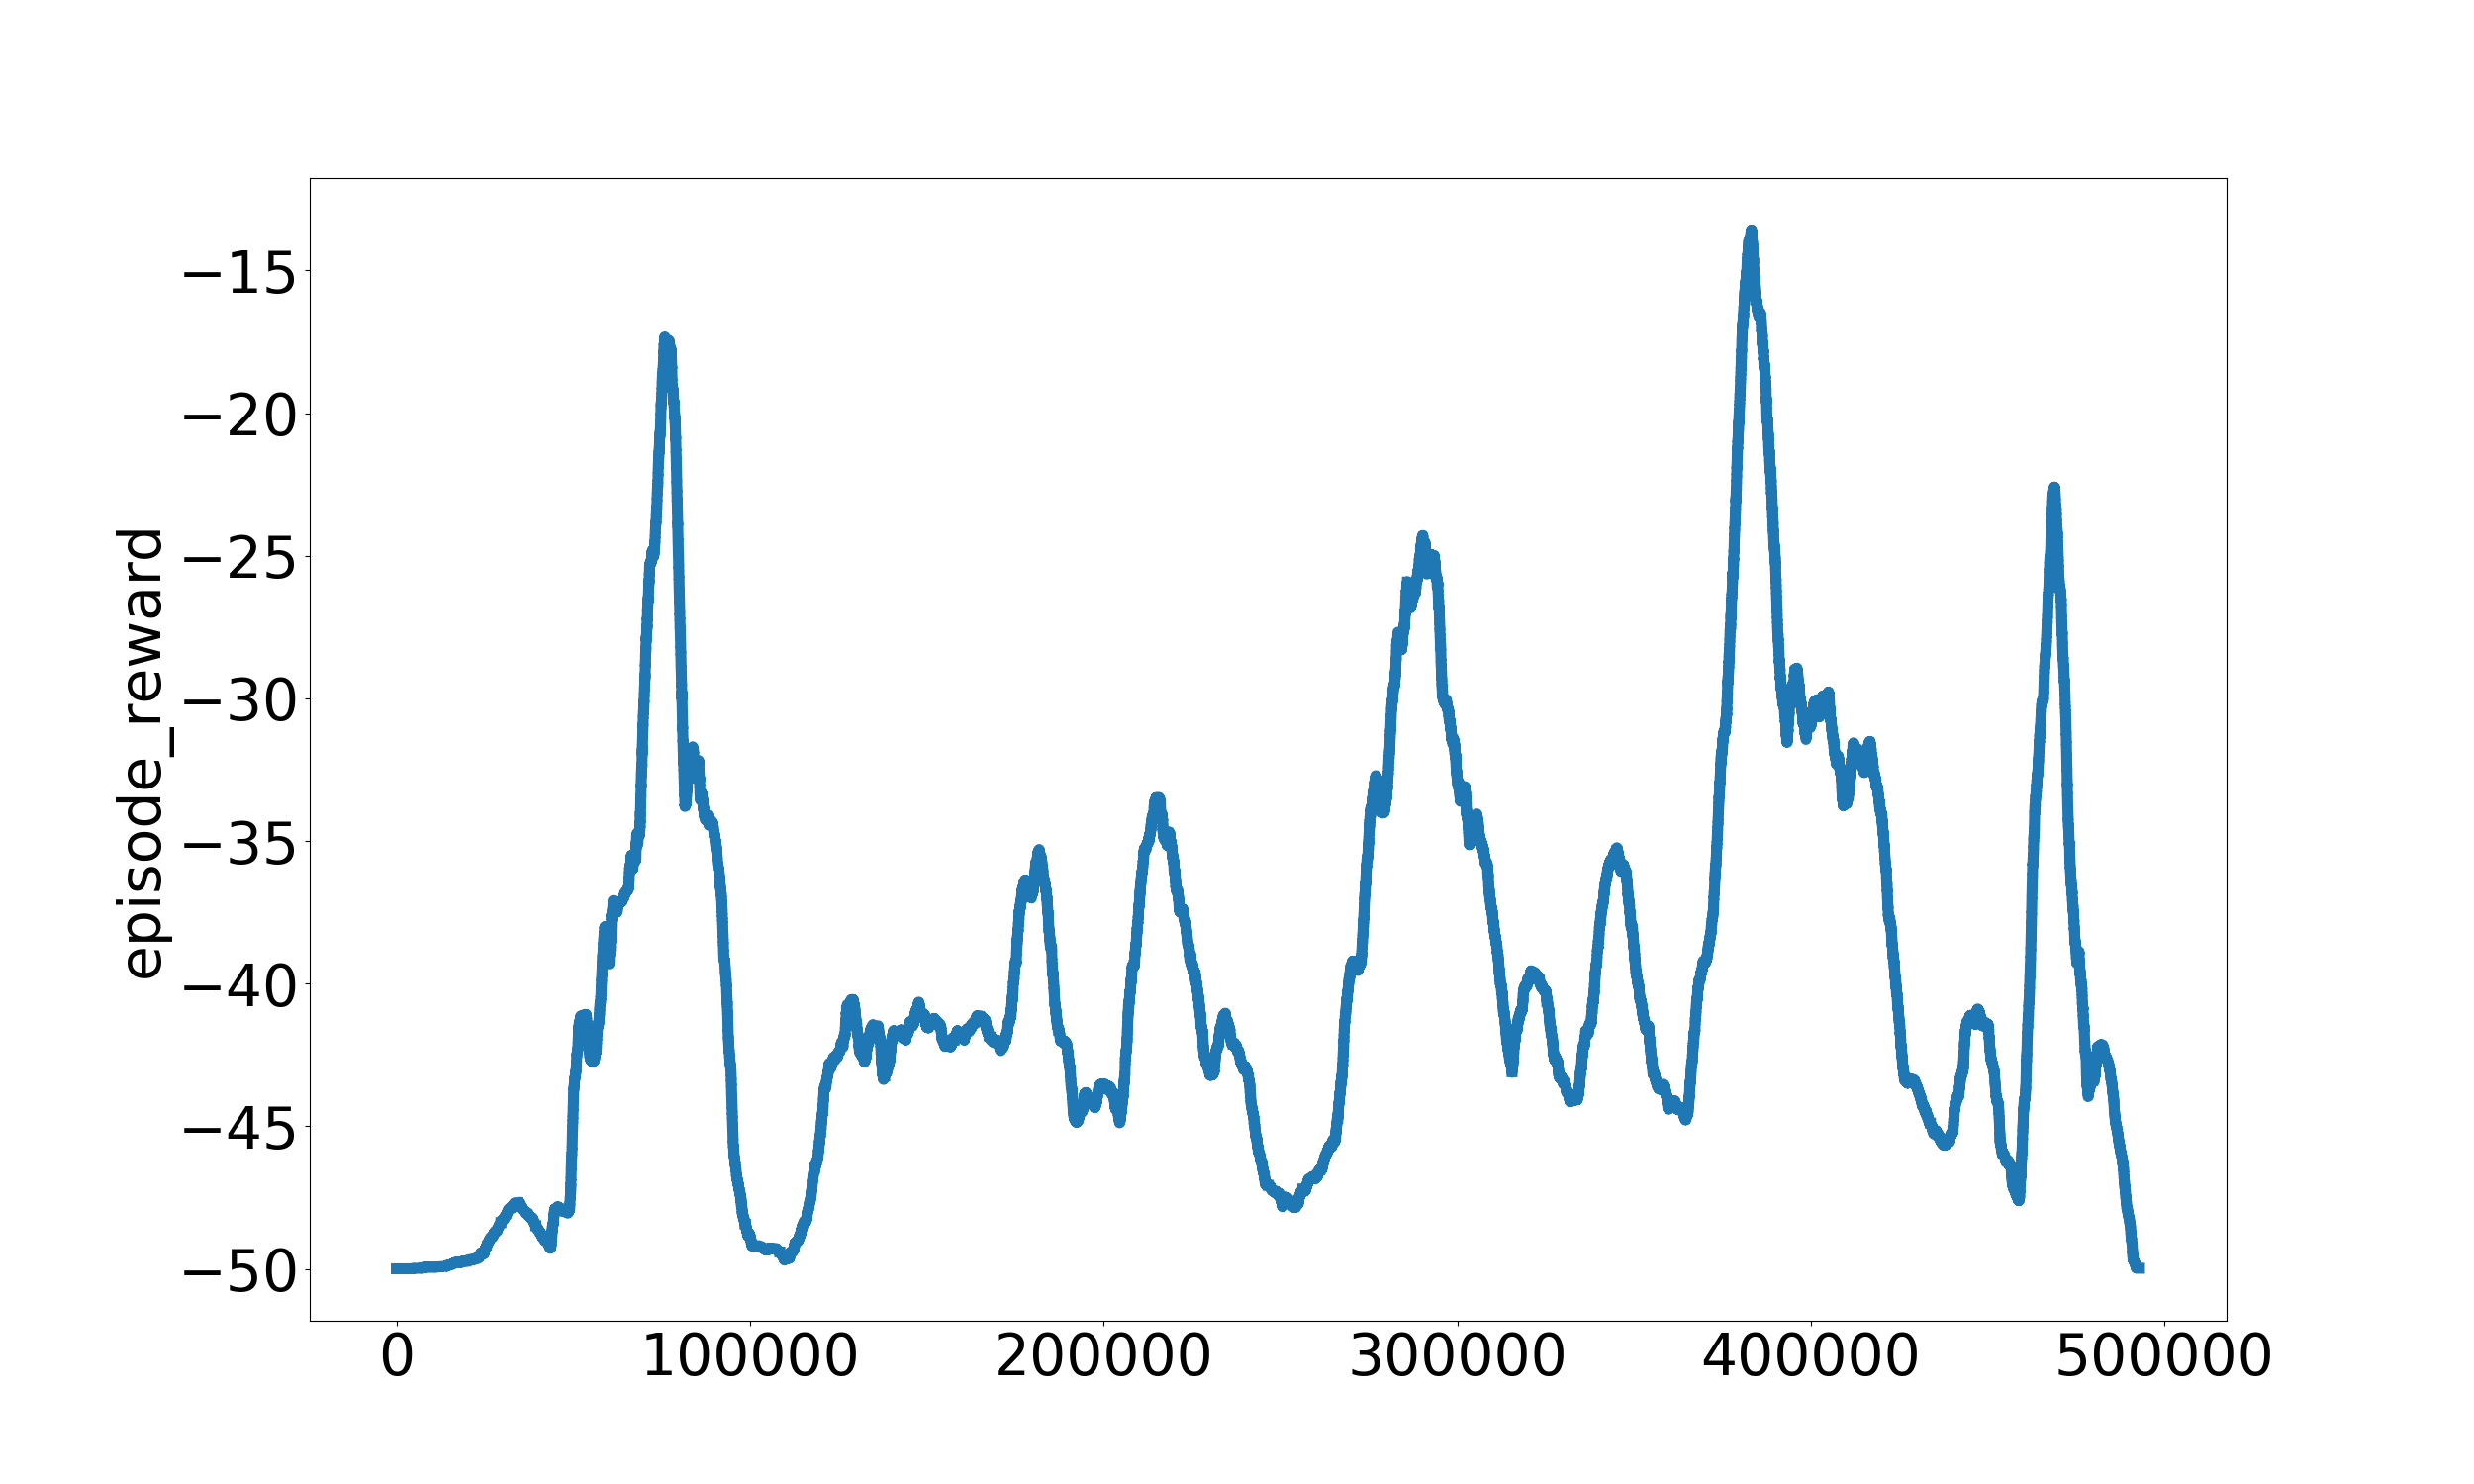
\includegraphics[width=1.1\textwidth]{Pic/baseline/episode_reward.png}  
      \caption{Trung bình tích lũy phần thưởng}
      \label{fig:baseline_avg}
    \end{subfigure}%
    \begin{subfigure}{.5\textwidth}
      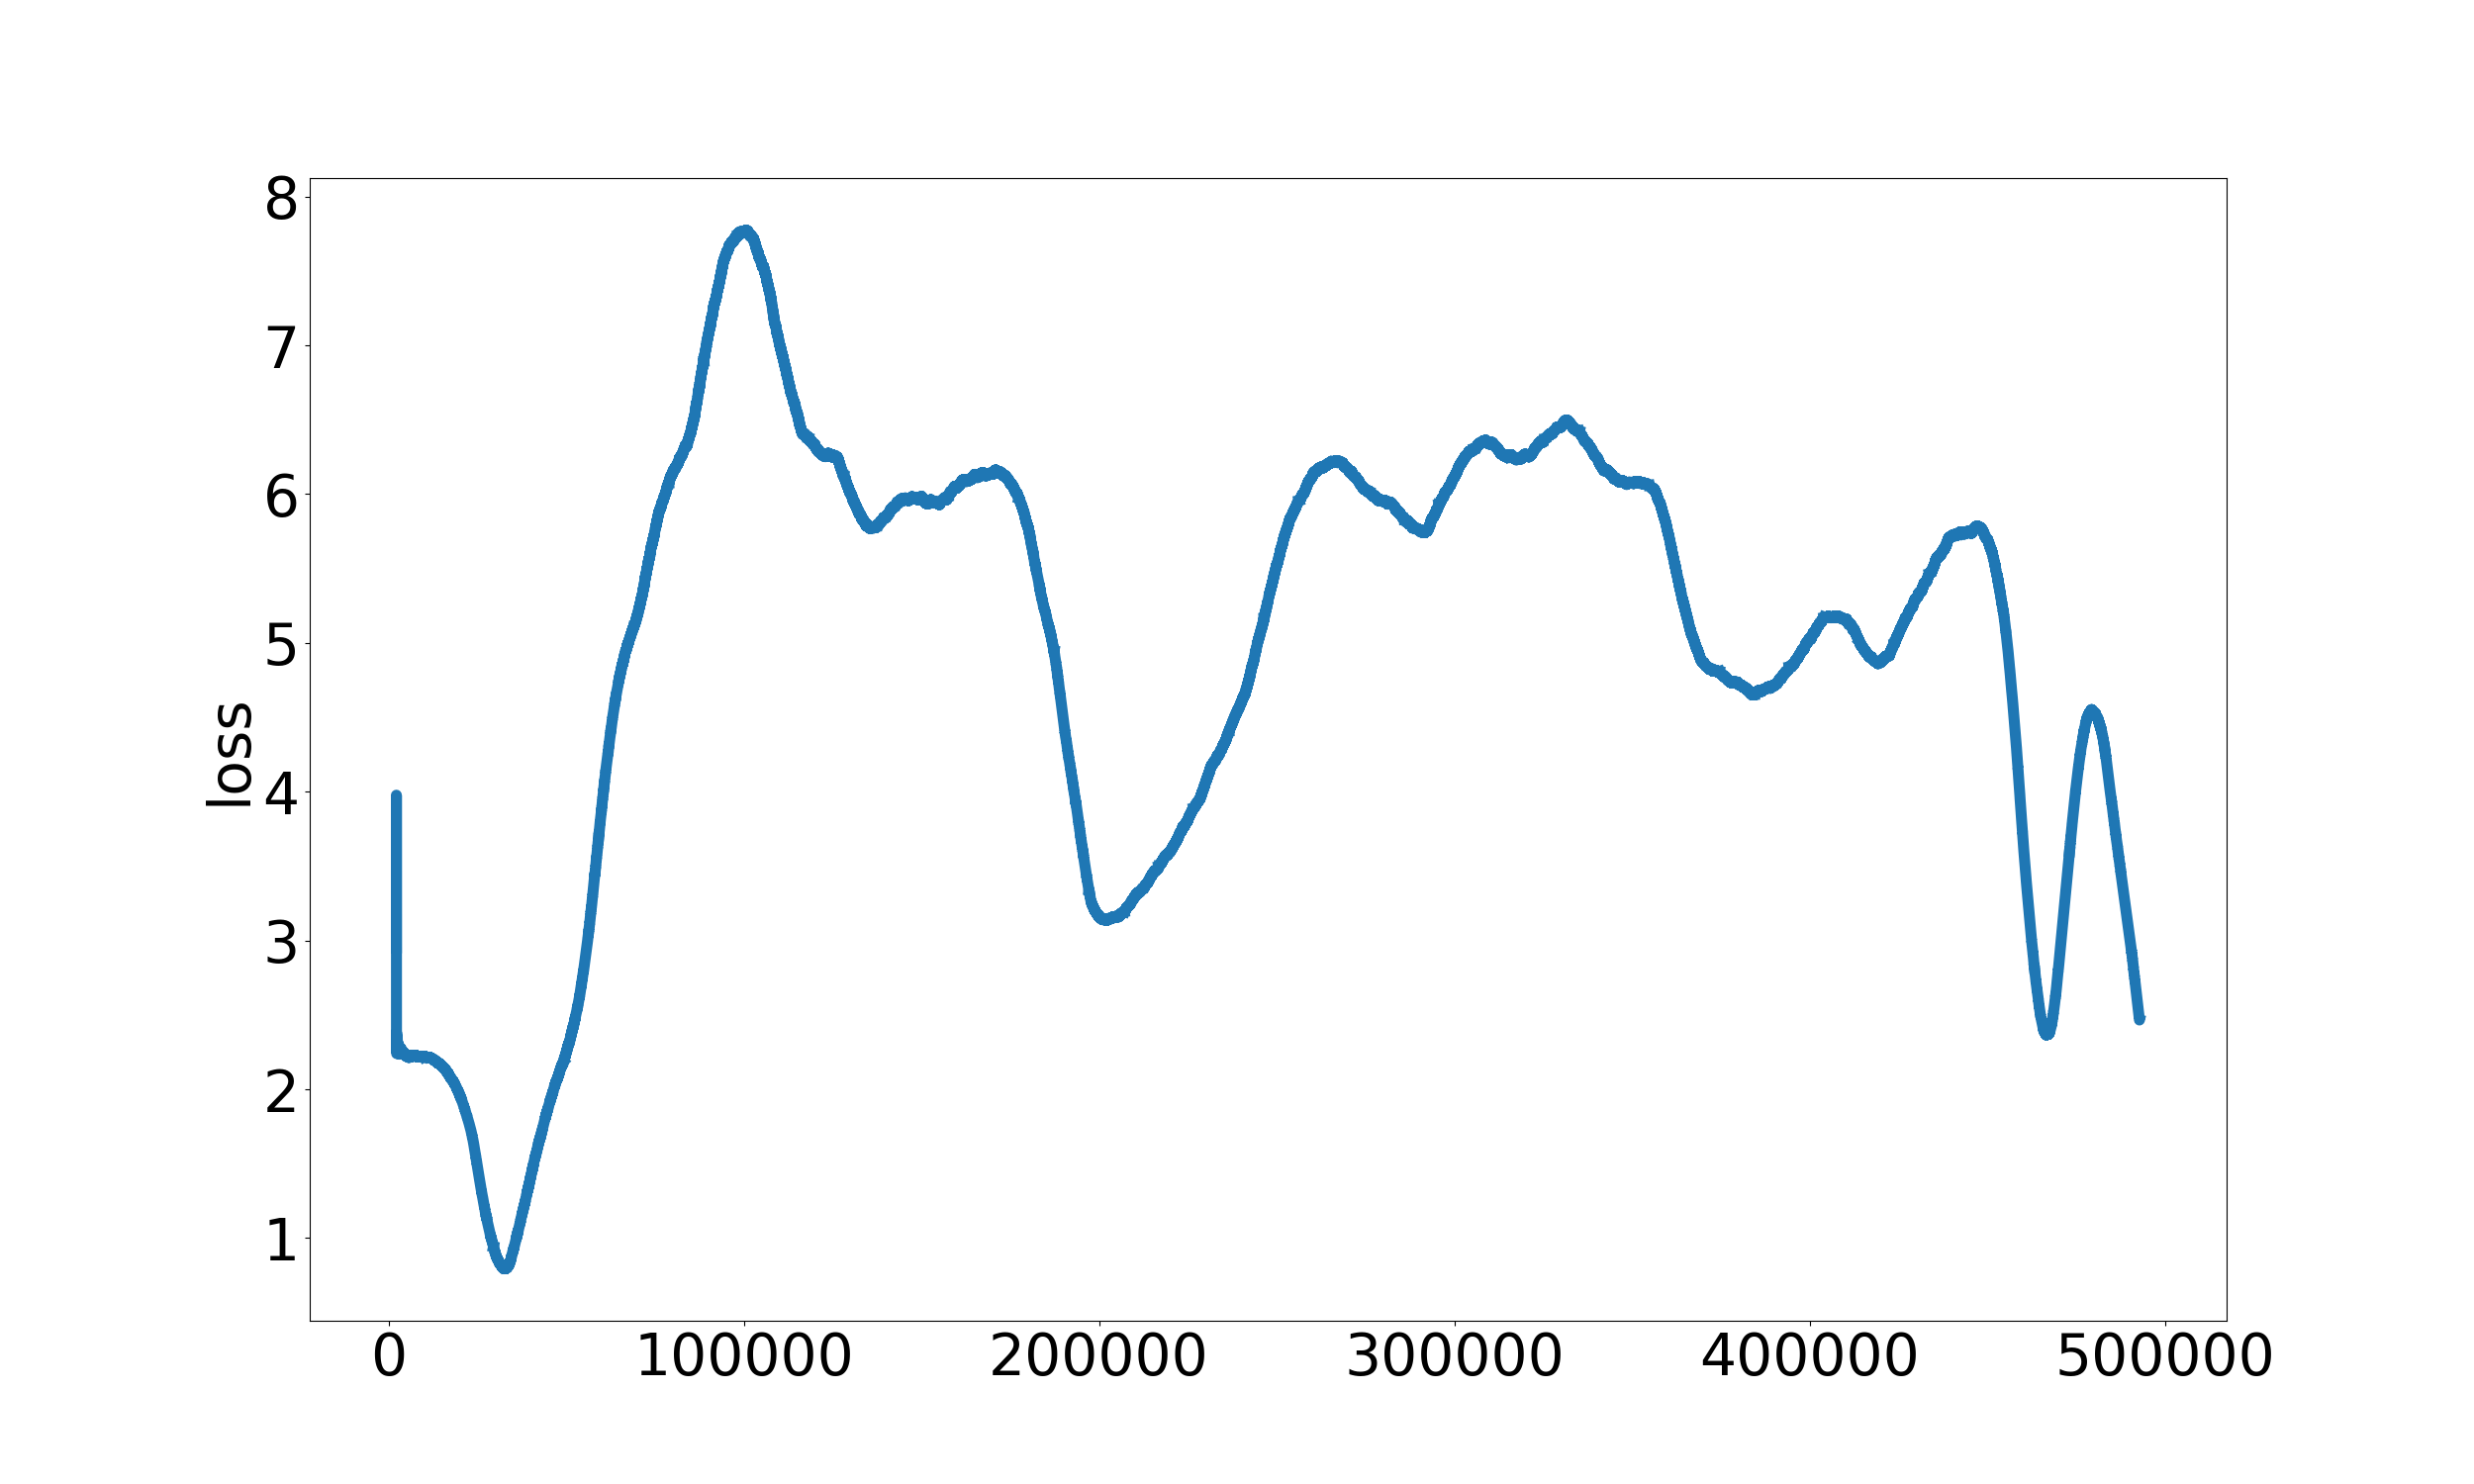
\includegraphics[width=1.1\textwidth]{Pic/baseline/loss.png}  
      \caption{Hàm mất mát}
      \label{fig:baseline_loss}
    \end{subfigure}\\
    \begin{subfigure}{.5\textwidth}
      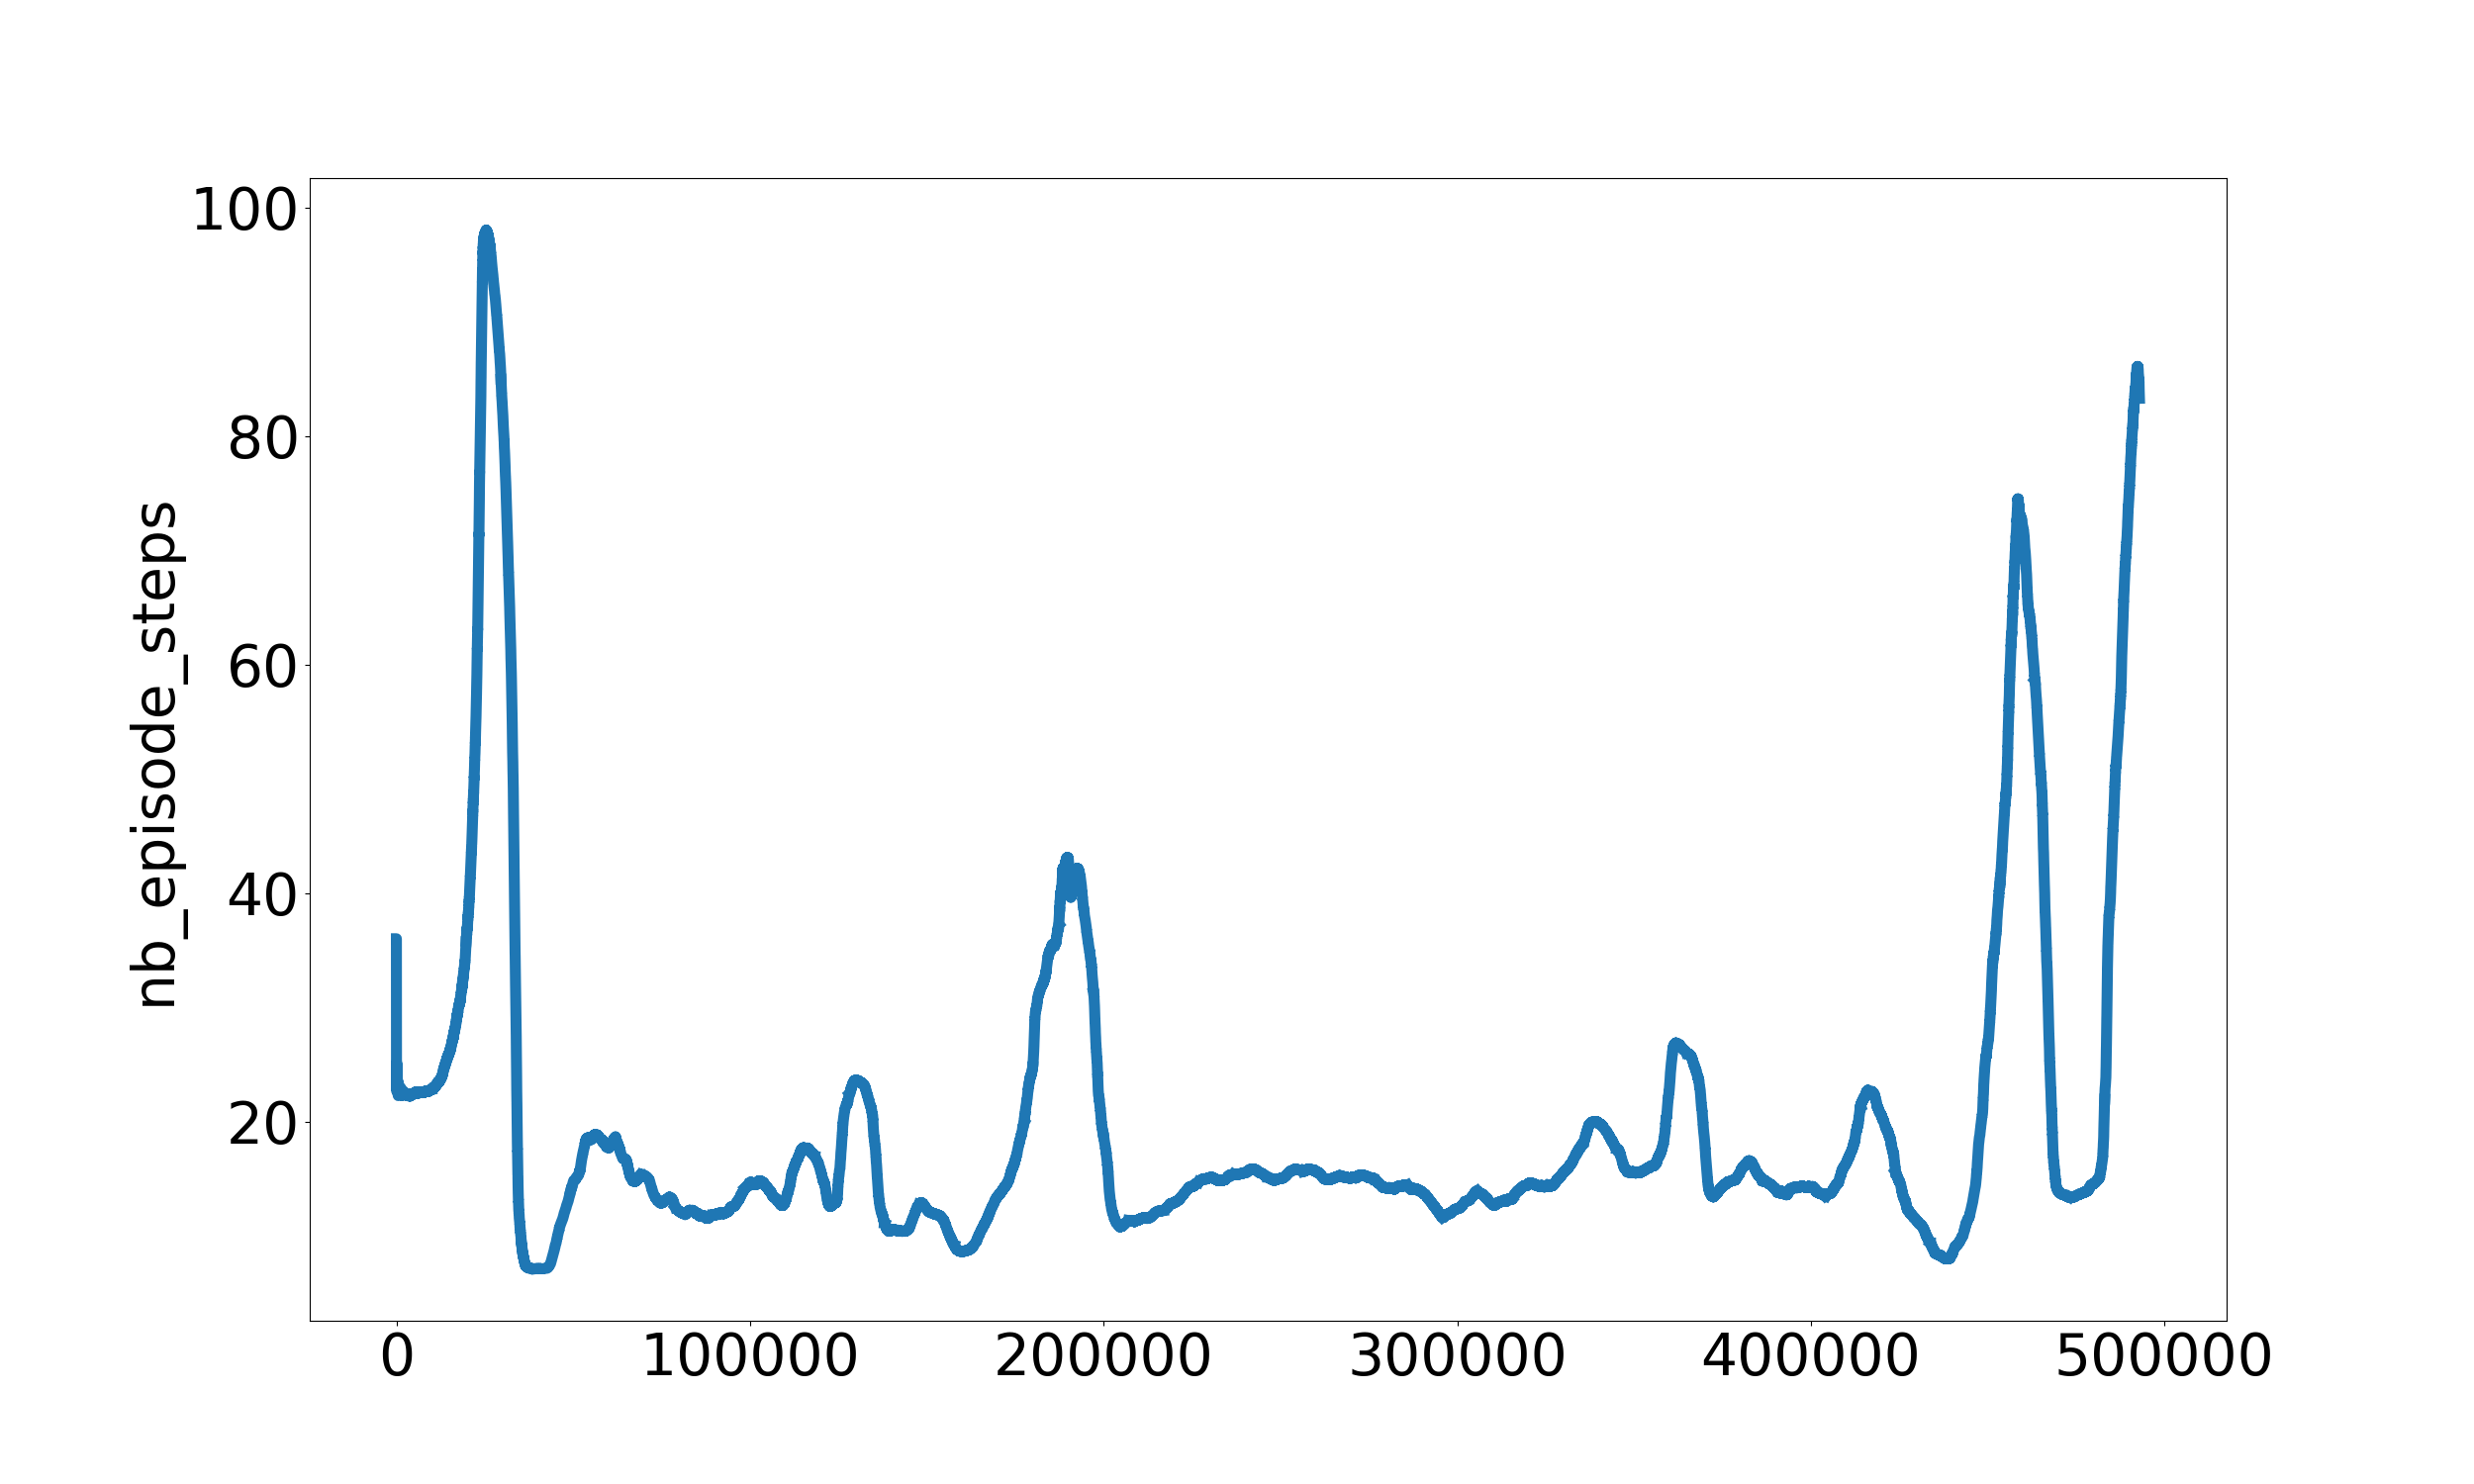
\includegraphics[width=1.1\textwidth]{Pic/baseline/nb_episode_steps.png}
      \caption{Số bước thực hiện}
      \label{fig:baseline_step}
    \end{subfigure}%
    \begin{subfigure}{.5\textwidth}
      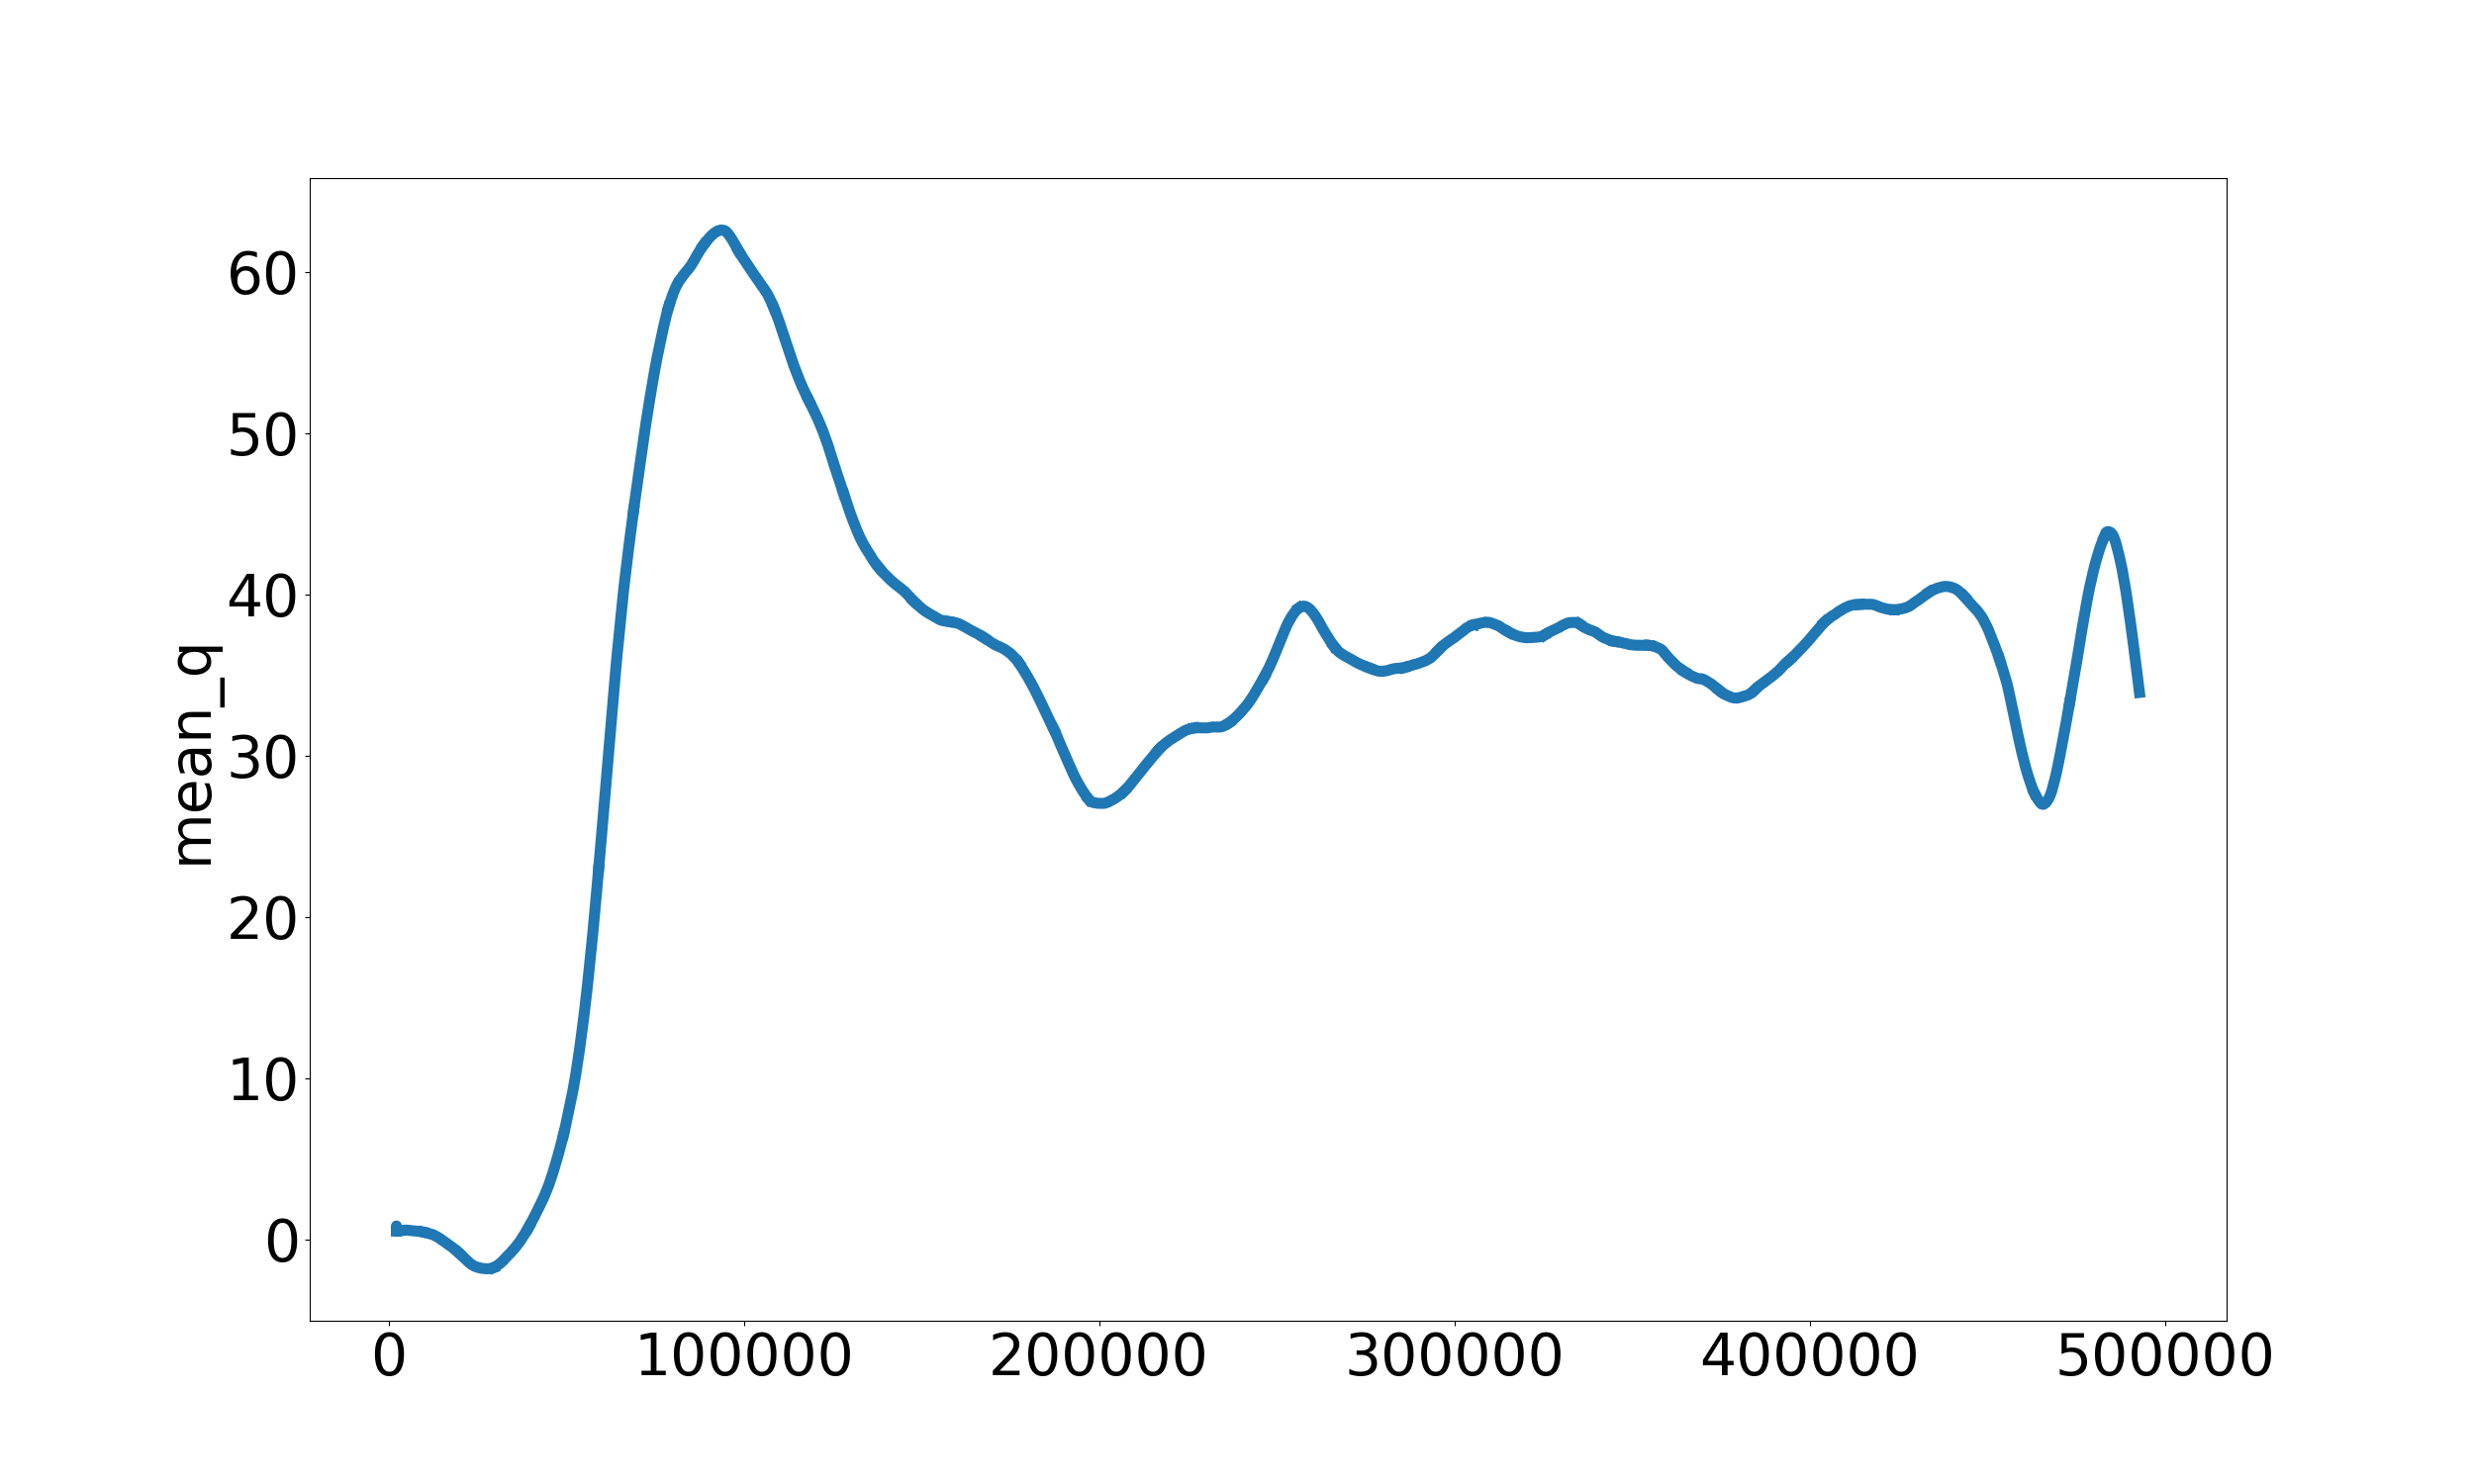
\includegraphics[width=1.1\textwidth]{Pic/baseline/mean_q.png}  
      \caption{Trung bình giá trị Q}
      \label{fig:baseline_mean_q}
    \end{subfigure}
\caption[Kết quả của mô hình cơ sở]{\textit{Kết quả của mô hình cơ sở}, biểu thị quá trình huấn luyện của mô hình. Lưu ý rằng các kết quả được lấy trung bình 10000 tập trước đó để độ thị trông mượt hơn và cảm nhận xu hướng mô hình hoạt động tốt hơn.}
\label{fig:result_baseline}
\end{figure}
\clearpage
\section{Một số thử nghiệm được thực hiện}
\subsection{Mô hình đầu tiên}
\subsubsection{Lần 1}\label{first_model:first_try}
Sau đây là kết quả nhóm thu được khi thực hiện huấn luyện mô hình \ref{first_model} trong 14M bước được thực thi. Hàm phần thưởng được sử dụng cho lần thực nghiệm là:
    \begin{subnumcases}{r(s_t,a_t,s_{t+1})=}
        +10 & $s_{t+1}=\text{đích}$ \\
        -10 & $s_{t+1}=\text{chết}$\\
        -\frac{15-\text{vị trí robot}}{15- 4} & \text{còn lại}\label{first_subtract_10}
    \end{subnumcases}
Có thể thấy các thay đổi mô hình đã có tín hiệu tích cực khi hình \ref{fig:result_first_model:try_1} cho thấy mô hình đã đáp ứng hết các kỳ vọng được đưa ra. Phần thưởng trung bình tích lũy của 10000 trong tập hình  \ref{fig:first_model:try_1:avg} đã tăng tuyến tính, mặc dù các giá trị phần lớn bé hơn 0 nhưng có thể giải thích rằng phần thưởng khi chạm đích của robot là nhỏ so với tổng của của lượng âm khi robot thực hiện các bước. Tuy nhiên đồ thị cho thấy phần thưởng tích lũy không vượt lên được nữa khi trong suốt thời gian huấn luyện các giá trị giao động trong khoảng -7, vì hình phạt mỗi lần robot thực hiện bước đi lớn nhất là bé hơn một nên kết quả này có thể là tín hiệu đáng mừng. Để kiểm tra kết quả đạt được, tỷ lệ thắng đạt \textbf{50.6\%} trường hợp robot thắng. Giả thiết rằng có rất nhiều trường hợp robot chưa gặp phải hoặc có rất nhiều trạng thái chưa được cập nhật đủ.\\
\\
Dựa trên hình \ref{fig:first_model:try_1:loss}, các giá trị chỉ dao động quanh giá trị 4 trong phần lớn thời gian huấn luyện, có thể mô hình không thể tìm được chính sách khác có thể để thỏa mãn hết mọi trạng thái của môi trường. Giả thiết rằng khi thực hiện ngẫu nhiên vị trí của robot sẽ khiến mỗi lần cập nhật xác suất cao có cả cập nhật trường hợp thắng nhiều, điều này có thể là cản trở cho việc thử các chính sách khác của mô hình.\\
Kết quả so sánh giữa đồ thị \ref{fig:baseline_step} và đồ thị \ref{fig:first_mode:try_1:step} cho thấy rằng việc thay đổi hàm phần thưởng âm giúp cho robot không muốn ở lại lâu trên môi trường khi từ khoảng $(0-3000)$, các bước cần thực hiện trong mỗi tập giảm còn trong khoảng $(0-300)$.
\clearpage
\begin{figure}[hb]
    \centering
    \begin{subfigure}{.5\textwidth}
      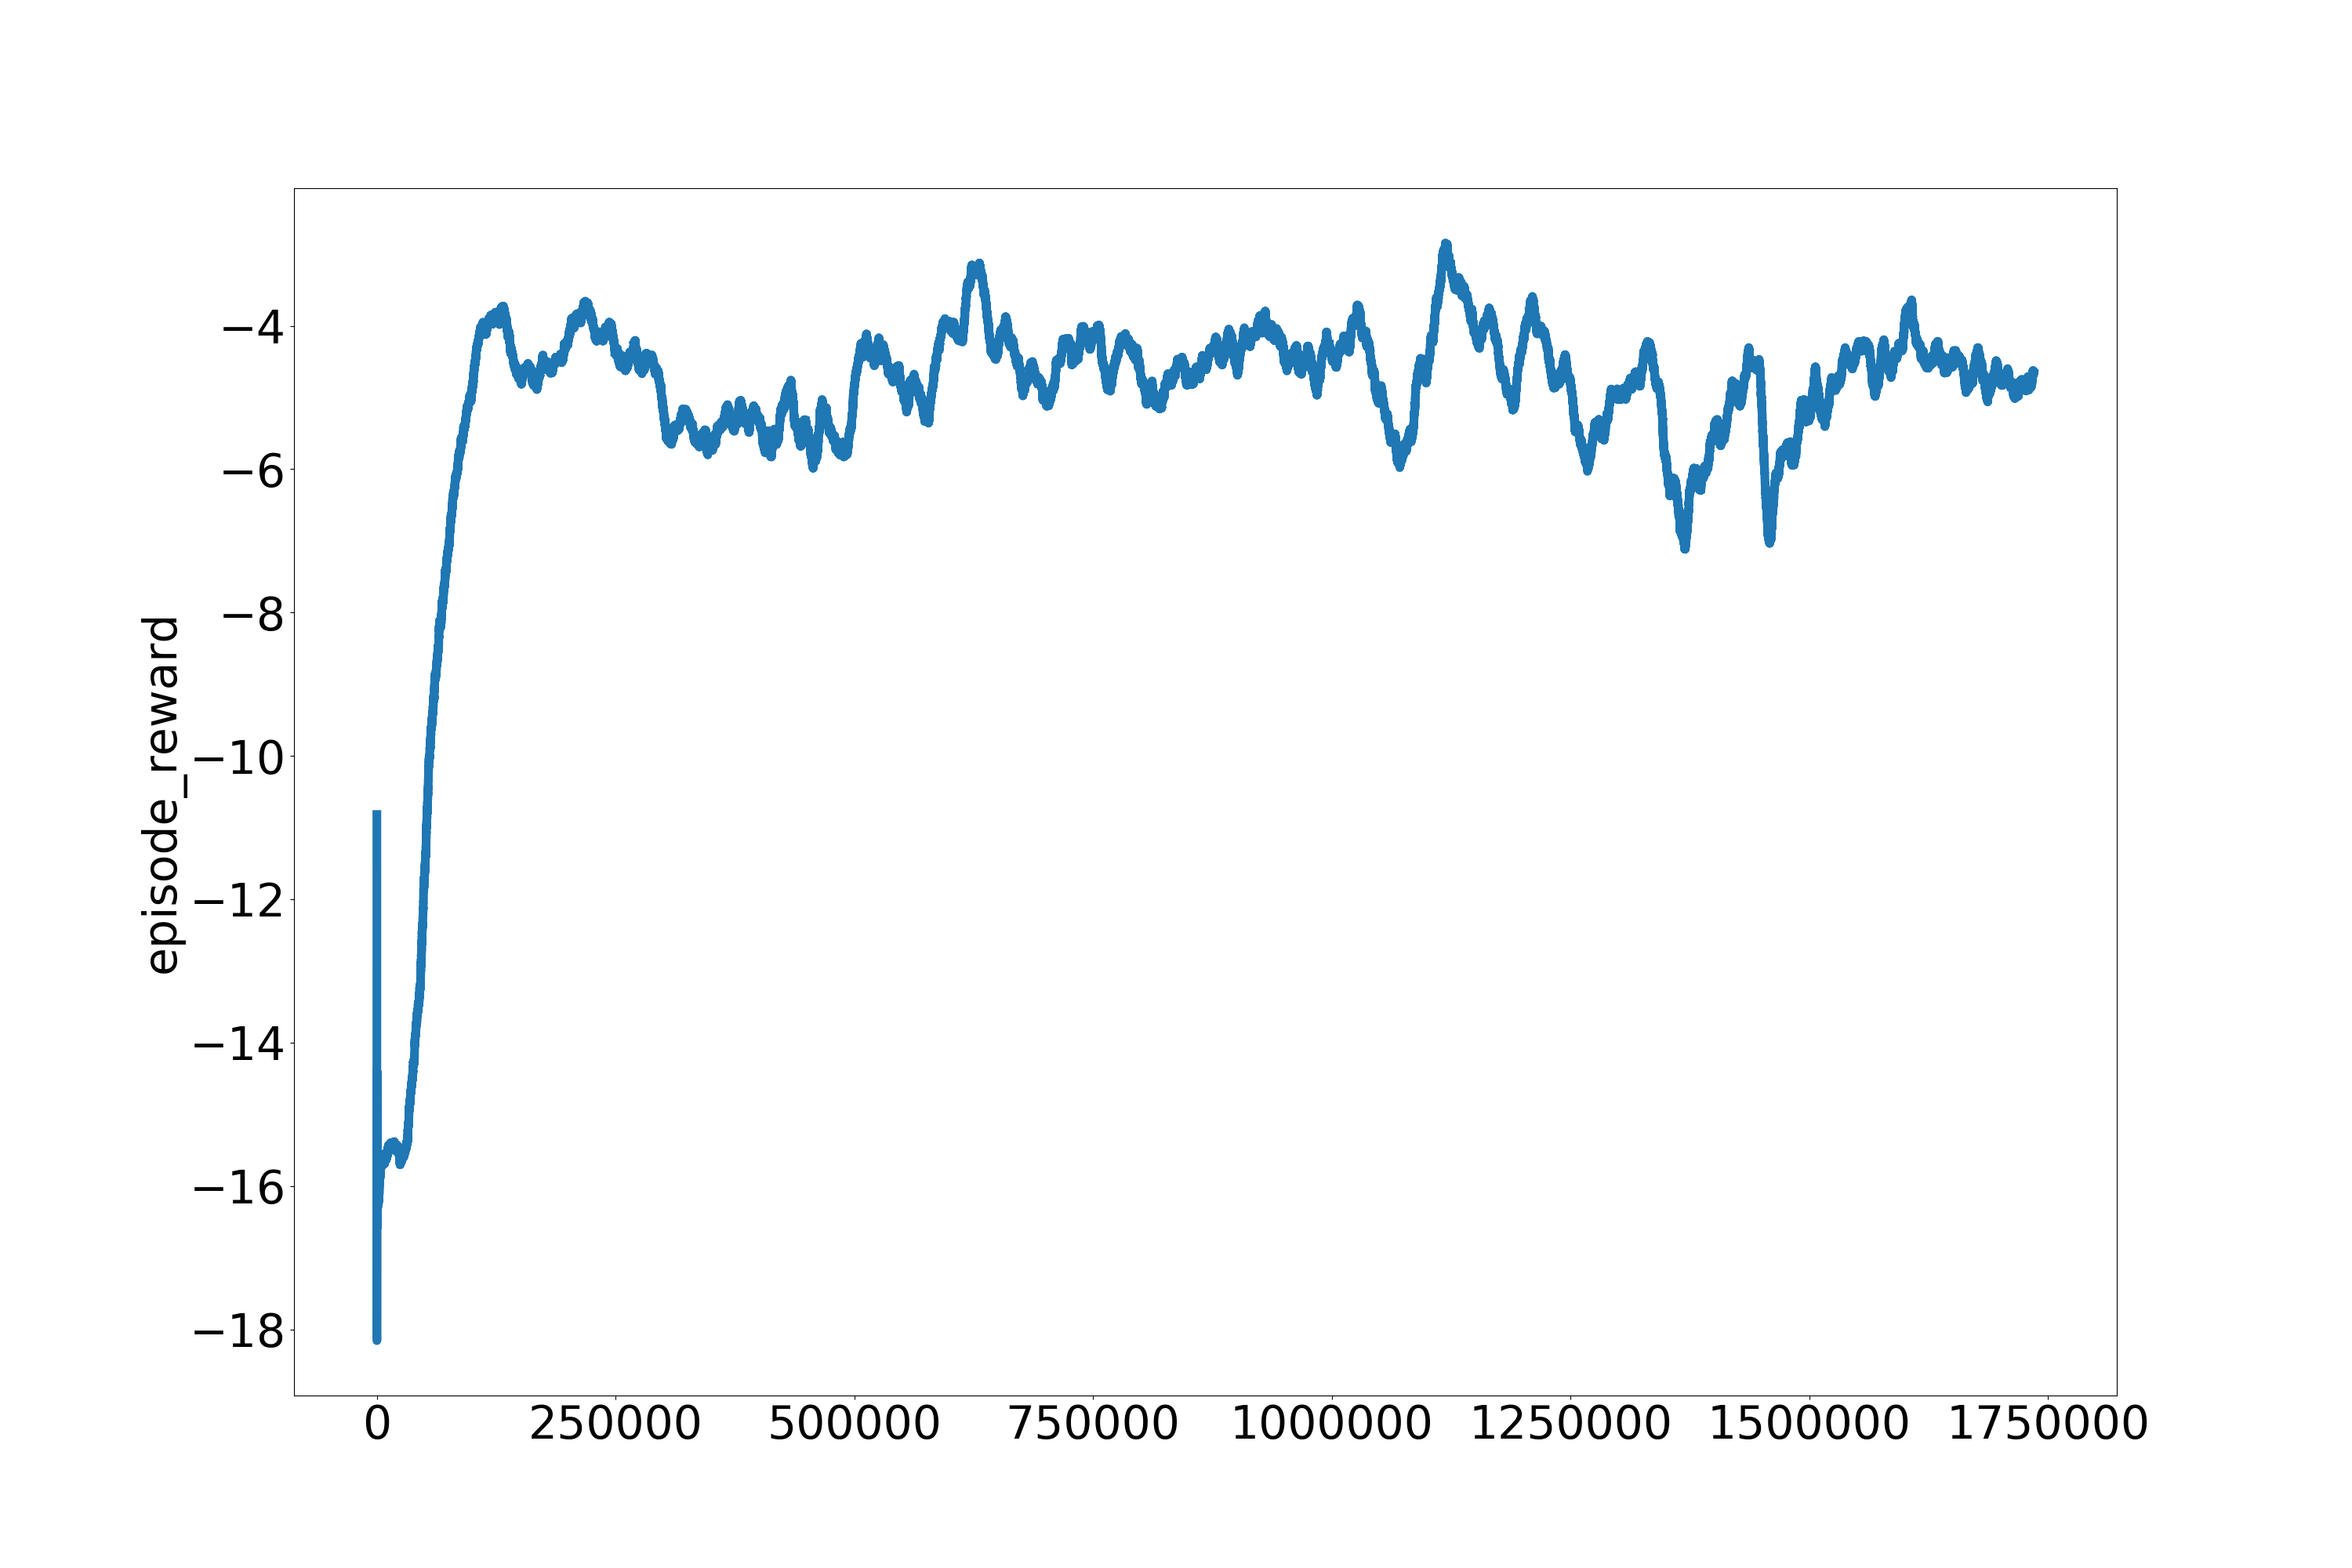
\includegraphics[width=1.1\textwidth]{Pic/First_model/episode_reward.png}
      \caption{Trung bình tích lũy phần thưởng}
      \label{fig:first_model:try_1:avg}
    \end{subfigure}%
    \begin{subfigure}{.5\textwidth}
      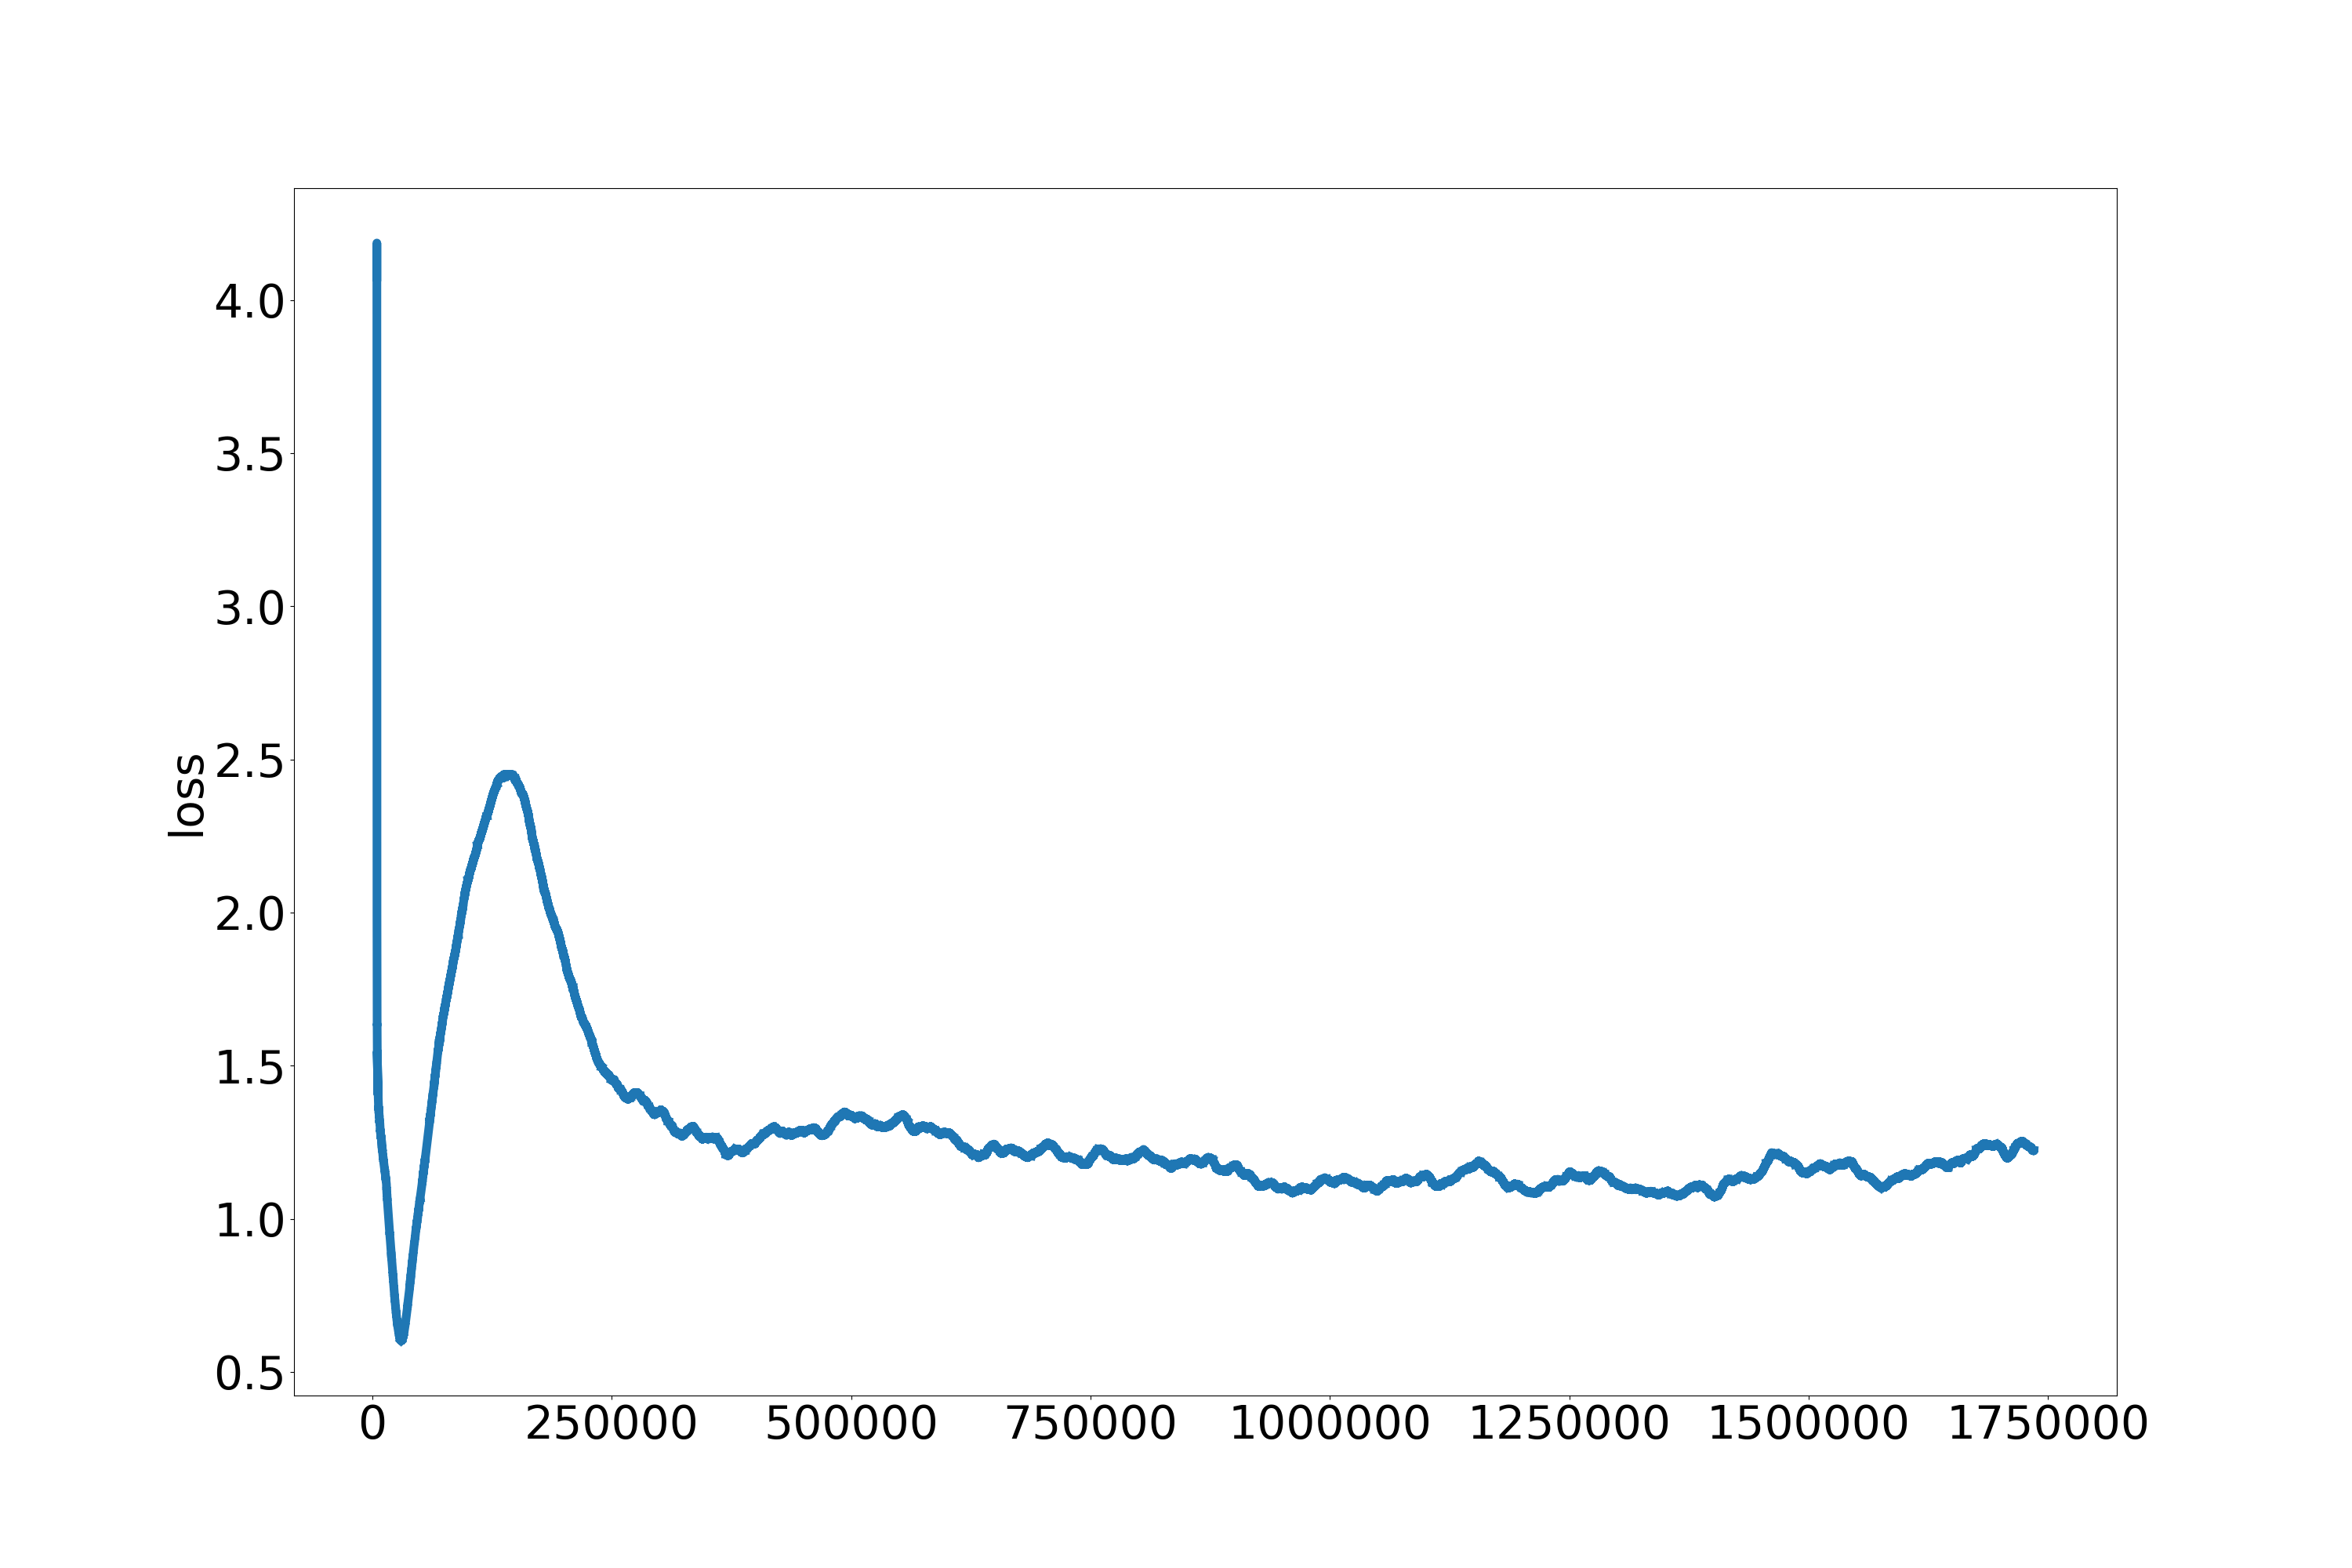
\includegraphics[width=1.1\textwidth]{Pic/First_model/loss.png}
      \caption{Hàm mất mát}
      \label{fig:first_model:try_1:loss}
    \end{subfigure}
    \begin{subfigure}{.5\textwidth}
      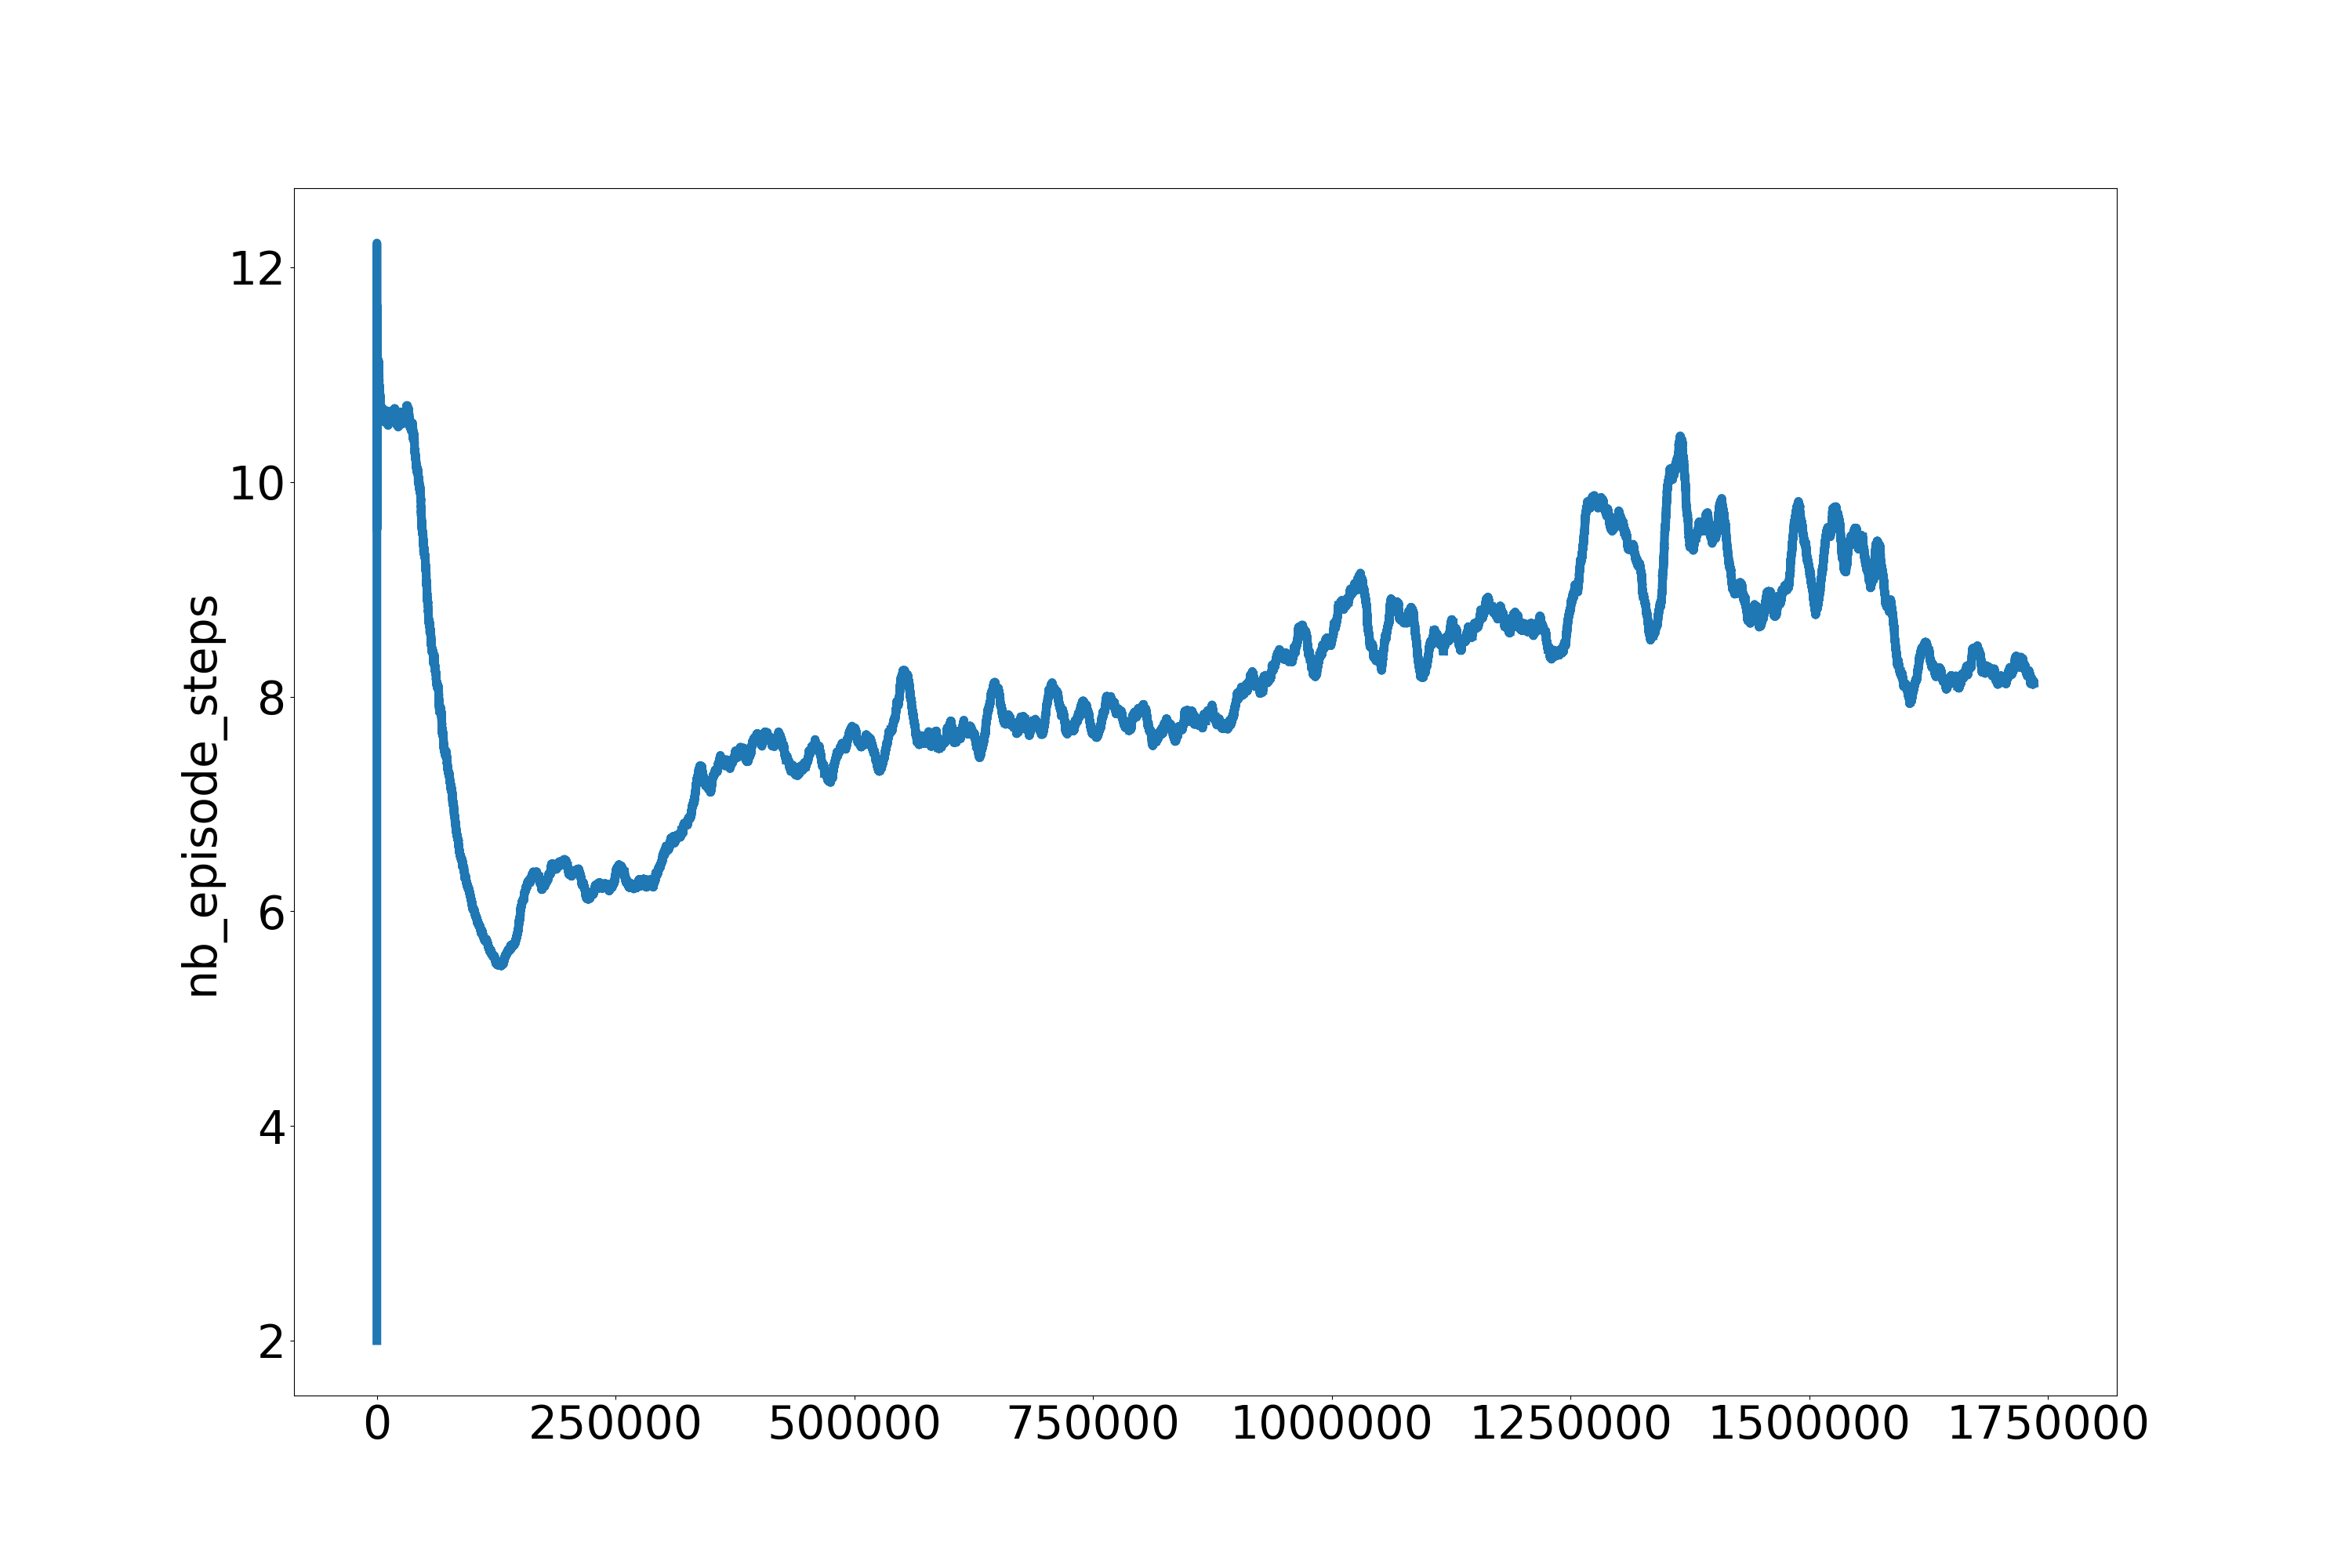
\includegraphics[width=1.1\textwidth]{Pic/First_model/nb_episode_steps.png}
      \caption{Số bước thực hiện}
      \label{fig:first_mode:try_1:step}
    \end{subfigure}%
    \begin{subfigure}{.5\textwidth}
      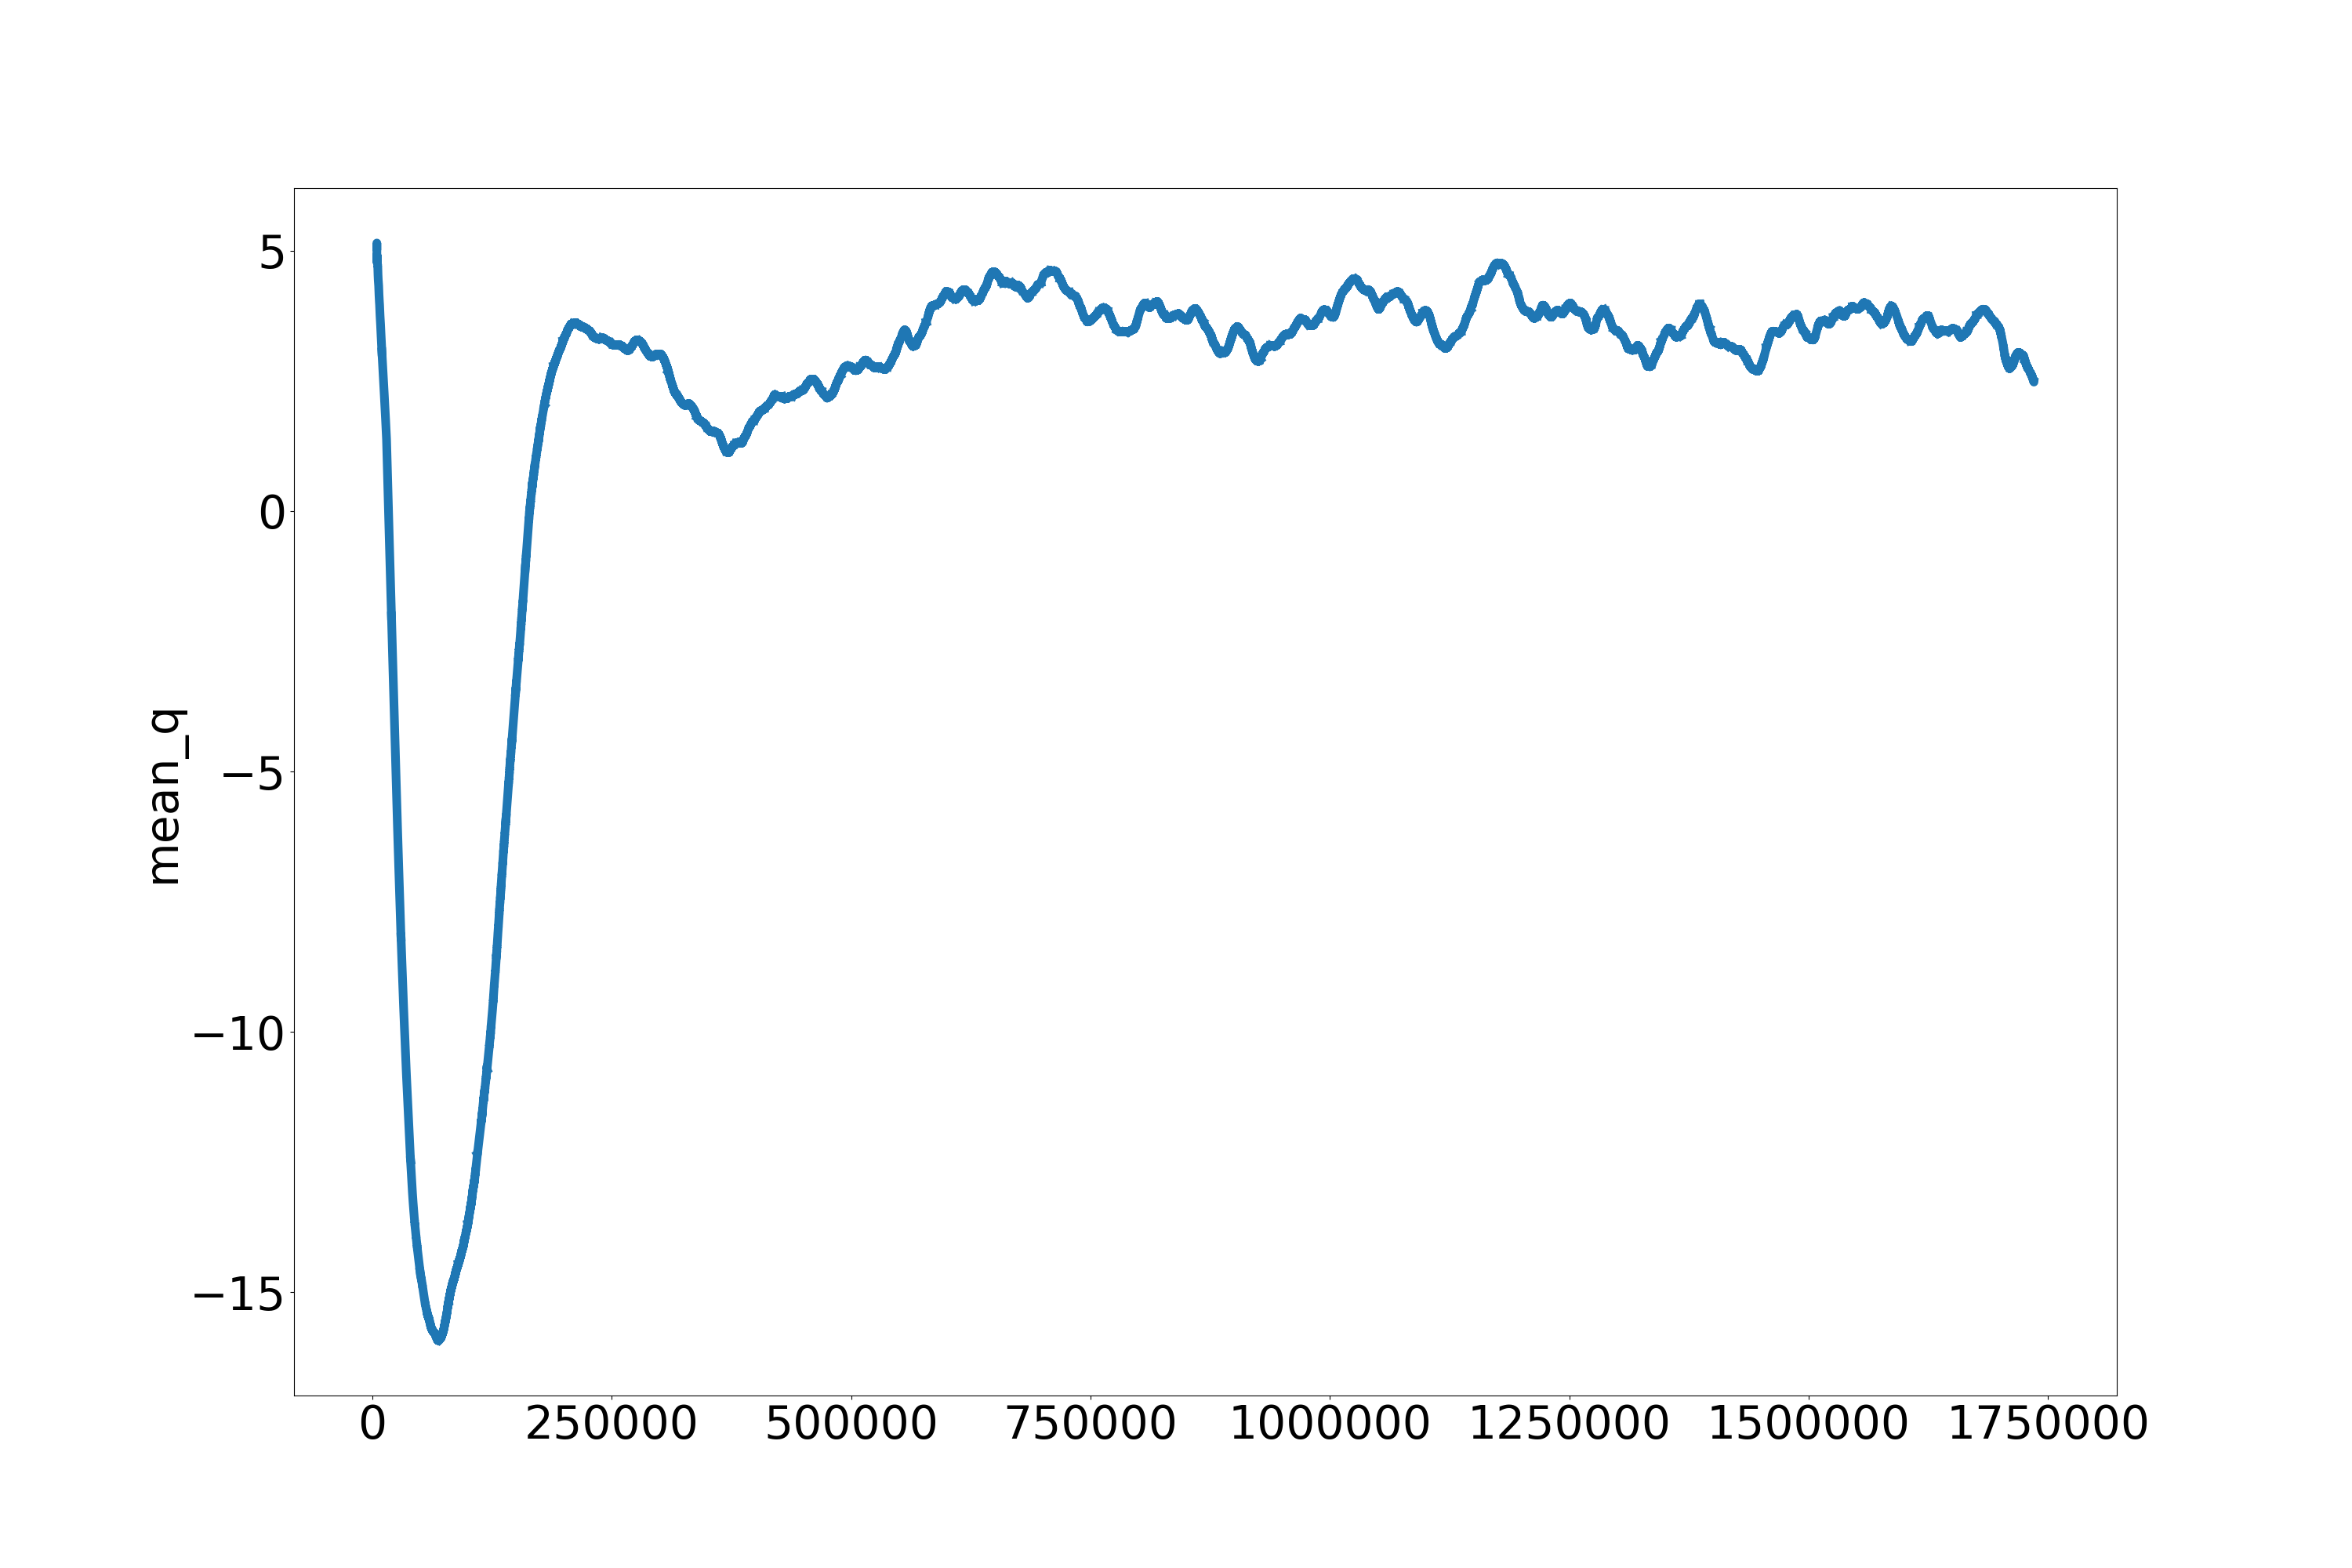
\includegraphics[width=1.1\textwidth]{Pic/First_model/mean_q.png}
      \caption{Trung bình giá trị Q}
      \label{fig:first_model:try1:mean_q}
    \end{subfigure}
\caption[Kết quả của mô hình thứ nhất lần nhất]{\textit{Kết quả của mô hình thứ nhất lần nhất}, một vài các cải thiện được thấy rõ so với mô hình cơ sở trong hình \ref{fig:result_baseline}. Trung bình tích lũy phần thưởng đã ổn định, hàm mất mát hội tụ, số bước thực hiện đã giảm và hàm giá trị Q đã đạt cực đại; Các đánh giá này biểu thị sự biến chuyển tích cực của mô hình thứ nhất đúng với kỳ vọng đặt ra. Tuy nhiên mô hình vẫn chưa tốt, trung bình tích lũy phần thưởng không tăng lên nữa, mà các đồ thị khác đạt "cực đại" nghĩa là rất khó để có thể cải thiện mô hình.}
\label{fig:result_first_model:try_1}
\end{figure}
\vspace{1cm}
\subsubsection{Lần 2}\label{first_model:second_try}
Sau bước chuyển biến tích cực của mô hình \ref{first_model:first_try}, một vài tùy chỉnh về hàm phần thưởng được thực hiện. Ngoài ra để hạn chế việc sử dụng các bước thực hiện, chúng tôi không cho robot thực hiện quá 100 bước mỗi tập. Sự thay đổi về hàm phần thưởng được trình bày sau đây:
\begin{itemize}
    \item Kết quả của \ref{fig:first_model:try_1:avg} phần nhiều các giá trị đều bé hơn không, do đó tác giả muốn tách biệt giữa trường hợp robot thắng nhưng đi rất nhiều ra khỏi đồ thị.
    \begin{subnumcases}{r(s_t,a_t,s_{t+1})=}
        +50 & $s_{t+1}=\text{đích}$ \\
        -50 & $s_{t+1}=\text{chết}$\\
        -\frac{15-\text{vị trí robot}}{(15- 4)\times 10} & \text{còn lại}\label{first_subtract_10}
    \end{subnumcases}
\end{itemize}
So sánh kết quả \ref{fig:result_first_model:try_2} với \ref{fig:result_first_model:try_1} có thể thấy không có sự khác biệt rõ ràng. Tuy nhiên với lần thử hiện tại cho thấy khi giới hạn số bước robot có thể đi thì đồ thị \ref{fig:first_model:try_2:step} không có xu hướng tăng quá nhiều nữa.\\
\begin{figure}[ht]
    \centering
    \begin{subfigure}{.5\textwidth}
      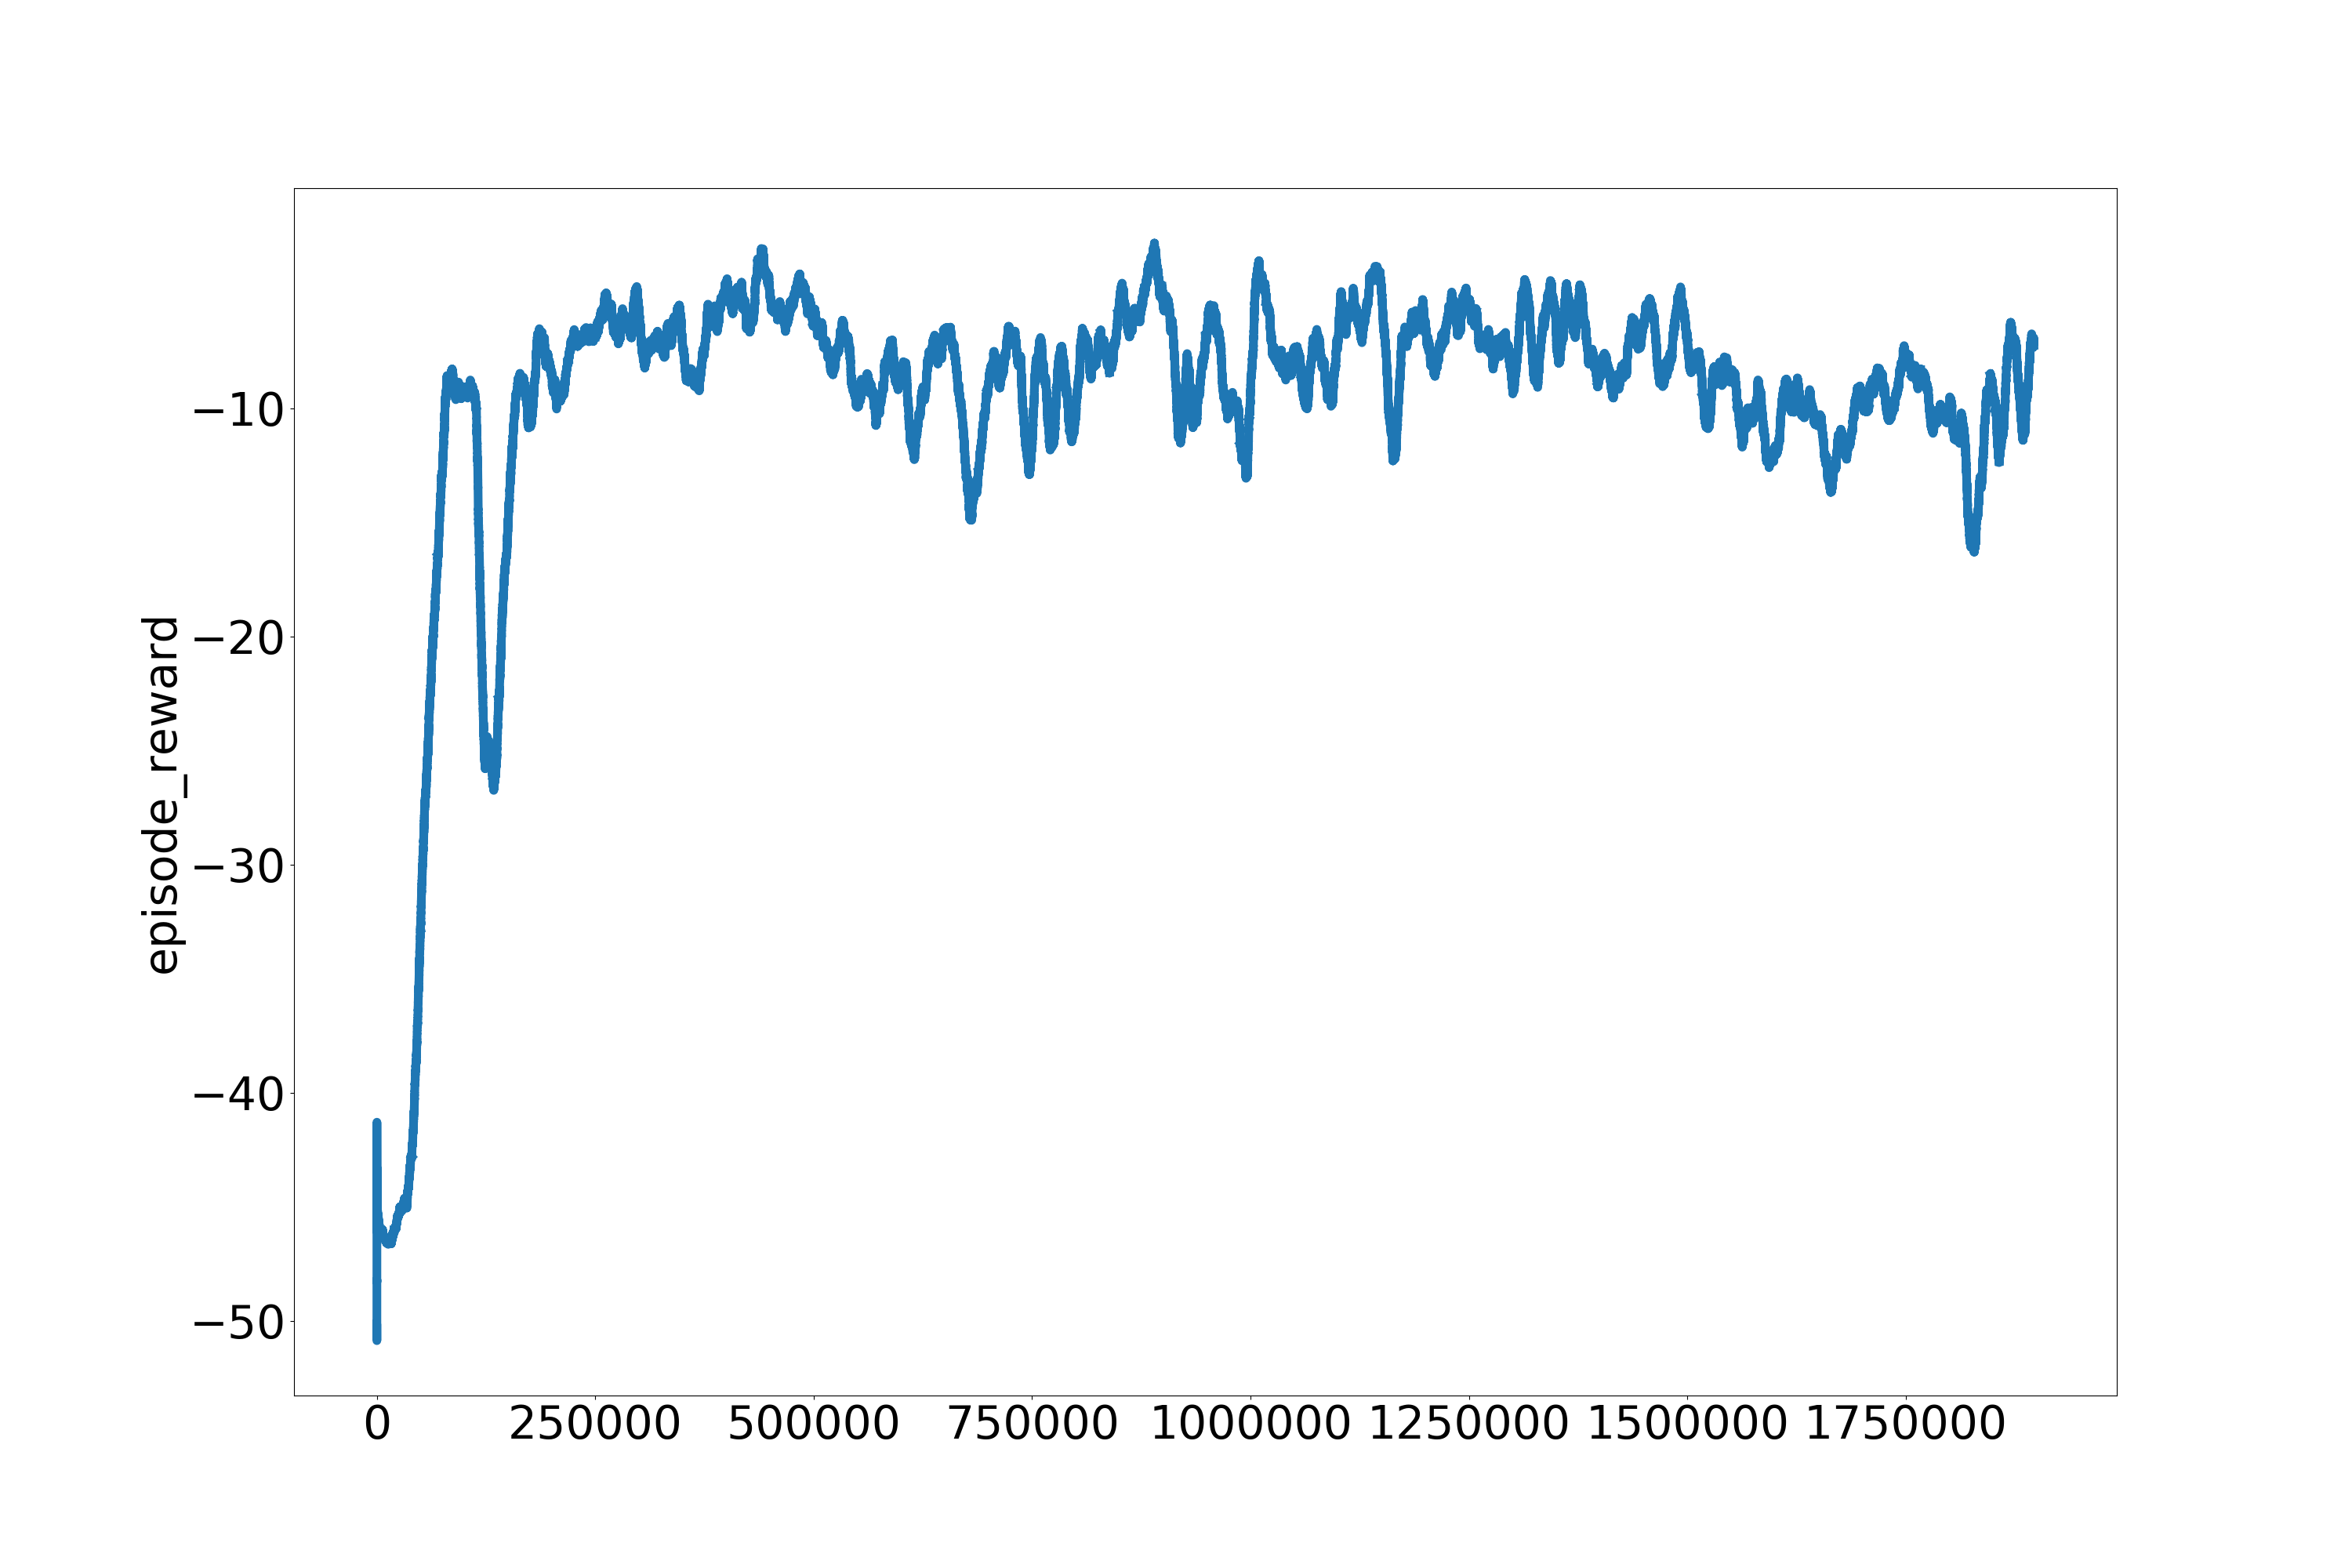
\includegraphics[width=1.1\textwidth]{Pic/First_model_50_reward/episode_reward.png}
      \caption{Trung bình tích lũy phần thưởng}
      \label{fig:first_model:try_2:avg}
    \end{subfigure}%
    \begin{subfigure}{.5\textwidth}
      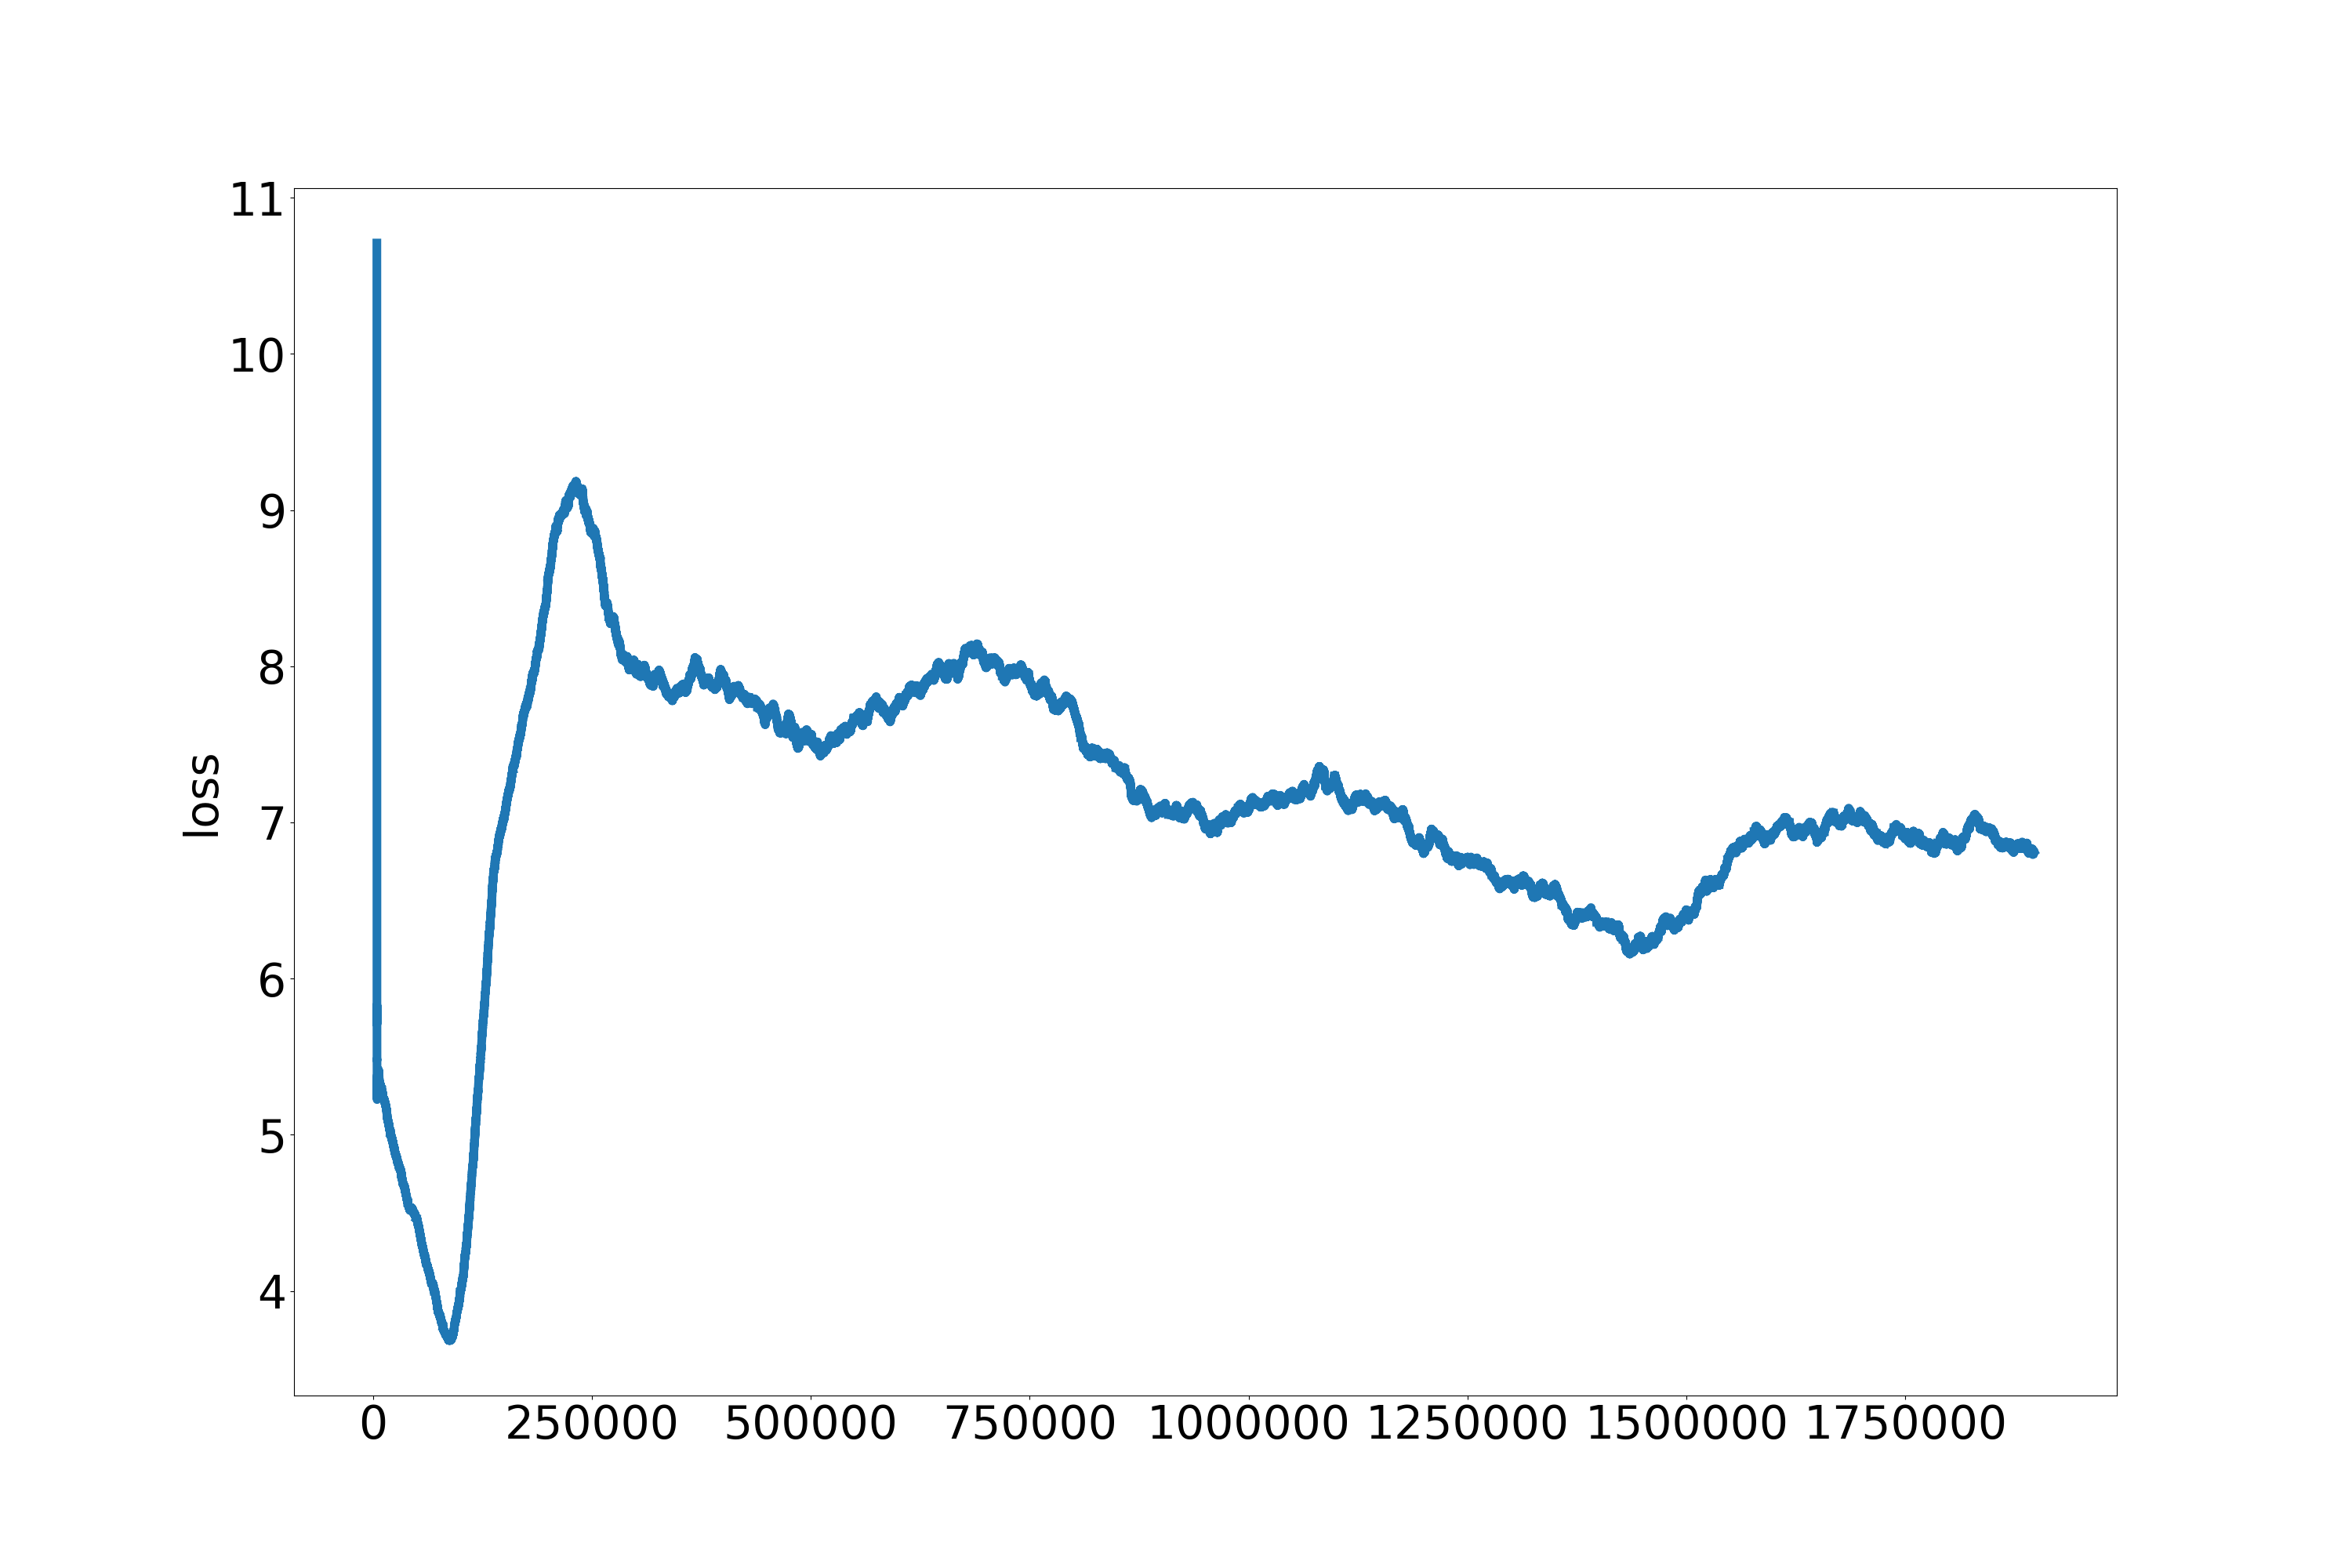
\includegraphics[width=1.1\textwidth]{Pic/First_model_50_reward/loss.png}
      \caption{Hàm mất mát}
      \label{fig:first_model:try_2:loss}
    \end{subfigure}
    \begin{subfigure}{.5\textwidth}
      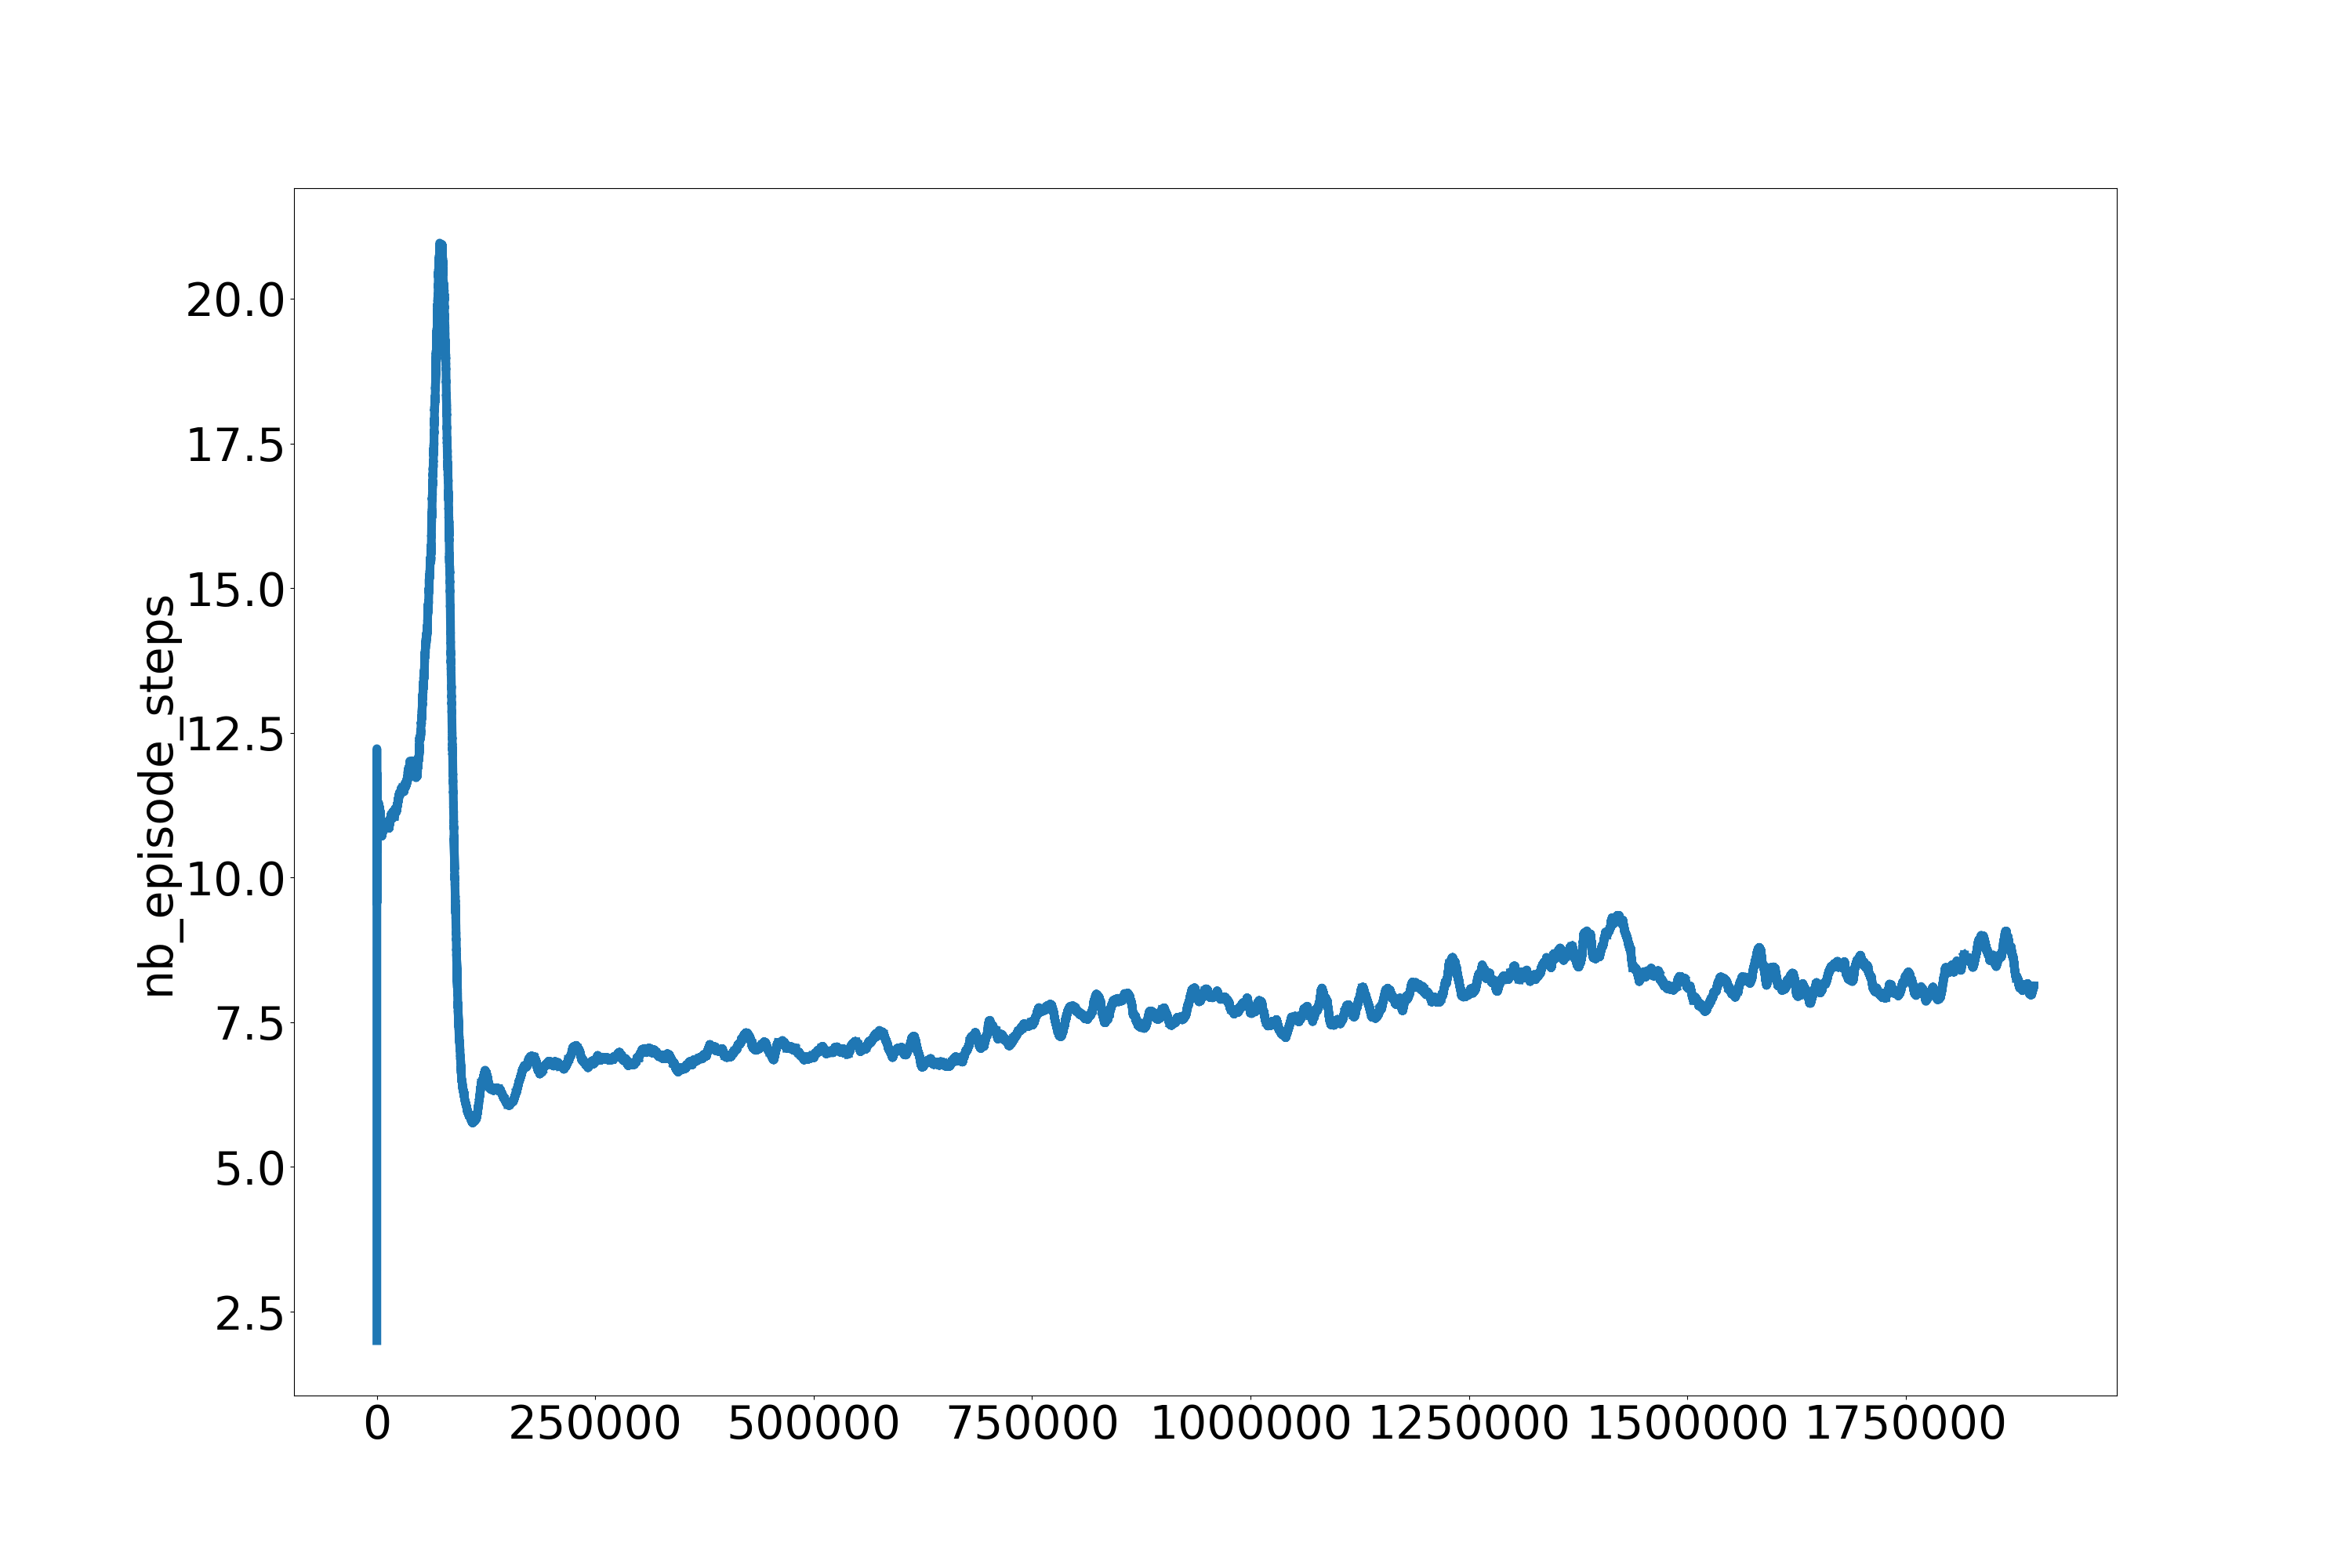
\includegraphics[width=1.1\textwidth]{Pic/First_model_50_reward/nb_episode_steps.png}
      \caption{Số bước thực hiện}
      \label{fig:first_model:try_2:step}
    \end{subfigure}%
    \begin{subfigure}{.5\textwidth}
      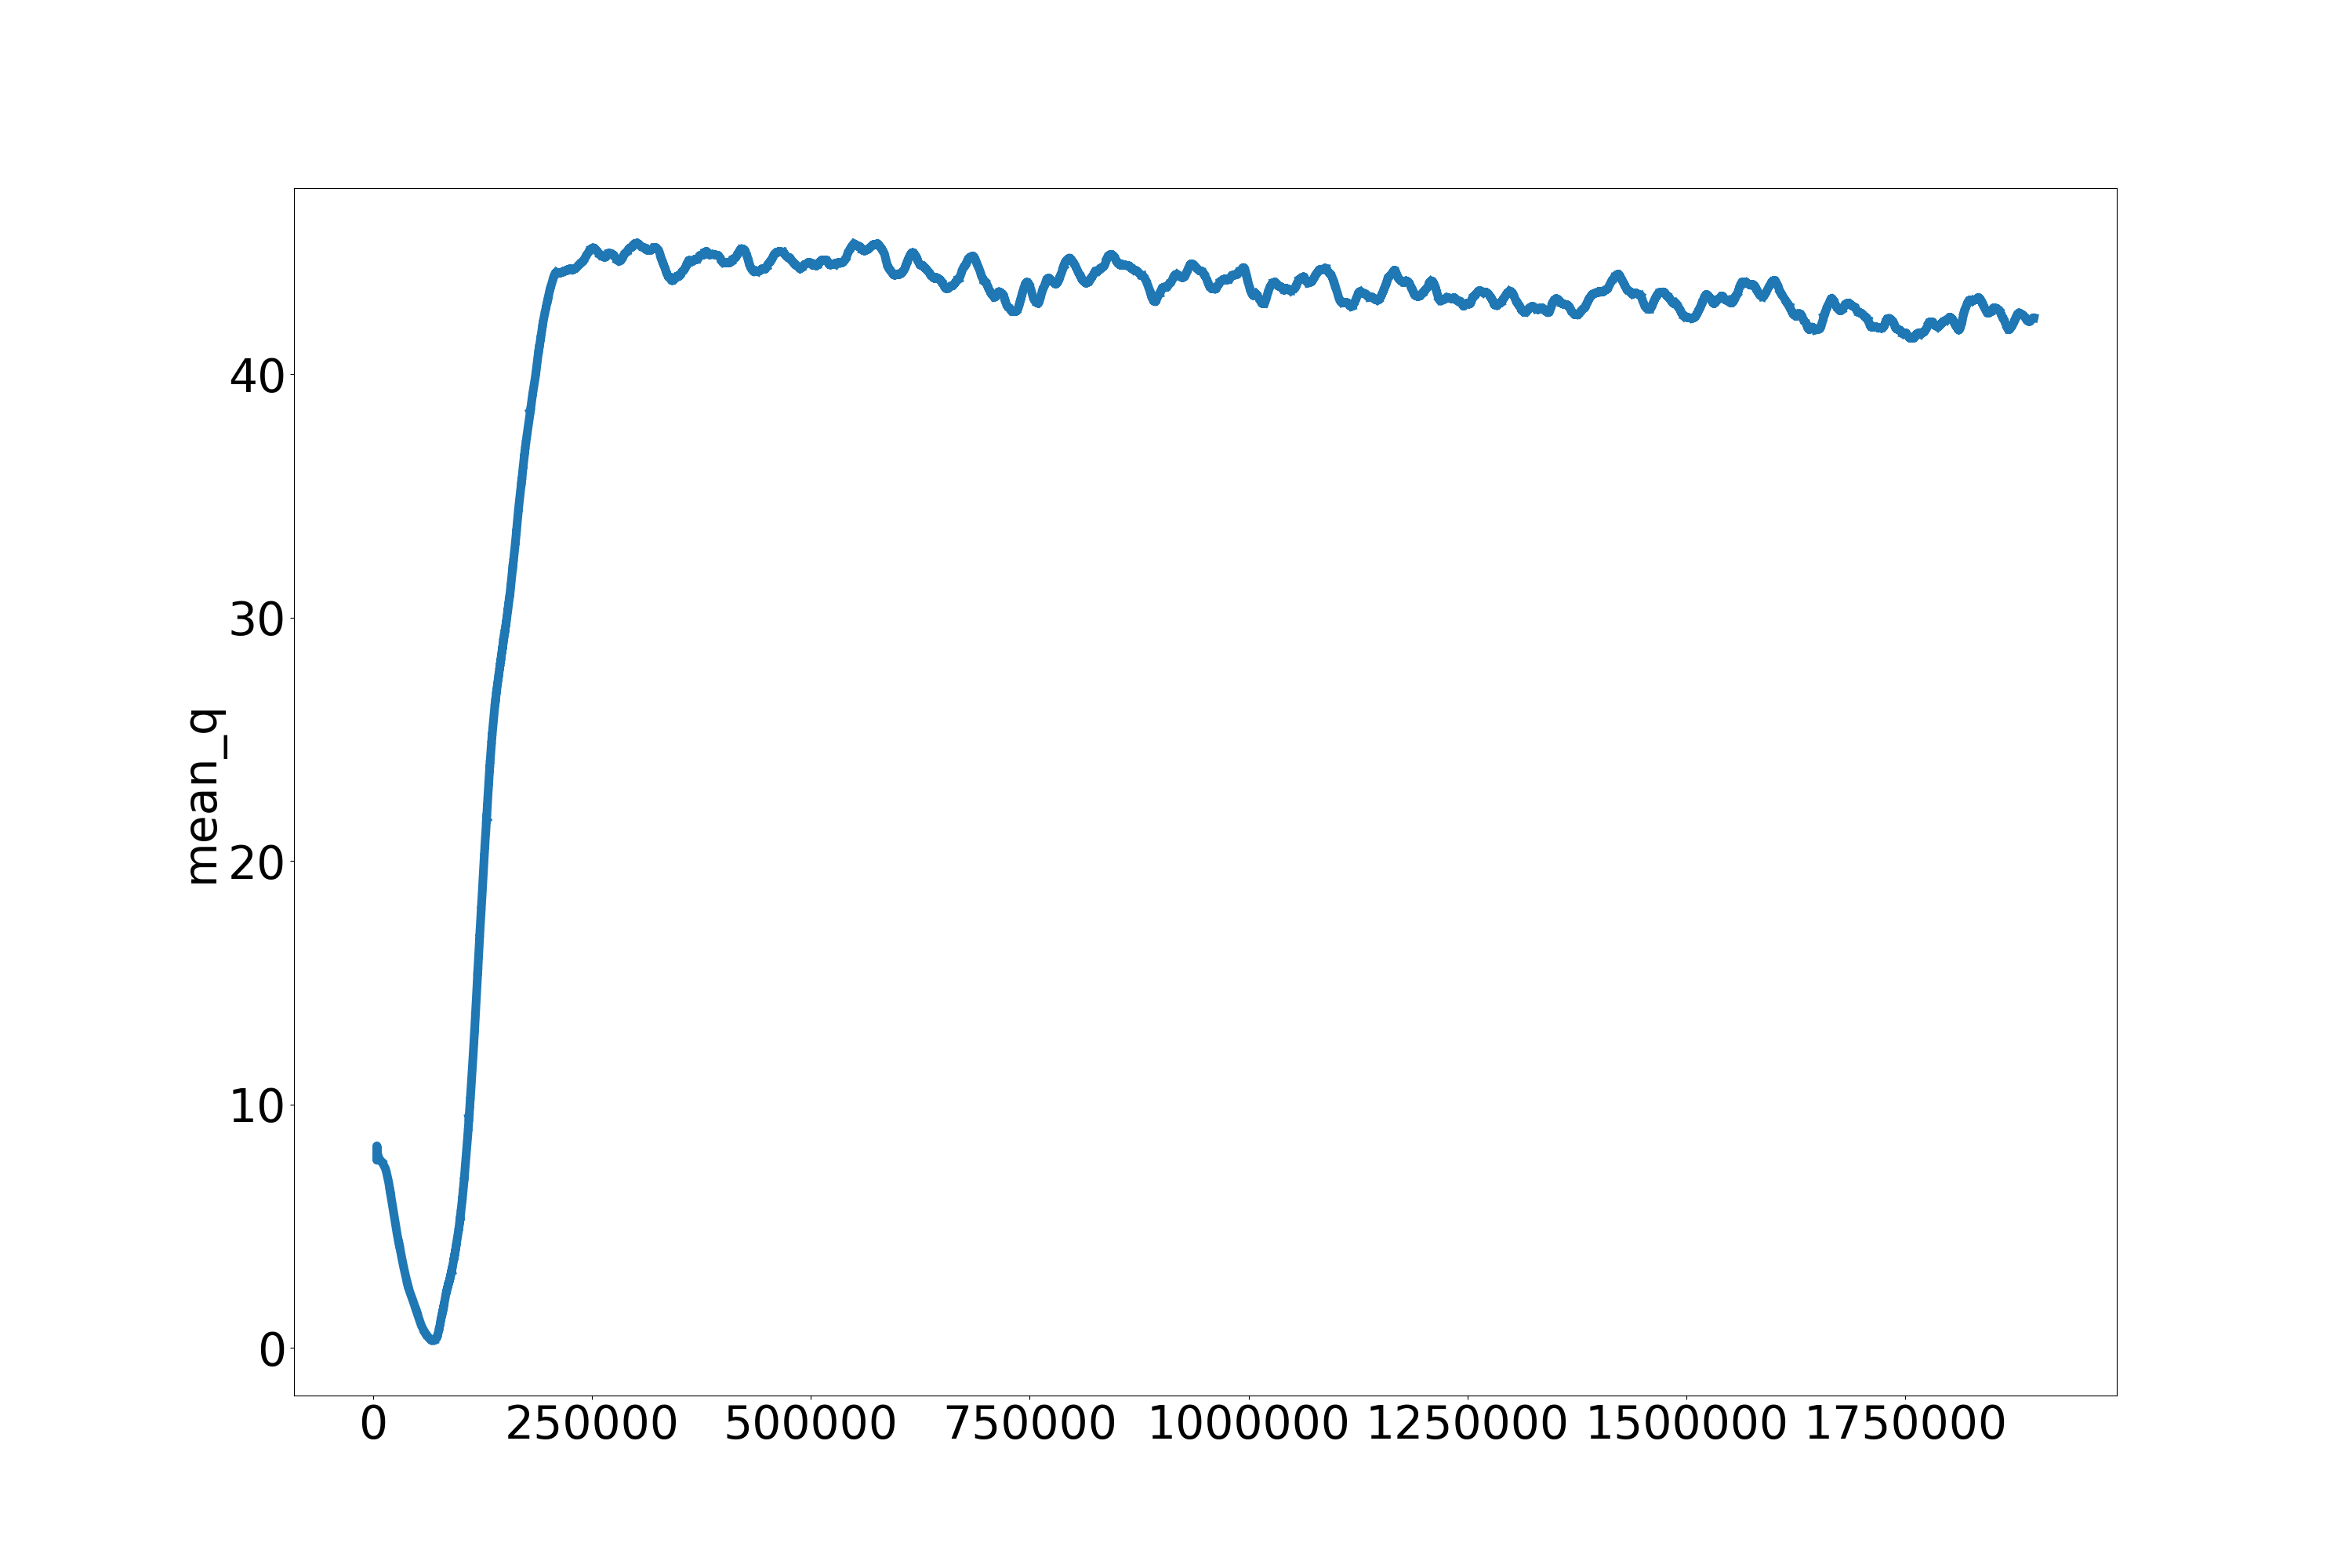
\includegraphics[width=1.1\textwidth]{Pic/First_model_50_reward/mean_q.png}
      \caption{Trung bình giá trị Q}
      \label{fig:first_model:try_2:mean_q}
    \end{subfigure}
\caption[Kết quả của mô hình thứ nhất lần hai]{\textit{Kết quả của mô hình thứ nhất lần hai}, thực nghiệm mô hình thứ hai chứng minh rằng khó có thể đạt được kết quả cao hơn được vì mô hình đã chạm mức "cực đại" của nó.}
\label{fig:result_first_model:try_2}
\end{figure}
\clearpage
\subsection{Mô hình thứ hai}
Dựa vào kết quả của mô hình thứ hai \ref{second_model}, sau hơn 6M bước được thực hiện, so sánh các với thực nghiệm [\ref{fig:result_first_model:try_1}, \ref{fig:result_first_model:try_2}] nhận xét đồ thị khá giống hình dáng nhau. Tuy nhiên khi xét đến trung bình giá trị Q của \ref{fig:result_first_model:try_1} và \ref{fig:resut_second_model}, có thể thấy đồ thị\ref{fig:resut_second_model:mean_q} đã đạt mốc cao hơn trên 7, điều này chứng tỏ mô hình thứ hai đã có cải tiến. Tỷ lệ thắng của mô hình đã chứng tỏ điều này khi đạt \textbf{55.8\%} (lưu ý rằng chỉ mới hơn 6M bước so với 14M bước). Đây là tín hiệu tích cực cho thấy mô hình thứ hai đã có những kết quả tốt hơn và vẫn còn có thể tiếp tục cải thiện khi thực hiện việc huấn luyện thêm nữa.
\begin{figure}[ht]
    \centering
    \begin{subfigure}{.5\textwidth}
      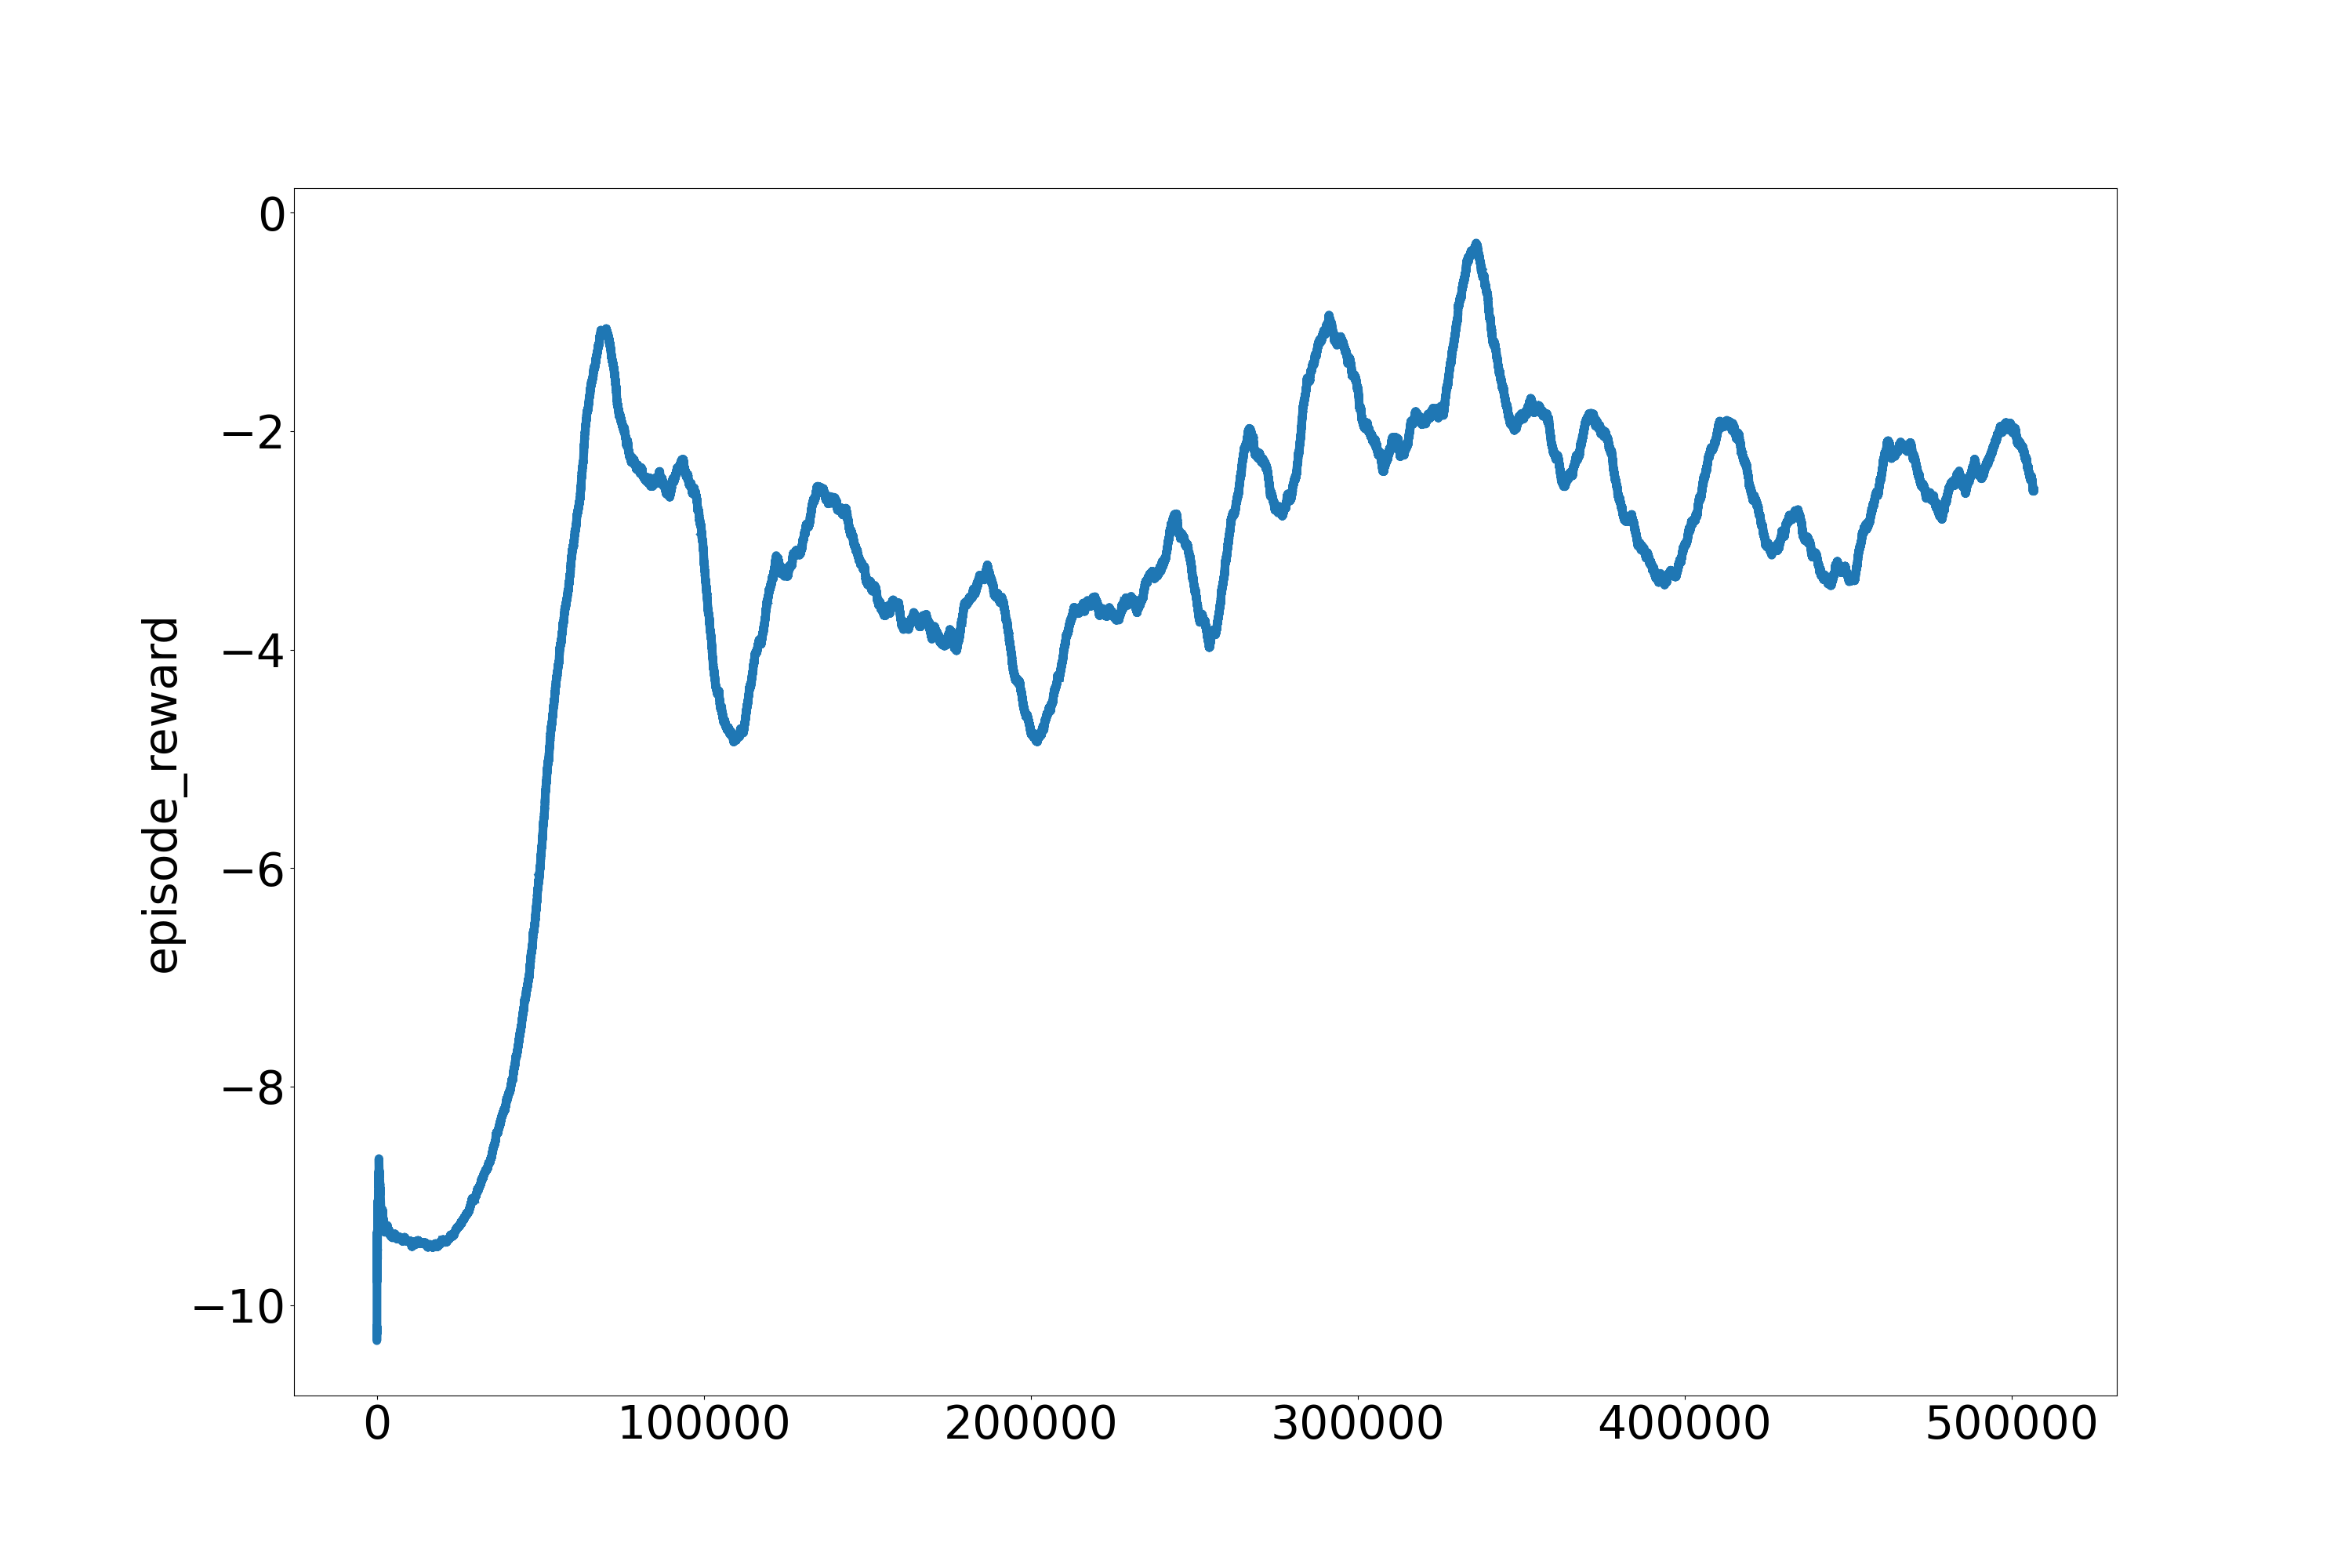
\includegraphics[width=1.1\textwidth]{Pic/Second_model/episode_reward.png}  
      \caption{Trung bình tích lũy phần thưởng}
      \label{fig:resut_second_model:avg}
    \end{subfigure}%
    \begin{subfigure}{.5\textwidth}
      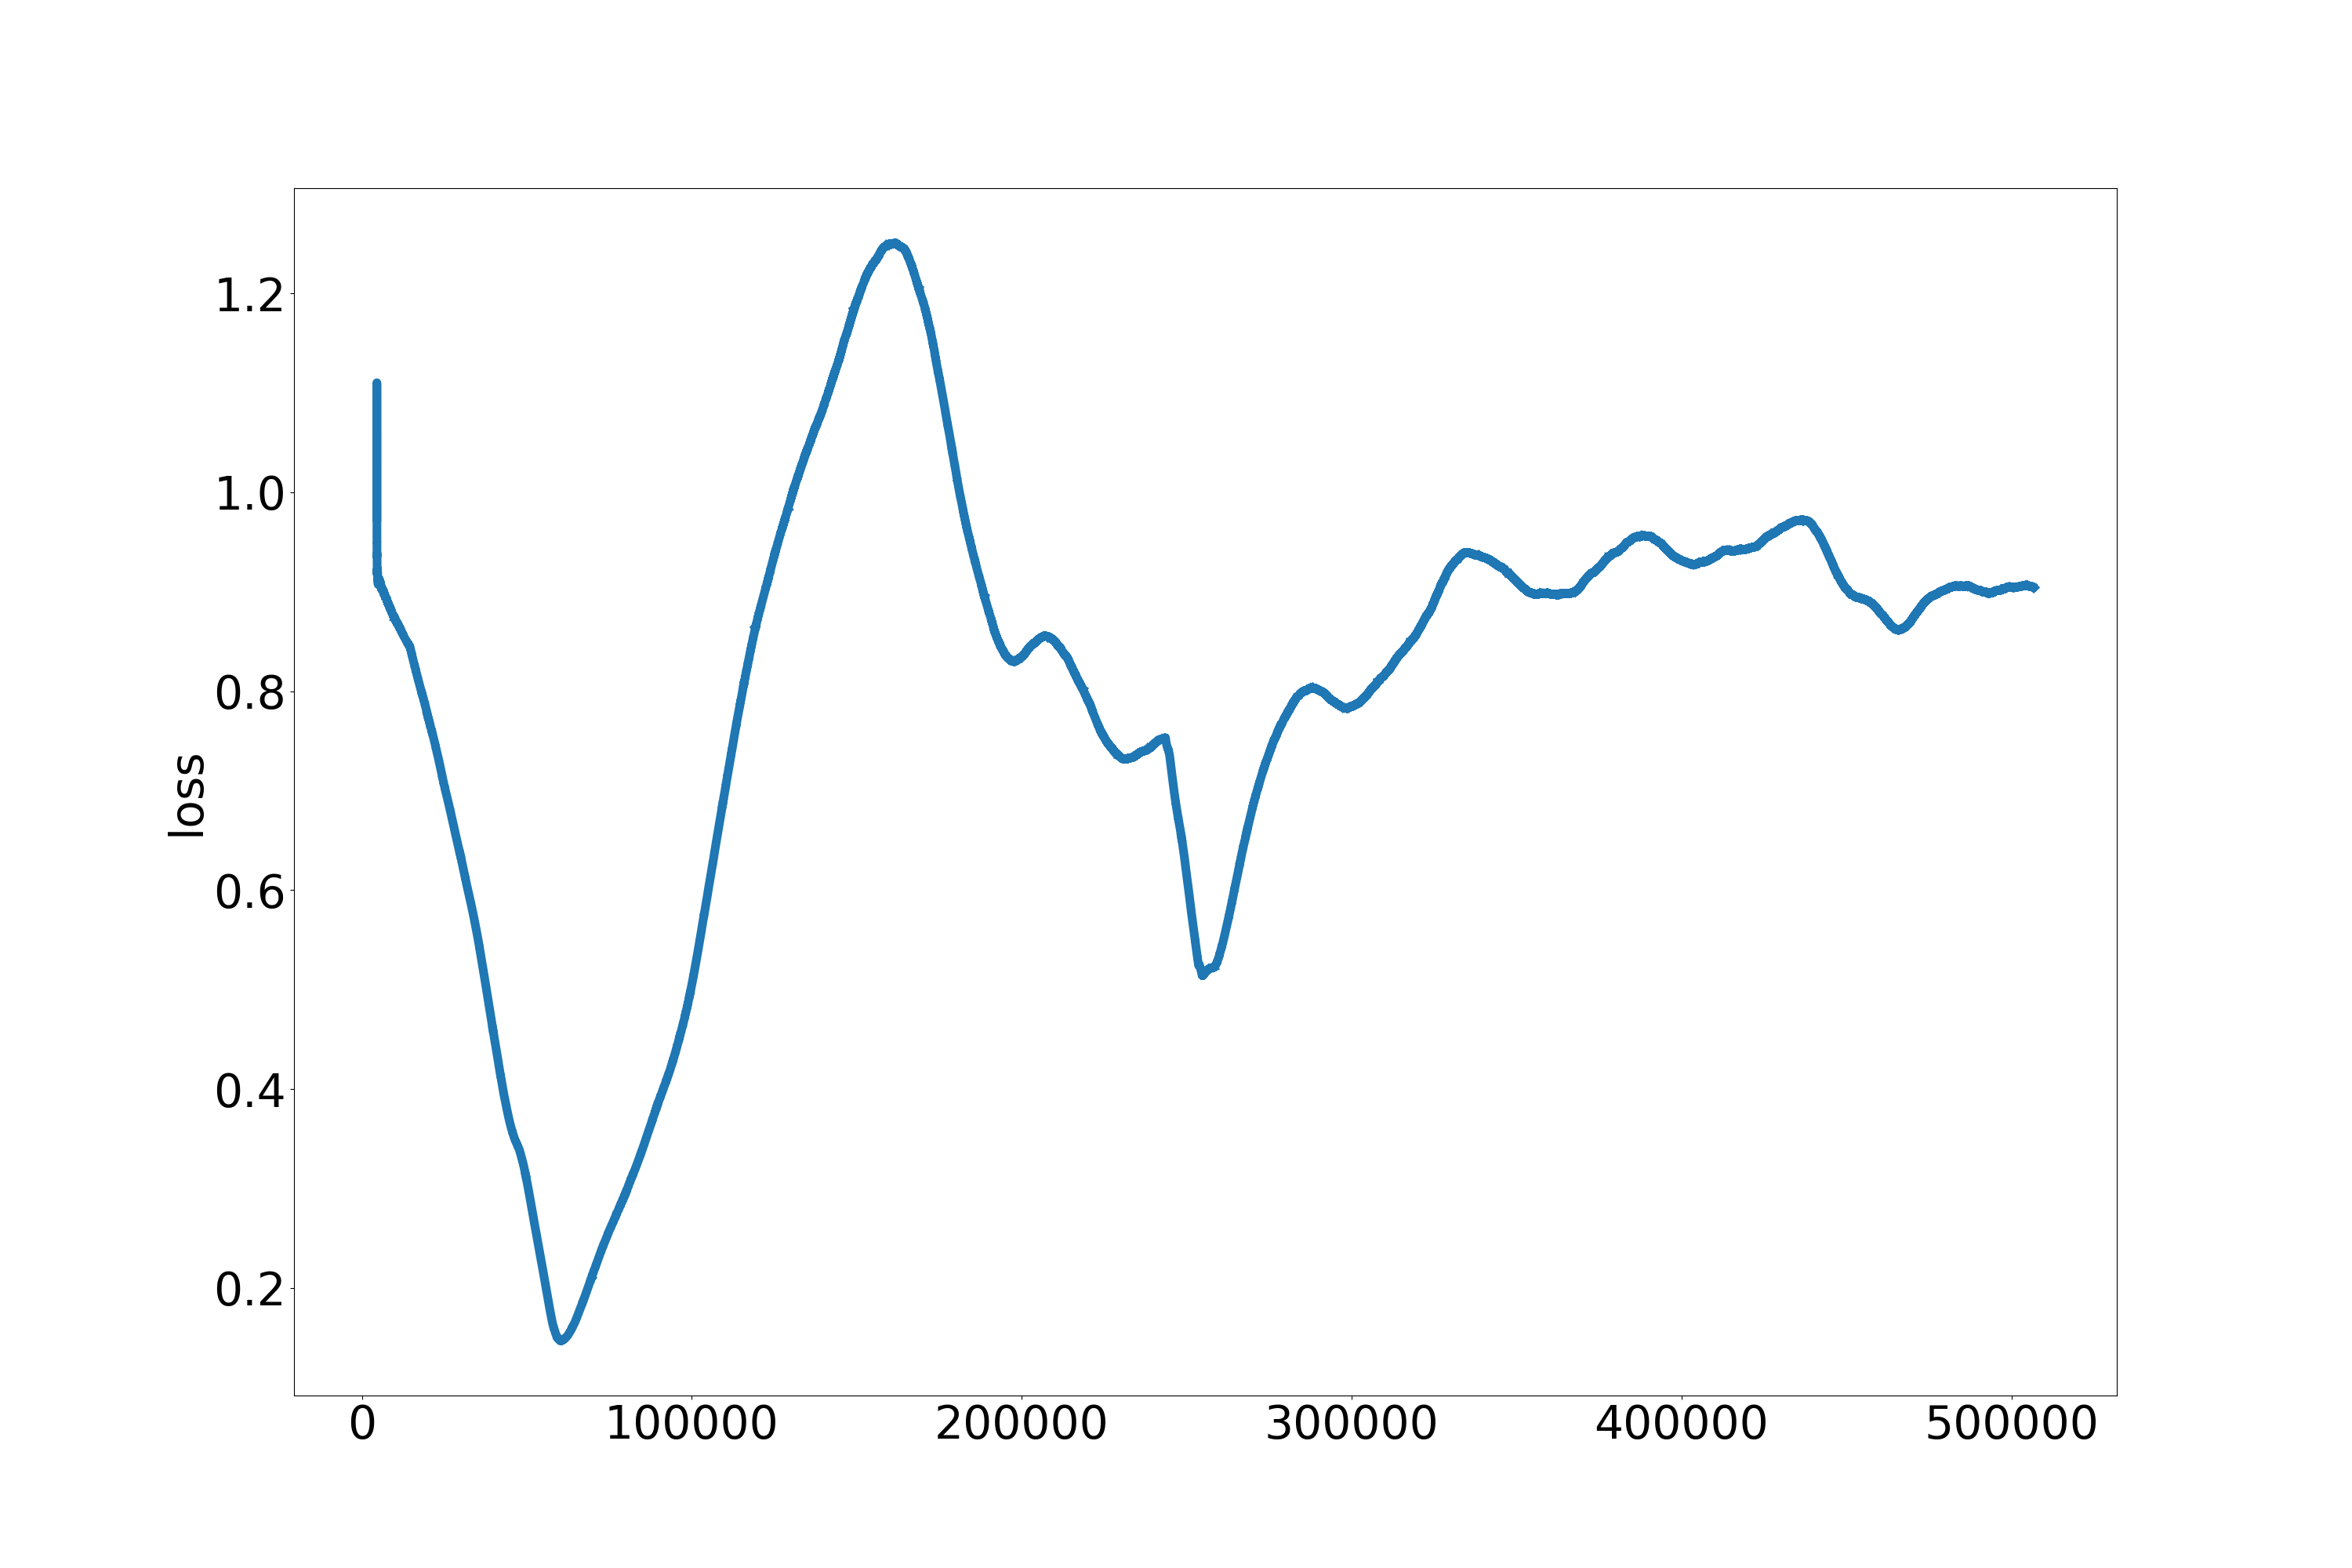
\includegraphics[width=1.1\textwidth]{Pic/Second_model/loss.png}  
      \caption{Hàm mất mát}
      \label{fig:resut_second_model:loss}
    \end{subfigure}\\
    \vspace{1cm}
    \begin{subfigure}{.5\textwidth}
      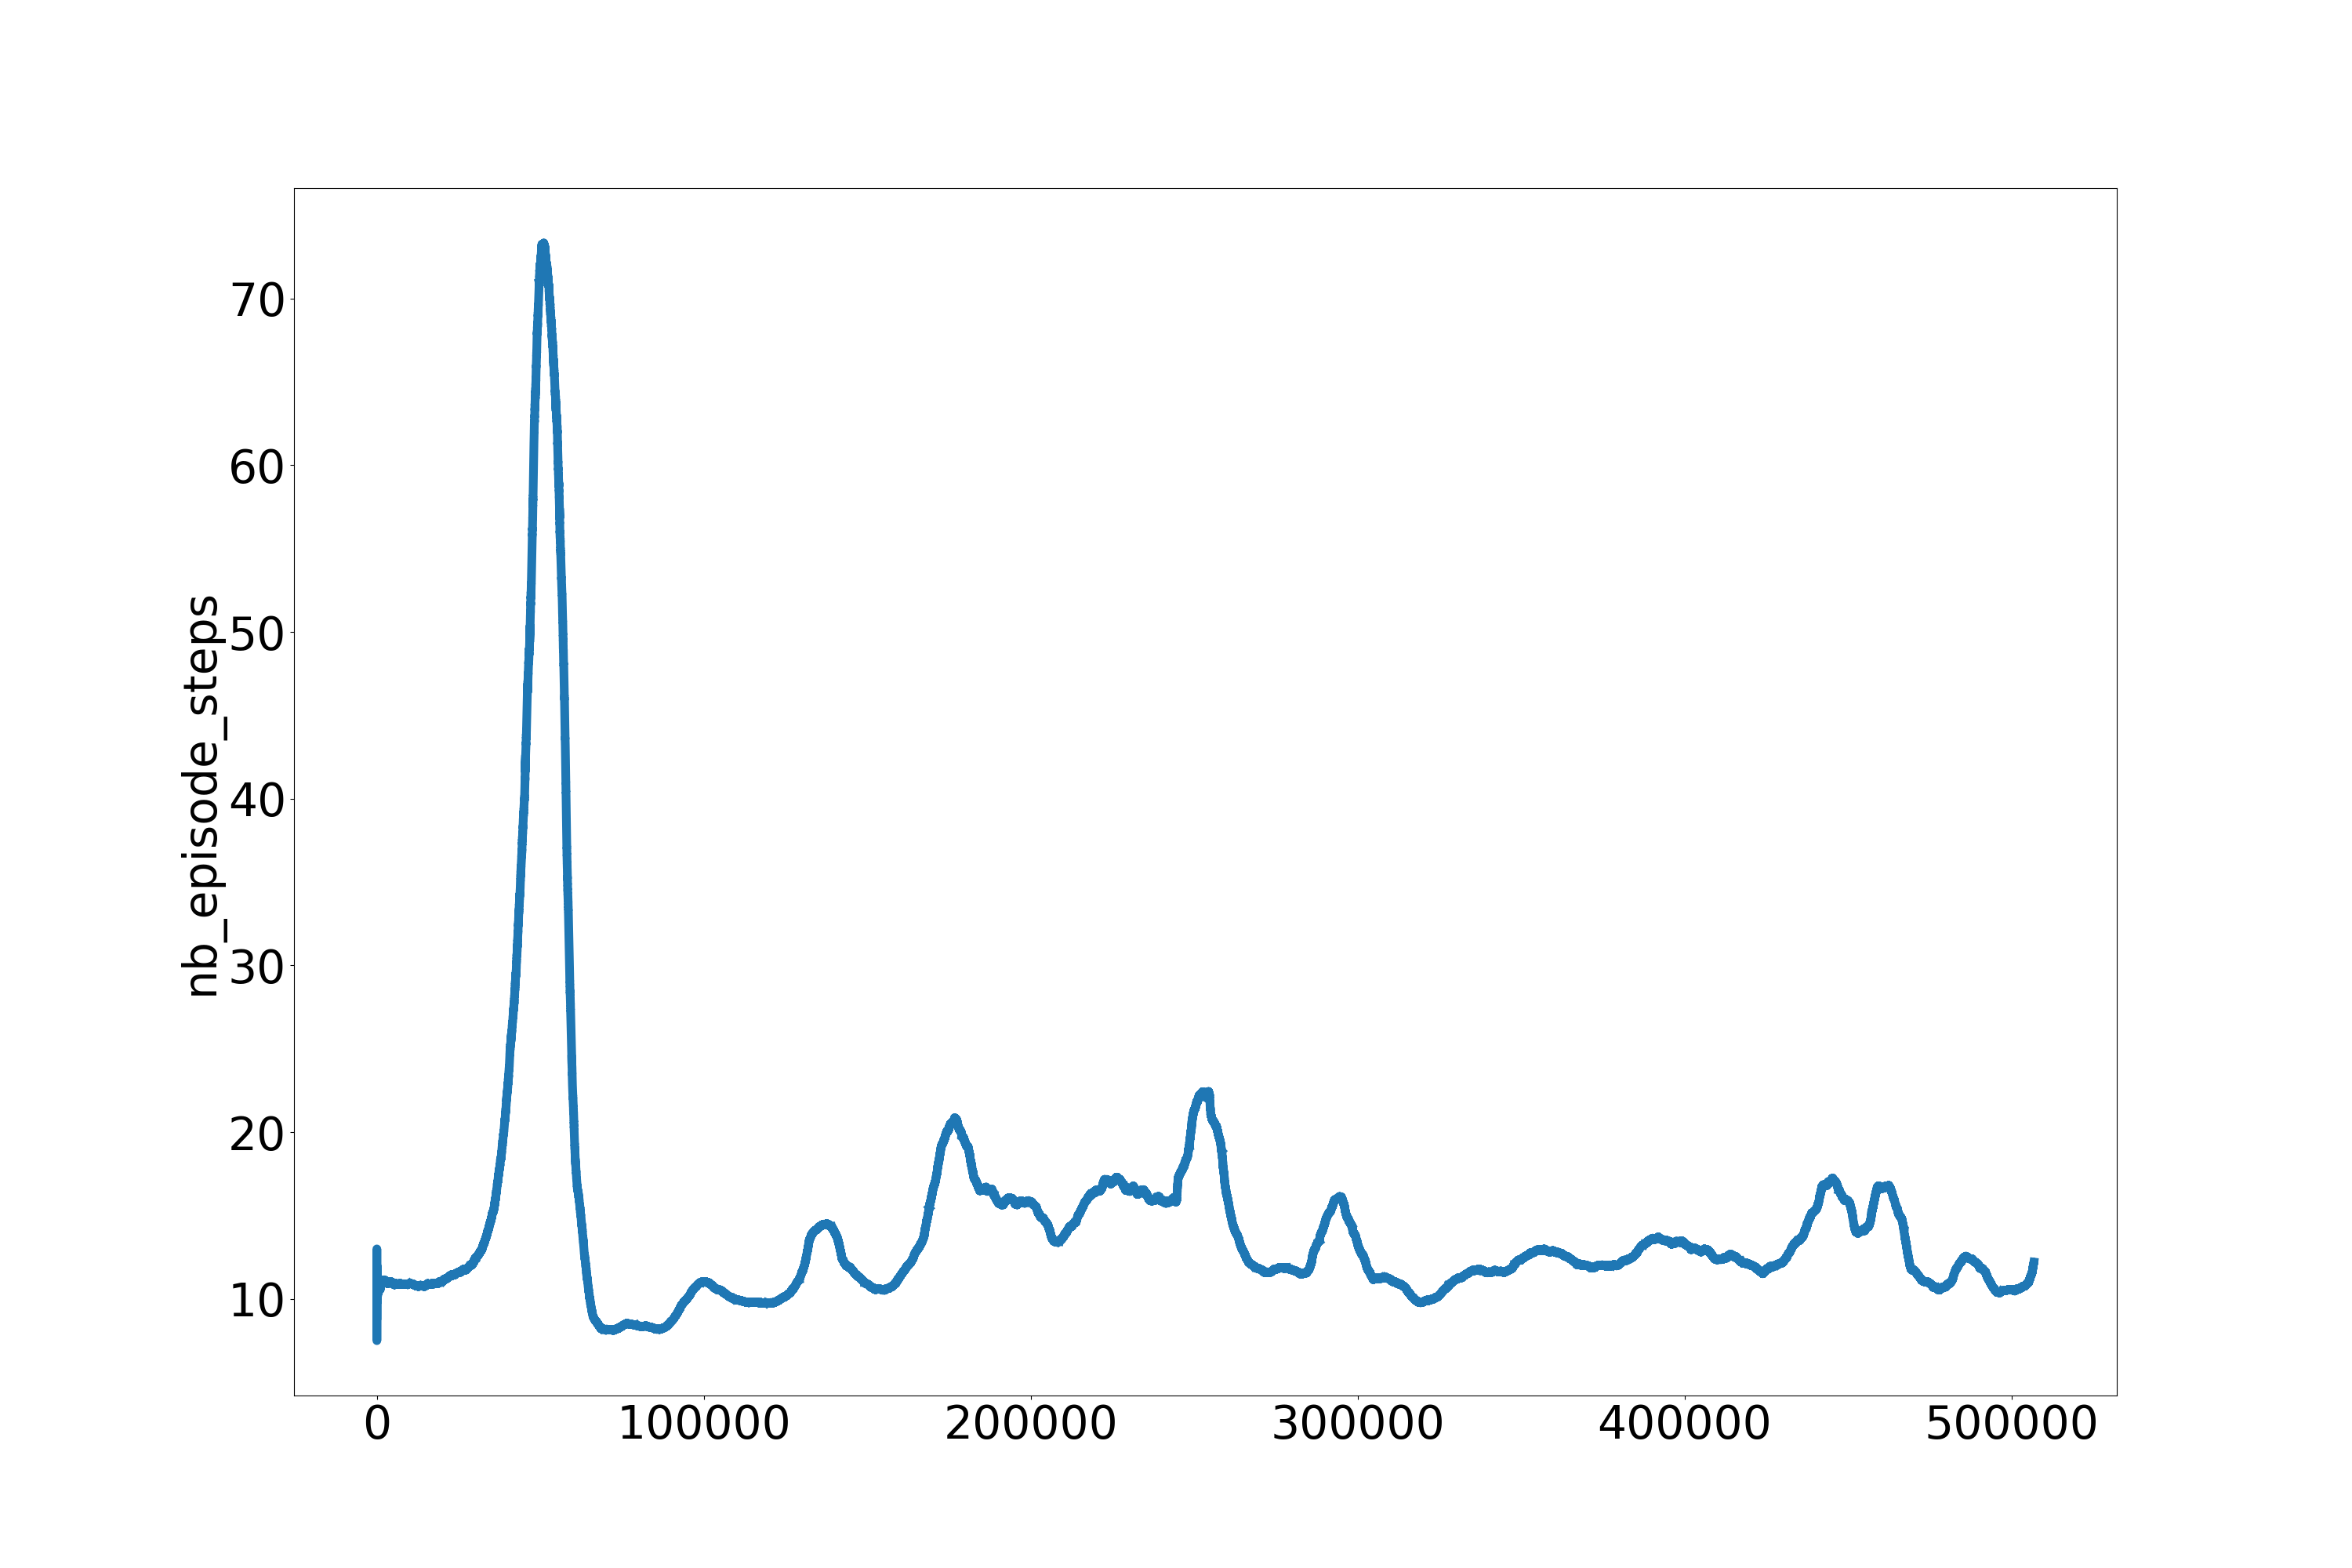
\includegraphics[width=1.1\textwidth]{Pic/Second_model/nb_episode_steps.png}
      \caption{Số bước thực hiện}
      \label{fig:resut_second_model:step}
    \end{subfigure}%
    \begin{subfigure}{.5\textwidth}
      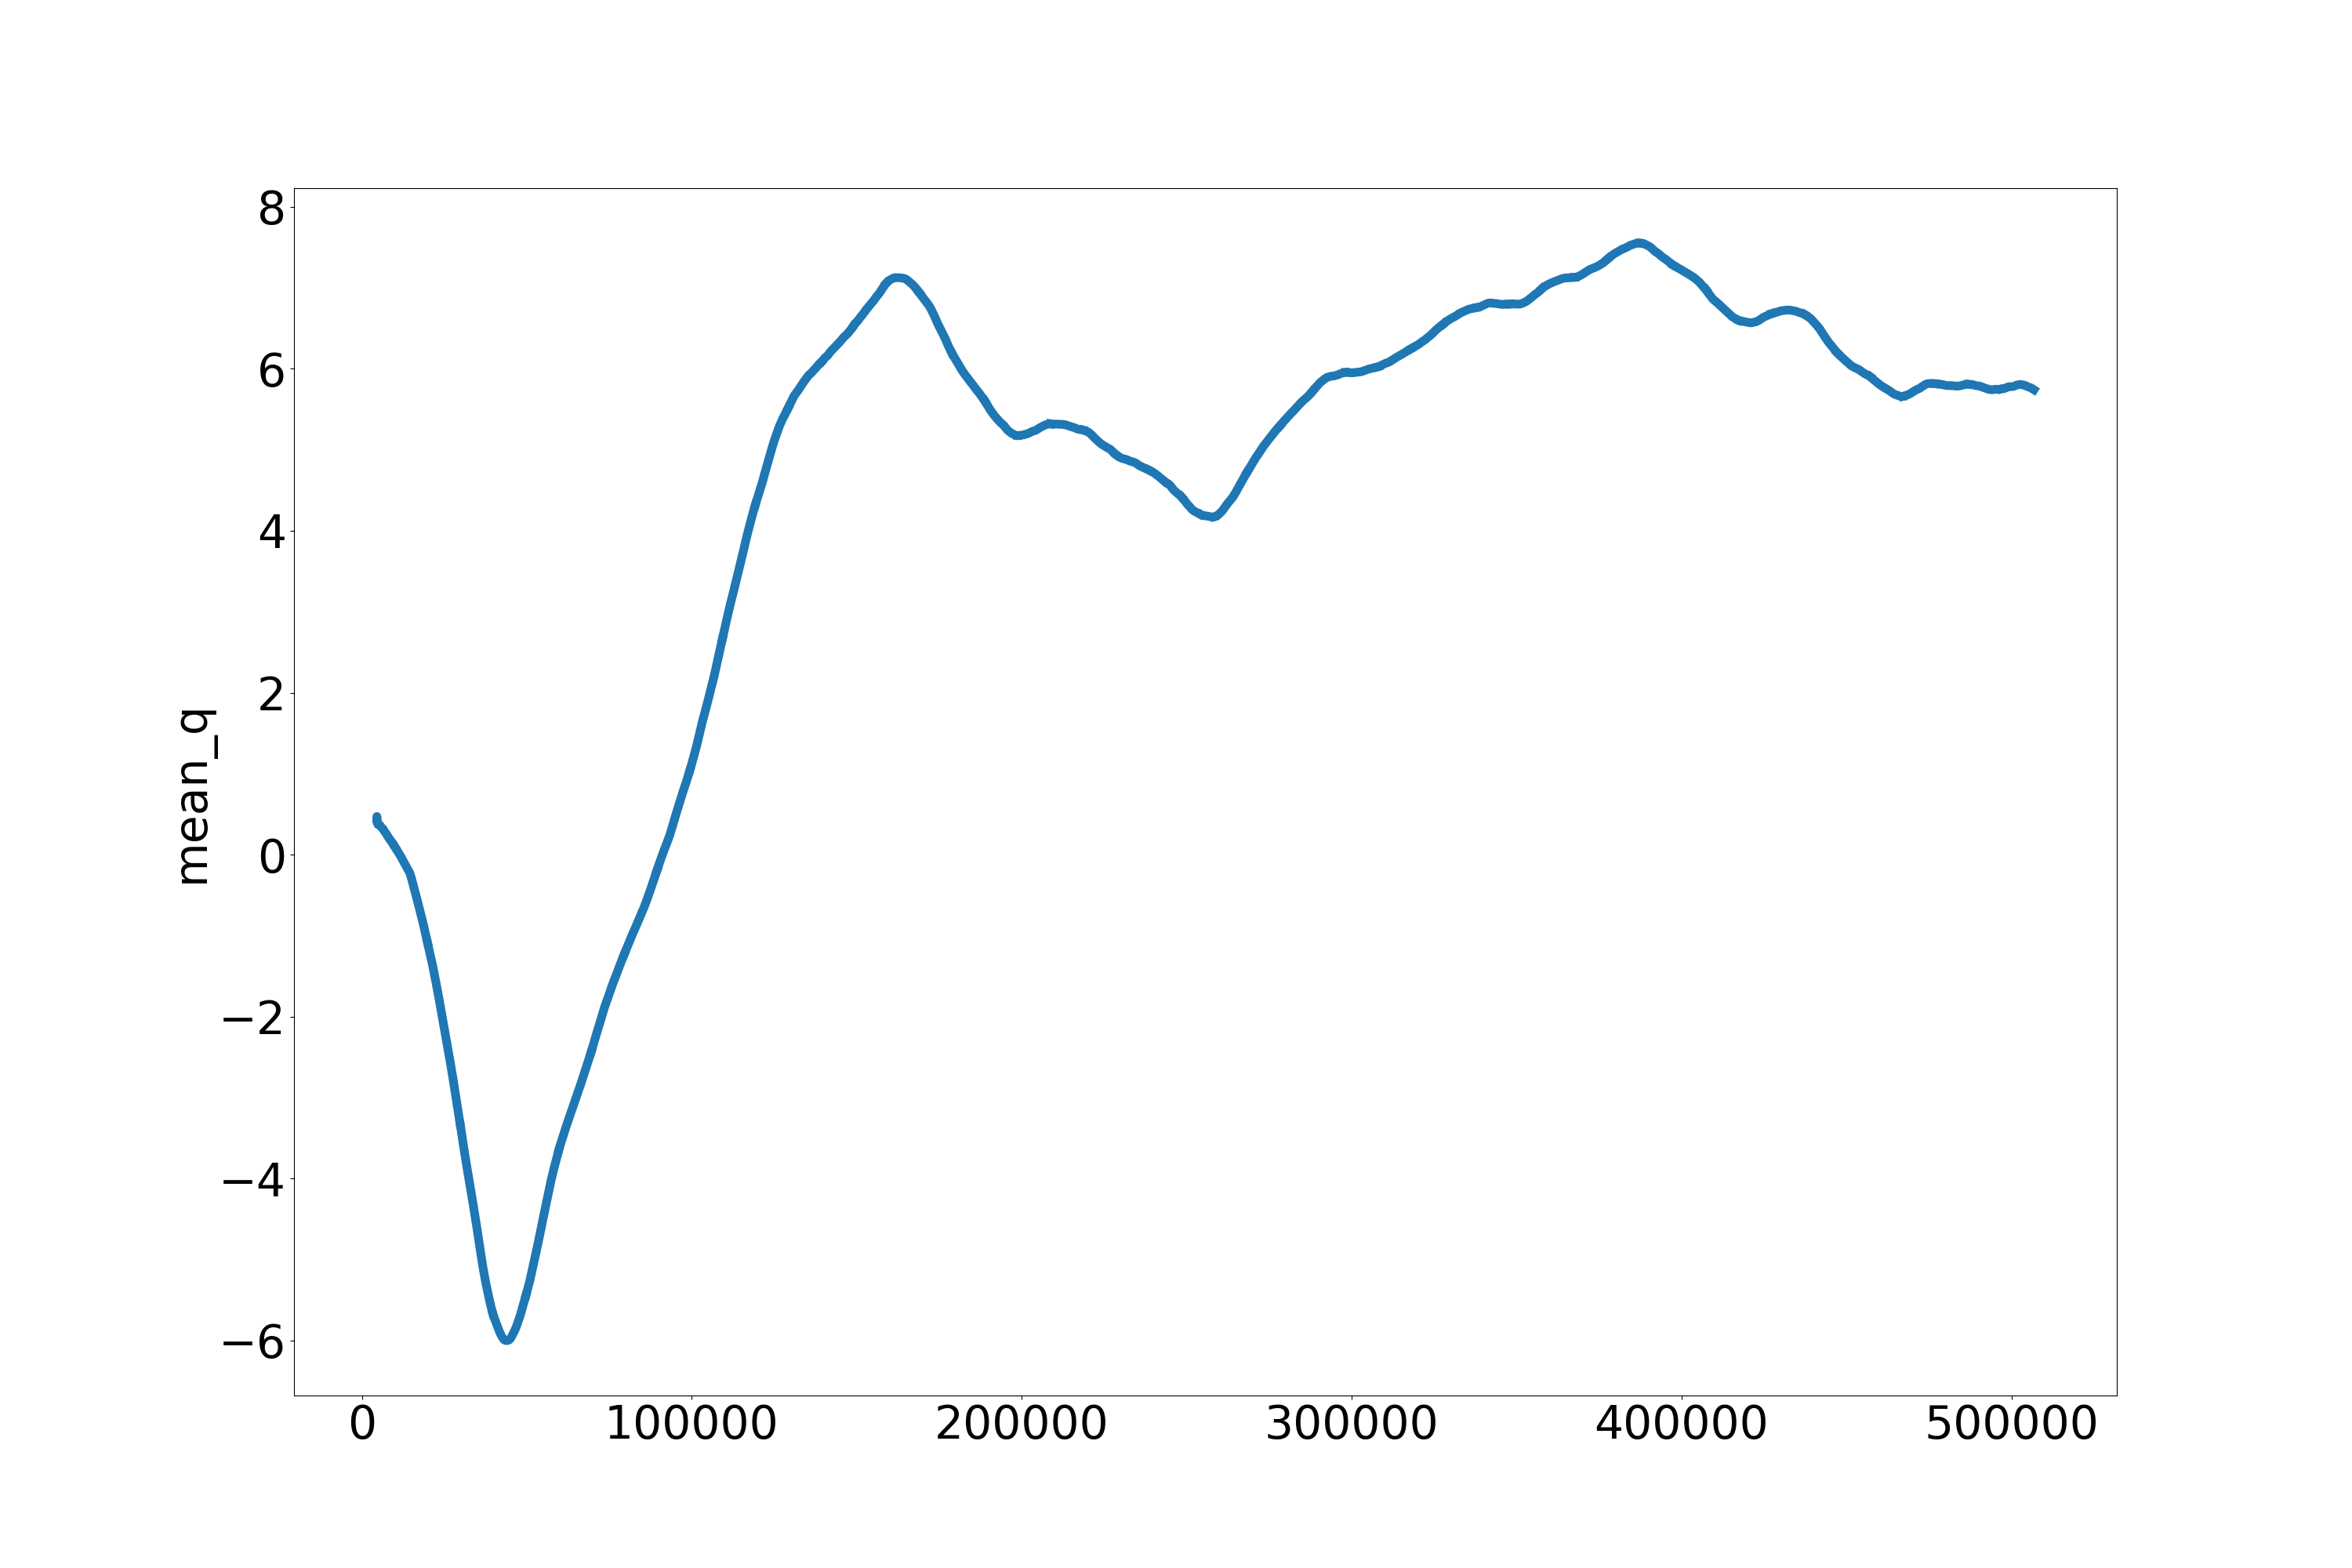
\includegraphics[width=1.1\textwidth]{Pic/Second_model/mean_q.png}  
      \caption{Trung bình giá trị Q}
      \label{fig:resut_second_model:mean_q}
    \end{subfigure}
\caption[Kết quả của mô hình thứ hai]{\textit{Kết quả của mô hình thứ hai}, có thể thấy rằng trung bình tích lũy phần thưởng chưa tăng lên vẫn còn dưới giá trị không tuy nhiên hàm mất mát chưa hội tụ và trung bình giá trị Q đạt được giá trị cao hơn so với \ref{fig:first_model:try1:mean_q}, điều này chứng tỏ mô hình vẫn có thể tốt hơn.}
\label{fig:resut_second_model}
\end{figure}
\newpage

\chapter{Kết luận} 
Khóa luận này hướng đến việc áp dụng phương pháp học tăng cường bằng thuật toán Q-learning cùng với các tùy chỉnh để chiến thắng trò chơi World's Hardest Game cho mục đích chung giải quyết bài toán tìm đường đi trong môi trường động với số bước thực hiện tối ưu. Nhóm tác giả đã đưa ra quá trình cài đặt môi trường khi đối mặt với nhiều ngôn ngữ cùng với các kinh nghiệm khi thực hiện huấn luyện trên chúng. Ngoài ra đưa ra giả thiết về trạng thái của môi trường có thể ảnh hướng đến kết quả. Các phương pháp thử nghiệm và kết quả được trình bày trong chương \ref{Chap3} và chương \ref{Chap4}. Phần thưởng là yếu tố then chốt trong việc cải thiện cách học của mô hình trong phương pháp học tăng cường. Nhiều sự cải thiện qua những thay đổi trong sự thúc đẩy và hình phạt được nhóm thực hiện trong luận văn. \\
\\
Mô hình chính mà nhóm nghiên cứu là sử dụng mạng nơ-ron để ước lượng giá trị Q sau khi thực hiện phân tích đặc trưng của môi trường. Ngoài ra, hai thành phần giúp cải thiện mô hình được sử dụng là mạng mục tiêu để tránh sự dao động quá nhiều và lịch sử kinh nghiệm giúp hàm mất mát không hội tụ nhanh trong quá trình tìm chính sách. Kết quả của mô hình không được như mong đợi khi đạt tỉ lệ thắng 55,8\% chứng tỏ rằng còn rất nhiều cải tiến có thể thực hiện với môi trường và mô hình hiện tại.    %
\clearpage
\chapter{Đề nghị nghiên cứu thêm}
Khóa luận hiện tại cần thử nghiệm trên các tùy chỉnh tốt hơn, trạng thái của môi trường có thể dùng CNN để thực hiện phân tích đặc trưng hay thiết kế hàm phần thưởng cần được chú trọng. Còn rất nhiều phương pháp học tăng cường cần được thực hiện để đạt được kết quả tốt hơn trong môi trường hiện tại. Cụ thể được đề nghị ở đây là thuật toán SARSA, đây là thuật toán học tăng cường có chính sách cũng là cách tiếp cận mới có thể thực hiện vào đề tài. \\
\\
Ngoài ra còn rất nhiều các bản đồ cần được chinh phục trong trò chơi World's Hardest Game. Cùng với các tùy chỉnh có thể tạo ra các bản đồ hay kiểm soát độ khó của chúng bằng việc thay thế mã nguồn Java của trò chơi thành Python.%
\medskip
\afterpage{\blankpage}



%Imports the bibliography file "main.bib"
\bibliographystyle{plainnat}
\bibliography{main}
\end{document}